%-----------------------------------
% Define document and include general packages
%-----------------------------------
% Tabellen- und Abbildungsverzeichnis stehen normalerweise nicht im
% Inhaltsverzeichnis. Gleiches gilt für das Abkürzungsverzeichnis (siehe unten).
% Manche Dozenten bemängeln das. Die Optionen 'listof=totoc,bibliography=totoc'
% geben das Tabellen- und Abbildungsverzeichnis im Inhaltsverzeichnis (toc=Table
% of Content) aus.
% Da es aber verschiedene Regelungen je nach Dozent geben kann, werden hier
% beide Varianten dargestellt.
\documentclass[12pt,oneside,titlepage,listof=totoc,bibliography=totoc]{scrartcl}
%\documentclass[12pt,oneside,titlepage]{scrartcl}

%-----------------------------------
% Dokumentensprache
%-----------------------------------
%\def\FOMEN{}% Auskommentieren um die Dokumentensprache auf englisch zu ändern
\newif\ifde
\newif\ifen

%-----------------------------------
% Meta informationen
%-----------------------------------
%-----------------------------------
% Meta Informationen zur Arbeit
%-----------------------------------

% Autor
\newcommand{\myAutor}{Marius Jahnke, Alexander Langel und Mike Miemczok}

% Adresse
\newcommand{\myAdresse}{Heidestra\ss e 17 \\ \> \> \> 51147 Köln}

% Titel der Arbeit
\newcommand{\myTitel}{Aufbau eines Social Media Management Systems im Kontext des DISH Plattform}

% Betreuer
\newcommand{\myBetreuer}{Prof. Dr. Rüdiger Buchkremer}

% Lehrveranstaltung
\newcommand{\myLehrveranstaltung}{Big-Data-Consultingprojekt}

% Matrikelnummer
\newcommand{\myMatrikelNr}{497615 (MJ), 487382 (AL), 491552 (MM)}

% Ort
\newcommand{\myOrt}{DLS Studium}

% Datum der Abgabe
\newcommand{\myAbgabeDatum}{\today}

% Semesterzahl
\newcommand{\mySemesterZahl}{7}

% Name der Hochschule
\newcommand{\myHochschulName}{FOM Hochschule für Oekonomie \& Management}

% Standort der Hochschule
\newcommand{\myHochschulStandort}{DLS}

% Studiengang
\newcommand{\myStudiengang}{Big Data \& Business Analytics}

% Art der Arbeit
\newcommand{\myThesisArt}{Projektarbeit}

% Zu erlangender akademische Grad
\newcommand{\myAkademischerGrad}{Master of Science (B.Sc.)}

% Firma
\newcommand{\myFirma}{Mustermann GmbH}


\ifdefined\FOMEN
%Englisch
\entrue
\usepackage[english]{babel}
\else
%Deutsch
\detrue
\usepackage[ngerman]{babel}
\fi


\newcommand{\langde}[1]{%
   \ifde\selectlanguage{ngerman}#1\fi}
\newcommand{\langen}[1]{%
   \ifen\selectlanguage{english}#1\fi}
\usepackage[utf8]{luainputenc}
\langde{\usepackage[babel,german=quotes]{csquotes}}
\langen{\usepackage[babel,english=british]{csquotes}}
\usepackage[T1]{fontenc}
\usepackage{fancyhdr}
\usepackage{fancybox}
\usepackage[a4paper, left=4cm, right=2cm, top=4cm, bottom=2cm]{geometry}
\usepackage{graphicx}
\usepackage{colortbl}
\usepackage[capposition=top]{floatrow}
\usepackage{array}
\usepackage{float}      %Positionierung von Abb. und Tabellen mit [H] erzwingen
\usepackage{footnote}
% Darstellung der Beschriftung von Tabellen und Abbildungen (Leitfaden S. 44)
% singlelinecheck=false: macht die Caption linksbündig (statt zentriert)
% labelfont auf fett: (Tabelle x.y:, Abbildung: x.y)
% font auf fett: eigentliche Bezeichnung der Abbildung oder Tabelle
% Fettschrift laut Leitfaden 2018 S. 45
\usepackage[singlelinecheck=false, labelfont=bf, font=bf]{caption}
\usepackage{caption}
\usepackage{enumitem}
\usepackage{amssymb}
\usepackage{mathptmx}
%\usepackage{minted} %Kann für schöneres Syntax Highlighting genutzt werden. ACHTUNG: Python muss installiert sein.
\usepackage[scaled=0.9]{helvet} % Behebt, zusammen mit Package courier, pixelige Überschriften. Ist, zusammen mit mathptx, dem times-Package vorzuziehen. Details: https://latex-kurs.de/fragen/schriftarten/Times_New_Roman.html
\usepackage{courier}
\usepackage{amsmath}
\usepackage[table]{xcolor}
\usepackage{marvosym}			% Verwendung von Symbolen, z.B. perfektes Eurozeichen

\renewcommand\familydefault{\sfdefault}
\usepackage{ragged2e}

% Mehrere Fussnoten nacheinander mit Komma separiert
\usepackage[hang,multiple]{footmisc}
\setlength{\footnotemargin}{1em}

% todo Aufgaben als Kommentare verfassen für verschiedene Editoren
\usepackage{todonotes}

% Verhindert, dass nur eine Zeile auf der nächsten Seite steht
\setlength{\marginparwidth}{2cm}
\usepackage[all]{nowidow}

%-----------------------------------
% Farbdefinitionen
%-----------------------------------
\definecolor{darkblack}{rgb}{0,0,0}
\definecolor{dunkelgrau}{rgb}{0.8,0.8,0.8}
\definecolor{hellgrau}{rgb}{0.0,0.7,0.99}
\definecolor{mauve}{rgb}{0.58,0,0.82}
\definecolor{dkgreen}{rgb}{0,0.6,0}

%-----------------------------------
% Pakete für Tabellen
%-----------------------------------
\usepackage{epstopdf}
\usepackage{nicefrac} % Brüche
\usepackage{multirow}
\usepackage{rotating} % vertikal schreiben
\usepackage{mdwlist}
\usepackage{tabularx}% für Breitenangabe

%-----------------------------------
% sauber formatierter Quelltext
%-----------------------------------
\usepackage{listings}
% JavaScript als Sprache definieren:
\lstdefinelanguage{JavaScript}{
	keywords={break, super, case, extends, switch, catch, finally, for, const, function, try, continue, if, typeof, debugger, var, default, in, void, delete, instanceof, while, do, new, with, else, return, yield, enum, let, await},
	keywordstyle=\color{blue}\bfseries,
	ndkeywords={class, export, boolean, throw, implements, import, this, interface, package, private, protected, public, static},
	ndkeywordstyle=\color{darkgray}\bfseries,
	identifierstyle=\color{black},
	sensitive=false,
	comment=[l]{//},
	morecomment=[s]{/*}{*/},
	commentstyle=\color{purple}\ttfamily,
	stringstyle=\color{red}\ttfamily,
	morestring=[b]',
	morestring=[b]"
}

\lstset{
	%language=JavaScript,
	numbers=left,
	numberstyle=\tiny,
	numbersep=5pt,
	breaklines=true,
	showstringspaces=false,
	frame=l ,
	xleftmargin=5pt,
	xrightmargin=5pt,
	basicstyle=\ttfamily\scriptsize,
	stepnumber=1,
	keywordstyle=\color{blue},          % keyword style
  	commentstyle=\color{dkgreen},       % comment style
  	stringstyle=\color{mauve}         % string literal style
}

%-----------------------------------
%Literaturverzeichnis Einstellungen
%-----------------------------------

% Biblatex

\usepackage{url}
\urlstyle{same}

%%%% Neuer Leitfaden (2018)
\usepackage[
backend=biber,
style=ext-authoryear-ibid, % Auskommentieren und nächste Zeile einkommentieren, falls "Ebd." (ebenda) nicht für sich-wiederholende Fussnoten genutzt werden soll.
%style=ext-authoryear,
maxcitenames=3,	% mindestens 3 Namen ausgeben bevor et. al. kommt
maxbibnames=999,
mergedate=false,
date=iso,
seconds=true, %werden nicht verwendet, so werden aber Warnungen unterdrückt.
urldate=iso,
innamebeforetitle,
dashed=false,
autocite=footnote,
doi=false,
useprefix=true, % 'von' im Namen beachten (beim Anzeigen)
mincrossrefs = 1
]{biblatex}%iso dateformat für YYYY-MM-DD

%weitere Anpassungen für BibLaTex
\usepackage{xpatch}

\setlength\bibhang{1cm}

%%% Weitere Optionen
%\boolitem[false]{citexref} %Wenn incollection, inbook, inproceedings genutzt wird nicht den zugehörigen parent auch in Literaturverzeichnis aufnehmen

%Aufräumen die Felder werden laut Leitfaden nicht benötigt.
\AtEveryBibitem{%
\ifentrytype{book}{
    \clearfield{issn}%
    \clearfield{doi}%
    \clearfield{isbn}%
    \clearfield{url}
    \clearfield{eprint}
}{}
\ifentrytype{collection}{
  \clearfield{issn}%
  \clearfield{doi}%
  \clearfield{isbn}%
  \clearfield{url}
  \clearfield{eprint}
}{}
\ifentrytype{incollection}{
  \clearfield{issn}%
  \clearfield{doi}%
  \clearfield{isbn}%
  \clearfield{url}
  \clearfield{eprint}
}{}
\ifentrytype{article}{
  \clearfield{issn}%
  \clearfield{doi}%
  \clearfield{isbn}%
  \clearfield{url}
  \clearfield{eprint}
}{}
\ifentrytype{inproceedings}{
  \clearfield{issn}%
  \clearfield{doi}%
  \clearfield{isbn}%
  \clearfield{url}
  \clearfield{eprint}
}{}
}

\renewcommand*{\finentrypunct}{}%Kein Punkt am ende des Literaturverzeichnisses

\renewcommand*{\newunitpunct}{\addcomma\space}
\DeclareDelimFormat[bib,biblist]{nametitledelim}{\addcolon\space}
\DeclareDelimFormat{titleyeardelim}{\newunitpunct}
%Namen kursiv schreiben
\renewcommand*{\mkbibnamefamily}{\mkbibemph}
\renewcommand*{\mkbibnamegiven}{\mkbibemph}
\renewcommand*{\mkbibnamesuffix}{\mkbibemph}
\renewcommand*{\mkbibnameprefix}{\mkbibemph}

% Die Trennung mehrerer Autorennamen erfolgt durch Kommata.
% siehe Beispiele im Leitfaden S. 16
% Die folgende Zeile würde mit Semikolon trennen
%\DeclareDelimFormat{multinamedelim}{\addsemicolon\addspace}

%Delimiter für mehrere und letzten Namen gleich setzen
\DeclareDelimAlias{finalnamedelim}{multinamedelim}

\DeclareNameAlias{default}{family-given}
\DeclareNameAlias{sortname}{default}  %Nach Namen sortieren


\DeclareFieldFormat{editortype}{\mkbibparens{#1}}
\DeclareDelimFormat{editortypedelim}{\addspace}
\DeclareFieldFormat{translatortype}{\mkbibparens{#1}}
\DeclareDelimFormat{translatortypedelim}{\addspace}
\DeclareDelimFormat[bib,biblist]{innametitledelim}{\addcomma\space}

\DeclareFieldFormat*{citetitle}{#1}
\DeclareFieldFormat*{title}{#1}
\DeclareFieldFormat*{booktitle}{#1}
\DeclareFieldFormat*{journaltitle}{#1}

\xpatchbibdriver{online}
  {\usebibmacro{organization+location+date}\newunit\newblock}
  {}
  {}{}

\DeclareFieldFormat[online]{date}{\mkbibparens{#1}}
\DeclareFieldFormat{urltime}{\addspace #1\addspace \langde{Uhr}\langen{MEZ}}
\DeclareFieldFormat{urldate}{%urltime zu urldate hinzufügen
  [\langde{Zugriff}\langen{Access}\addcolon\addspace
  #1\printfield{urltime}]
}
\DeclareFieldFormat[online]{url}{<\url{#1}>}
\renewbibmacro*{url+urldate}{%
  \usebibmacro{url}%
  \ifentrytype{online}
    {\setunit*{\addspace}%
     \iffieldundef{year}
       {\printtext[date]{\langde{keine Datumsangabe}\langen{no Date} }}
       {\usebibmacro{date}}}%
    {}%
  \setunit*{\addspace}%
  \usebibmacro{urldate}
  }

%Verhindern, dass bei mehreren Quellen des gleichen Autors im gleichen Jahr
%Buchstaben nach der Jahreszahl angezeigt werden wenn sich das Keyword in usera unterscheidet.
\DeclareExtradate{
  \scope{
    \field{labelyear}
    \field{year}
    }
    \scope{
      \field{usera}
     }
}

%% Anzeige des Jahres nach dem Stichwort (usera) im Literaturverzeichnis
%% Wenn das Jahr bei Online-Quellen nicht explizit angegeben wurde, wird nach
%% dem Stichwort 'o. J.' ausgegeben. Nach der URL steht dann 'keine
%% Datumsangabe'. Ist das Jahr definiert, wird es an beiden Stellen ausgegeben.
%% Das Zugriffsdatum (urldate) spielt hier keine Rolle.
%% Für Nicht-Online-Quellen wird nichts geändert.
\renewbibmacro*{date+extradate}{%
  \printtext[parens]{%
    \printfield{usera}%
    \setunit{\printdelim{titleyeardelim}}%
    \ifentrytype{online}
       {\setunit*{\addspace\addcomma\addspace}%
         \iffieldundef{year}
           {\bibstring{nodate}}
       {\printlabeldateextra}}%
       {\printlabeldateextra}}}

%% Anzeige des Jahres nach dem Stichwort (usera) in der Fussnote
%% das Stichwort hat der Aufrufer hier schon ausgegeben.
%% siehe auch Kommentar zu: \renewbibmacro*{date+extradate}
\renewbibmacro*{cite:labeldate+extradate}{%
    \ifentrytype{online}
       {\setunit*{\addspace\addcomma\addspace}%
         \iffieldundef{year}
           {\bibstring{nodate}}
       {\printlabeldateextra}}%
       {\printlabeldateextra}}


\DefineBibliographyStrings{german}{
  nodate    = {{}o.\adddot\addspace J\adddot},
  andothers = {et\addabbrvspace al\adddot}
}
\DefineBibliographyStrings{english}{
  nodate    = {{}n.\adddot\addspace d\adddot},
  andothers = {et\addabbrvspace al\adddot}
}
\DeclareSourcemap{
  \maps[datatype=bibtex]{
    \map{
      \step[notfield=translator, final]
      \step[notfield=editor, final]
      \step[fieldset=author, fieldvalue={{{\langde{o\noexpand\adddot\addspace V\noexpand\adddot}\langen{Anon}}}}]
    }
    \map{
      \pernottype{online}
      \step[fieldset=location, fieldvalue={\langde{o\noexpand\adddot\addspace O\noexpand\adddot}\langen{s\noexpand\adddot I\noexpand\adddot}}]
    }
  }
}

\renewbibmacro*{cite}{%
  \iffieldundef{shorthand}
    {\ifthenelse{\ifnameundef{labelname}\OR\iffieldundef{labelyear}}
       {\usebibmacro{cite:label}%
        \setunit{\printdelim{nonametitledelim}}}
       {\printnames{labelname}%
        \setunit{\printdelim{nametitledelim}}}%
     \printfield{usera}%
     \setunit{\printdelim{titleyeardelim}}%
     \usebibmacro{cite:labeldate+extradate}}
    {\usebibmacro{cite:shorthand}}}

    \renewcommand*{\jourvoldelim}{\addcomma\addspace}% Trennung zwischen journalname und Volume. Sonst Space; Laut Leitfaden richtig
    %Aufgrund der Änderung bzgl des Issues 169 in der thesis_main.tex musste ich die Zeile auskommentieren. Konnte aber das Verhalten, dass die Fußnoten grün sind, im nachhinein nicht feststellen.
    %\hypersetup{hidelinks} %sonst sind Fußnoten grün. Dadurch werden Links allerdings nicht mehr farbig dargestellt

\renewbibmacro*{journal+issuetitle}{%
  \usebibmacro{journal}%
  \setunit*{\jourvoldelim}%
  \iffieldundef{series}
    {}
    {\setunit*{\jourserdelim}%
     \printfield{series}%
     \setunit{\servoldelim}}%
  \iffieldundef{volume}
    {}
    {\printfield{volume}}
  \iffieldundef{labelyear}
  {}
  {
  (\thefield{year}) %Ansonsten wird wenn kein Volume angegeben ist ein Komma vorangestellt
  }
  \setunit*{\addcomma\addspace Nr\adddot\addspace}
  \printfield{number}
  \iffieldundef{eid}
  {}
  {\printfield{eid}}
}

% Postnote ist der Text in der zweiten eckigen Klammer bei einem Zitat
% wenn es keinen solchen Eintrag gibt, dann auch nicht ausgeben, z.B. 'o. S.'
% Wenn man das will, kann man das 'o. S.' ja explizit angeben. Andernfalls steht
% sonst auch bei Webseiten 'o. S.' da, was laut Leitfaden nicht ok ist.
\renewbibmacro*{postnote}{%
  \setunit{\postnotedelim}%
  \iffieldundef{postnote}
    {} %{\printtext{\langde{o.S\adddot}\langen{no page number}}}
    {\printfield{postnote}}}

% Abstand bei Änderung Anfangsbuchstabe ca. 1.5 Zeilen
\setlength{\bibinitsep}{0.75cm}

% nur in den Zitaten/Fussnoten den Vornamen abkürzen (nicht im
% Literaturverzeichnis)

\DeclareDelimFormat{nonameyeardelim}{\addcomma\space}
\DeclareDelimFormat{nameyeardelim}{\addcomma\space}

\renewbibmacro*{cite}{%
  \iffieldundef{shorthand}
    {\ifthenelse{\ifciteibid\AND\NOT\iffirstonpage}
       {\usebibmacro{cite:ibid}}
    {\printtext[bibhyperref]{\ifthenelse{\ifnameundef{labelname}\OR\iffieldundef{labelyear}}
       {\usebibmacro{cite:label}%
        \setunit{\printdelim{nonameyeardelim}}}
      {\toggletrue{abx@bool@giveninits}%
        \printnames[family-given]{labelname}%
        \setunit{\printdelim{nameyeardelim}}}%
      \printfield{usera}%
      \setunit{\printdelim{titleyeardelim}}%
     \usebibmacro{cite:labeldate+extradate}}}}
   {\usebibmacro{cite:shorthand}}}

\renewcommand{\footcite}[2][]{\footnote{Vgl. \cite[#1]{#2}.}}

%%%%% Alter Leitfaden. Ggf. Einkommentieren und Bereich hierüber auskommentieren
%\usepackage[
%backend=biber,
%style=numeric,
%citestyle=authoryear,
%url=false,
%isbn=false,
%notetype=footonly,
%hyperref=false,
%sortlocale=de]{biblatex}

%weitere Anpassungen für BibLaTex
%% Opptionen für Biblatex
\ExecuteBibliographyOptions{%
giveninits=false,
isbn=true,
url=true,
doi=false,
eprint=false,
maxbibnames=7, % Alle Autoren (kein et al.)
maxcitenames=2, % et al. ab dem 3. Autor
backref=false, % Rückverweise auf Zitatseiten
bibencoding=utf8, % wenn .bib in utf8, sonst ascii
bibwarn=true, % Warnung bei fehlerhafter bib-Datei
}%

% et al. an Stelle von u.a.
\DefineBibliographyStrings{ngerman}{
   andothers = {{et\,al\adddot}},
}

% Klammern um das Jahr in der Fußnote
\renewbibmacro*{cite:labelyear+extrayear}{%
  \iffieldundef{labelyear}
    {}
    {\printtext[bibhyperref]{%
       \mkbibparens{%
         \printfield{labelyear}%
         \printfield{extrayear}}}}}

\renewbibmacro*{cite:title}{%
  \printtext[bibhyperref]{%
    \printfield[citetitle]{labeltitle}%
    \setunit{\addcomma\space}%
    \printdate}}

\DeclareNameFormat{last-first}{%
  \iffirstinits
    {\usebibmacro{name:family-given}
        {\namepartfamily}
        {\namepartgiveni}
        {\namepartprefix}
        {\namepartsuffix}
    }
    {\usebibmacro{name:family-given}
        {\namepartfamily}
        {\namepartgiven}
        {\namepartprefix}
        {\namepartsuffix}
    }%
  \usebibmacro{name:andothers}}

% Alternative Notation der Fußnoten
% Zeigt sowohl den Nachnamen als auch den Vornamen an
% Beispiel: \fullfootcite[Vgl. ][Seite 5]{Tanenbaum.2003}
\DeclareCiteCommand{\fullfootcite}[\mkbibfootnote]
  {\usebibmacro{prenote}}
  {\usebibmacro{citeindex}%
    \printnames[sortname][1-1]{author}%
    \addspace (\printfield{year})}
  {\addsemicolon\space}
  {\usebibmacro{postnote}}

%Autoren (Nachname, Vorname)
\DeclareNameAlias{default}{family-given}

%Reihenfolge von publisher, year, address verändern
% Achtung, bisher nur für den Typ @book definiert

%% Definiert @Book Eintrag
\DeclareBibliographyDriver{book}{%
  \printnames{author}%
  \newunit\addcolon\space
  \printfield{title}%
  \setunit*{,\space}%
  \printfield{edition}%
  \setunit*{\addcomma\space}%
  \printlist{publisher}%
  \newunit\newblockpunct
  \printlist{location}%
  \setunit*{\space}%
  \printfield{year}%
  \setunit*{,\space}%
  \printfield{isbn}%
  \finentry}

%% Definiert @Online Eintrag
\DeclareBibliographyDriver{online}{%
  \printnames{author}%
  \newunit\newblockpunct
  \printfield{title}%
  \setunit*{,\space}%
  %\newunit\newblock
  \printfield{url}%
  \setunit*{,\space Erscheinungsjahr:\space}%
  \printfield{year}%
  \setunit*{,\space Aufruf am:\space}%
  \printfield{note}%
  \finentry}

%% Definiert @Article Eintrag
\DeclareBibliographyDriver{article}{%
  \printnames{author}%
  \newunit\newblockpunct
  \printfield{title}%
  \setunit*{.\space In:\space}%
  %\newunit\newblock
  \usebibmacro{journal}%
  \setunit*{\space (}%
  \printfield{year}\newunit{)}%
  \finentry}

%% Definiert @InProceedings Eintrag
\DeclareBibliographyDriver{inproceedings}{%
	\printnames{author}%
	\setunit*{,\space (}%
	\printfield{year}\newunit{)}%
	\newunit\newblockpunct
	\printfield{title}%
	\setunit*{\space}%
	\usebibmacro{booktitle}%
	\setunit*{,\space}%
	\printfield{isbn}%
	\setunit*{,\space}%
	\printfield{doi}%
	\finentry}

%Doppelpunkt nach dem letzten Autor
\renewcommand*{\labelnamepunct}{\addcolon\addspace }

%Komma an Stelle des Punktes
\renewcommand*{\newunitpunct}{\addcomma\space}

%Autoren durch Semikolon trennen
\newcommand*{\bibmultinamedelim}{\addsemicolon\space}%
\newcommand*{\bibfinalnamedelim}{\addsemicolon\space}%
\AtBeginBibliography{%
  \let\multinamedelim\bibmultinamedelim
  \let\finalnamedelim\bibfinalnamedelim
}

%Titel nicht kursiv anzeigen
\DeclareFieldFormat{title}{#1\isdot}


%%%% Ende Alter Leitfaden

%Bib-Datei einbinden
\addbibresource{literatur/literatur.bib}

% Zeilenabstand im Literaturverzeichnis ist Einzeilig
% siehe Leitfaden S. 14
\AtBeginBibliography{\singlespacing}

%-----------------------------------
% Silbentrennung
%-----------------------------------
\usepackage{hyphsubst}
\HyphSubstIfExists{ngerman-x-latest}{%
\HyphSubstLet{ngerman}{ngerman-x-latest}}{}

%-----------------------------------
% Pfad fuer Abbildungen
%-----------------------------------
\graphicspath{{./}{./abbildungen/}}

%-----------------------------------
% Weitere Ebene einfügen
%-----------------------------------
\usepackage{titletoc}

\makeatletter

% Setze die Tiefe des Inhaltsverzeichnis auf 4 Ebenen
% Damit erscheinen \paragraph-Sektionen auch im Inhaltsverzeichnis
\setcounter{secnumdepth}{4}
\setcounter{tocdepth}{4}

% Fuege Abstand nach unten wie in einer normalen \section hinzu
% Andernfalls haette \paragraph keinen Zeilenumbruch
% Der Zeilenumbruch koennte mit einer leeren \mbox{} ersetzt werden
% Jedoch klebt dann der Text relativ nah an der Ueberschrift
\renewcommand{\paragraph}{%
  \@startsection{paragraph}{4}%
  {\z@}{3.25ex \@plus 1ex \@minus .2ex}{1.5ex plus 0.2ex}%
  {\normalfont\normalsize\bfseries\sffamily}%
}

\makeatother


%-----------------------------------
% Paket für die Nutzung von Anhängen
%-----------------------------------
\usepackage{appendix}

%-----------------------------------
% Zeilenabstand 1,5-zeilig
%-----------------------------------
\usepackage{setspace}
\onehalfspacing

%-----------------------------------
% Absätze durch eine neue Zeile
%-----------------------------------
\setlength{\parindent}{0mm}
\setlength{\parskip}{0.8em plus 0.5em minus 0.3em}

\sloppy					%Abstände variieren
\pagestyle{headings}

%----------------------------------
% Präfix in das Abbildungs- und Tabellenverzeichnis aufnehmen, statt nur der Nummerierung (siehe Issue #206).
%----------------------------------
\KOMAoption{listof}{entryprefix} % Siehe KOMA-Script Doku v3.28 S.153
\BeforeStartingTOC[lof]{\renewcommand*\autodot{:}} % Für den Doppelpunkt hinter Präfix im Abbildungsverzeichnis
\BeforeStartingTOC[lot]{\renewcommand*\autodot{:}} % Für den Doppelpunkt hinter Präfix im Tabellenverzeichnis

%-----------------------------------
% Abkürzungsverzeichnis
%-----------------------------------
\usepackage[printonlyused]{acronym}

%-----------------------------------
% Symbolverzeichnis
%-----------------------------------
% Quelle: https://www.namsu.de/Extra/pakete/Listofsymbols.pdf
\usepackage[final]{listofsymbols}

%-----------------------------------
% Glossar
%-----------------------------------
\usepackage{glossaries}
\glstoctrue %Auskommentieren, damit das Glossar nicht im Inhaltsverzeichnis angezeigt wird.
\makenoidxglossaries
\newglossaryentry{glossar}{name={Glossar},description={In einem Glossar werden Fachbegriffe und Fremdwörter mit ihren Erklärungen gesammelt.}}
\newglossaryentry{glossaries}{name={Glossaries},description={Glossaries ist ein Paket was einen im Rahmen von LaTeX bei der Erstellung eines Glossar unterstützt.}}


%-----------------------------------
% PDF Meta Daten setzen
%-----------------------------------
\usepackage[hyperfootnotes=false]{hyperref} %hyperfootnotes=false deaktiviert die Verlinkung der Fußnote. Ansonsten inkompaibel zum Paket "footmisc"
% Behebt die falsche Darstellung der Lesezeichen in PDF-Dateien, welche eine Übersetzung besitzen
% siehe Issue 149
\makeatletter
\pdfstringdefDisableCommands{\let\selectlanguage\@gobble}
\makeatother

\hypersetup{
    pdfinfo={
        Title={\myTitel},
        Subject={\myStudiengang},
        Author={\myAutor},
        Build=1.1
    }
}

%-----------------------------------
% PlantUML
%-----------------------------------
%\usepackage{plantuml}

%-----------------------------------
% Umlaute in Code korrekt darstellen
% siehe auch: https://en.wikibooks.org/wiki/LaTeX/Source_Code_Listings
%-----------------------------------
\lstset{literate=
	{á}{{\'a}}1 {é}{{\'e}}1 {í}{{\'i}}1 {ó}{{\'o}}1 {ú}{{\'u}}1
	{Á}{{\'A}}1 {É}{{\'E}}1 {Í}{{\'I}}1 {Ó}{{\'O}}1 {Ú}{{\'U}}1
	{à}{{\`a}}1 {è}{{\`e}}1 {ì}{{\`i}}1 {ò}{{\`o}}1 {ù}{{\`u}}1
	{À}{{\`A}}1 {È}{{\'E}}1 {Ì}{{\`I}}1 {Ò}{{\`O}}1 {Ù}{{\`U}}1
	{ä}{{\"a}}1 {ë}{{\"e}}1 {ï}{{\"i}}1 {ö}{{\"o}}1 {ü}{{\"u}}1
	{Ä}{{\"A}}1 {Ë}{{\"E}}1 {Ï}{{\"I}}1 {Ö}{{\"O}}1 {Ü}{{\"U}}1
	{â}{{\^a}}1 {ê}{{\^e}}1 {î}{{\^i}}1 {ô}{{\^o}}1 {û}{{\^u}}1
	{Â}{{\^A}}1 {Ê}{{\^E}}1 {Î}{{\^I}}1 {Ô}{{\^O}}1 {Û}{{\^U}}1
	{œ}{{\oe}}1 {Œ}{{\OE}}1 {æ}{{\ae}}1 {Æ}{{\AE}}1 {ß}{{\ss}}1
	{ű}{{\H{u}}}1 {Ű}{{\H{U}}}1 {ő}{{\H{o}}}1 {Ő}{{\H{O}}}1
	{ç}{{\c c}}1 {Ç}{{\c C}}1 {ø}{{\o}}1 {å}{{\r a}}1 {Å}{{\r A}}1
	{€}{{\EUR}}1 {£}{{\pounds}}1 {„}{{\glqq{}}}1
}

%-----------------------------------
% Kopfbereich / Header definieren
%-----------------------------------
\pagestyle{fancy}
\fancyhf{}
% Seitenzahl oben, mittig, mit Strichen beidseits
% \fancyhead[C]{-\ \thepage\ -}

% Seitenzahl oben, mittig, entsprechend Leitfaden ohne Striche beidseits
\fancyhead[C]{\thepage}
%\fancyhead[L]{\leftmark}							% kein Footer vorhanden
% Waagerechte Linie unterhalb des Kopfbereiches anzeigen. Laut Leitfaden ist
% diese Linie nicht erforderlich. Ihre Breite kann daher auf 0pt gesetzt werden.
\renewcommand{\headrulewidth}{0.4pt}
%\renewcommand{\headrulewidth}{0pt}

%-----------------------------------
% Damit die hochgestellten Zahlen auch auf die Fußnote verlinkt sind (siehe Issue 169)
%-----------------------------------
\hypersetup{colorlinks=true, breaklinks=true, linkcolor=darkblack, citecolor=darkblack, menucolor=darkblack, urlcolor=darkblack, linktoc=all, bookmarksnumbered=false, pdfpagemode=UseOutlines, pdftoolbar=true}
\urlstyle{same}%gleiche Schriftart für den Link wie für den Text

%-----------------------------------
% Start the document here:
%-----------------------------------
\begin{document}

\pagenumbering{Roman}								% Seitennumerierung auf römisch umstellen
\newcolumntype{C}{>{\centering\arraybackslash}X}	% Neuer Tabellen-Spalten-Typ:
%Zentriert und umbrechbar

%-----------------------------------
% Textcommands
%-----------------------------------
%----------------------------------
%  TextCommands
%----------------------------------
%
%
%
%
%----------------------------------
%  common textCommands
%----------------------------------
% Information: OL bedeutet ohne Leerzeichen. Damit man dieses Command z. B. vor einem Komma oder vor einem anderen Zeichen verwenden kann. Dies ist ein Best-Practis von mir und hat sich sehr bewehrt.
% Allgemein hat es sich bewert alle Wörter die man häufig schreibt und wahrscheinlich falsch oder unterscheidlich schreibt, als Textcommand zu hinterlegen.
% 
%
%
\renewcommand{\symheadingname}{\langde{Symbolverzeichnis}\langen{List of Symbols}}
\newcommand{\abbreHeadingName}{\langde{Abkürzungsverzeichnis}\langen{List of Abbreviations}}
\newcommand{\headingNameInternetSources}{\langde{Internetquellen}\langen{Internet sources}}
\newcommand{\AppendixName}{\langde{Anhang}\langen{Appendix}}
\newcommand{\vglf}{\langde{Vgl.}\langen{compare}}
\newcommand{\pagef}{\langde{S. }\langen{p. }}
\newcommand{\os}{\mbox{o. S}}
\newcommand{\ojol}{\mbox{o. J.}}
\newcommand{\oj}{\ojol\ }
\newcommand{\og}{\mbox{o. g.}\ }
\newcommand{\ua}{\mbox{u. a.}\ }
\newcommand{\dah}{\mbox{d. h.}\ }
\newcommand{\zbol}{\mbox{z. B.}}
\newcommand{\zb}{\zbol\ }
\newcommand{\uamol}{unter anderem}
\newcommand{\uam}{\uamol\ }
\newcommand{\uanol}{unter anderen}%mit Leerzeichen
\newcommand{\uan}{\uanol\ }%mit Leerzeichen
\newcommand{\abbol}{Ab"-bil"-dung}
\newcommand{\abb}{\abbol\ }
\newcommand{\tabol}{Tabelle}
\newcommand{\tab}{\tabol\ }
\newcommand{\ggfol}{ggf.}
\newcommand{\ggf}{\ggfol\ }
\newcommand{\unodol}{und/oder}
\newcommand{\unod}{\unodol\ }

%----------------------------------
% project individual textCommands
%----------------------------------
\newcommand{\lehol}{Lebensmitteleinzelhandel}%Beispiel eines langen Wortes
\newcommand{\leh}{\lehol\ }


%-----------------------------------
% Titlepage
%-----------------------------------
\begin{titlepage}
	\newgeometry{left=2cm, right=2cm, top=2cm, bottom=2cm}
	\begin{center}
    
\includegraphics[width=2.3cm]{abbildungen/fomLogo} \\
    \vspace{.5cm}
		\begin{Large}\textbf{\myHochschulName}\end{Large}\\
    \vspace{.5cm}
		\begin{Large}\langde{Hochschulzentrum}\langen{university location} \myHochschulStandort\end{Large}\\
		\vspace{2cm}
    \begin{Large}\textbf{\myThesisArt}\end{Large}\\
    \vspace{.5cm}
		% \langde{Berufsbegleitender Studiengang}
		% \langen{part-time degree program}\\
		% \mySemesterZahl. Semester\\
    \langde{im Studiengang}\langen{in the study course} \myStudiengang
		\vspace{1.7cm}

		% \langde{zur Erlangung des Grades eines}\langen{to obtain the degree of}\\
    % \vspace{0.5cm}
		% \begin{Large}{\myAkademischerGrad}\end{Large}\\
		% Oder für Hausarbeiten:
		\langde{im Rahmen der Lehrveranstaltung}\\
		\textbf{\myLehrveranstaltung}\\
		\vspace{1.8cm}
		\langde{über das Thema}
		\langen{on the subject}\\
    \vspace{0.5cm}
		\large{\textbf{\myTitel}}\\
		\vspace{2cm}
    \langde{von}\langen{by}\\
    \vspace{0.5cm}
    \begin{Large}{\myAutor}\end{Large}\\
	\end{center}
	\normalsize
	\vfill
    \begin{tabular}{ l l }
        \langde{Betreuer} % für Hausarbeiten
        %\langde{Erstgutachter} % für Bachelor- / Master-Thesis
        \langen{Advisor}: & \myBetreuer\\
        \langde{Matrikelnummer}
        \langen{Matriculation Number}: & \myMatrikelNr\\
        \langde{Abgabedatum}
        \langen{Submission}: & \myAbgabeDatum
    \\
    \end{tabular}
\end{titlepage}


%-----------------------------------
% Vorwort (optional; bei Verwendung beide Zeilen entkommentieren und unter Inhaltsverzeichnis setcounter entsprechend anpassen)
%-----------------------------------
%\section*{Vorwort}
Bei Bedarf erscheint vor dem Inhaltsverzeichnis ein Vorwort. Es erhält keine Kapitelnummer und wird nicht im Inhaltsverzeichnis aufgeführt (Auszug aus dem Leitfaden zur Gestaltung wissenschaftlicher Arbeiten / Dekanat ING \& IT Management, Februar 2022).

Lorem ipsum dolor sit amet, consetetur sadipscing elitr, sed diam nonumy eirmod tempor invidunt ut labore et dolore magna aliquyam erat, sed diam voluptua. At vero eos et accusam et justo duo dolores et ea rebum. Stet clita kasd gubergren, no sea takimata sanctus est Lorem ipsum dolor sit amet. Lorem ipsum dolor sit amet, consetetur sadipscing elitr, sed diam nonumy eirmod tempor invidunt ut labore et dolore magna aliquyam erat, sed diam voluptua. At vero eos et accusam et justo duo dolores et ea rebum. Stet clita kasd gubergren, no sea takimata sanctus est Lorem ipsum dolor sit amet. Lorem ipsum dolor sit amet, consetetur sadipscing elitr, sed diam nonumy eirmod tempor invidunt ut labore et dolore magna aliquyam erat, sed diam voluptua. At vero eos et accusam et justo duo dolores et ea rebum. Stet clita kasd gubergren, no sea takimata sanctus est Lorem ipsum dolor sit amet. 

Duis autem vel eum iriure dolor in hendrerit in vulputate velit esse molestie consequat, vel illum dolore eu feugiat nulla facilisis at vero eros et accumsan et iusto odio dignissim qui blandit praesent luptatum zzril delenit augue duis dolore te feugait nulla facilisi. Lorem ipsum dolor sit amet, consectetuer adipiscing elit, sed diam nonummy nibh euismod tincidunt ut laoreet dolore magna aliquam erat volutpat. 
\\[1cm]
{\myOrt}, März 2022

{\myAutor}
%\newpage

%-----------------------------------
% Inhaltsverzeichnis
%-----------------------------------
% Um das Tabellen- und Abbbildungsverzeichnis zu de/aktivieren ganz oben in Documentclass schauen
\setcounter{page}{2}
\addtocontents{toc}{\protect\enlargethispage{-20mm}}% Die Zeile sorgt dafür, dass das Inhaltsverzeichnisseite auf die zweite Seite gestreckt wird und somit schick aussieht. Das sollte eigentlich automatisch funktionieren. Wer rausfindet wie, kann das gern ändern.
\setcounter{tocdepth}{4}
\tableofcontents
\newpage

%-----------------------------------
% Abbildungsverzeichnis
%-----------------------------------
\listoffigures
\newpage
%-----------------------------------
% Tabellenverzeichnis
%-----------------------------------
\listoftables
\newpage
%-----------------------------------
% Abkürzungsverzeichnis
%-----------------------------------
% Falls das Abkürzungsverzeichnis nicht im Inhaltsverzeichnis angezeigt werden soll
% dann folgende Zeile auskommentieren.
\addcontentsline{toc}{section}{\abbreHeadingName}
\section*{\langde{Abkürzungsverzeichnis}\langen{List of Abbreviations}}

\begin{acronym}[WYSIWYG]\itemsep0pt %der Parameter in Klammern sollte die längste Abkürzung sein. Damit wird der Abstand zwischen Abkürzung und Übersetzung festgelegt
  \acro{PAPRIKA}{Potentially All Pairwise Rankings for all possible Alternatives}
  \acro{API}{Application Programming Interface}
  \acro{CRISP-DM}{Cross Industry Standard Process for Data Mining}
  \acro{HTTP}{HyperText Transfer Protocol}
  \acro{JSON}{JavaScript Object Notation}
  \acro{LP}{League Points}
  \acro{MMR}{Match Making Rating}
  \acro{TSNE}{t-Distributed Stochastic Neighbor Embedding}
  \acro{LLM}{Large Language Model}
  \acro{KI}{Künstliche Intelligenz}
  \acro{KMU}{kleinen und mittelständischen Unternehmen}
  \acro{SMC}{Social Media Campaign}
  \acro{REST}{Representational State Transfer}
  \acro{CDN}{Content Delivery Network}
  \acro{SDK}{Software Development Kit}
  \acro{UX}{User-Experience}
\end{acronym}
\newpage

%-----------------------------------
% Symbolverzeichnis
%-----------------------------------
% In Overleaf führt der Einsatz des Symbolverzeichnisses zu einem Fehler, der aber ignoriert werdne kann
% Falls das Symbolverzeichnis nicht im Inhaltsverzeichnis angezeigt werden soll
% dann folgende Zeile auskommentieren.
%\phantomsection\addcontentsline{toc}{section}{\symheadingname}
%%
%
%
%
%
%
%
% Quelle: https://www.namsu.de/Extra/pakete/Listofsymbols.pdf
% Wie ind er Quelle beschrieben führt das Verwenden von Umlauten oder ß zu einem Fehler.
% Hier werden die Symbole definiert in folgender Form:
% \newsym[Beschreibung]{Symbolbefehl}{Symbol}
\opensymdef
\newsym[Aufrechter Buchstabe]{AB}{\text{A}}
\newsym[Menge aller natuerlichen Zahlen ohne die Null]{symnz}{\mathbb{N}}
\newsym[Menge aller natuerlichen Zahlen einschliesslich Null]{symnzmn}{\mathbb{N}_{0}}
\newsym[Menge aller ganzen Zahlen]{GZ}{\mathbb{Z}}
\newsym[Menge aller rationalen Zahlen]{RatZ}{\mathbb{Q}}
\newsym[Menge aller reellen Zahlen]{RZ}{\mathbb{R}}
\closesymdef

%\listofsymbols
%\newpage

%-----------------------------------
% Glossar
%-----------------------------------
\printnoidxglossaries
\newpage

%-----------------------------------
% Sperrvermerk
%-----------------------------------
%\newpage
\thispagestyle{empty}

%-----------------------------------
% Sperrvermerk
%-----------------------------------
\section*{Sperrvermerk}
Die vorliegende Abschlussarbeit mit dem Titel \enquote{\myTitel} enthält unternehmensinterne Daten der Firma \myFirma . Daher ist sie nur zur Vorlage bei der FOM sowie den Begutachtern der Arbeit bestimmt. Für die Öffentlichkeit und dritte Personen darf sie nicht zugänglich sein.

\vspace{5cm}

\begin{table}[H]
	\centering
	\begin{tabular*}{\textwidth}{c @{\extracolsep{\fill}} ccccc}
		\myOrt, \today
		&
		% Hinterlege deine eingescannte Unterschrift im Verzeichnis /abbildungen und nenne sie unterschrift.png
		% Bilder mit transparentem Hintergrund können teils zu Problemen führen
		\includegraphics[width=0.35\textwidth]{unterschrift}\vspace*{-0.35cm}
		\\
		\rule[0.5ex]{12em}{0.55pt} & \rule[0.5ex]{12em}{0.55pt} \\
		(Ort, Datum) & (Eigenhändige Unterschrift)
		\\
	\end{tabular*} \\
\end{table}

\newpage


%-----------------------------------
% Seitennummerierung auf arabisch und ab 1 beginnend umstellen
%-----------------------------------
\pagenumbering{arabic}
\setcounter{page}{1}

%-----------------------------------
% Kapitel / Inhalte
%-----------------------------------
% Die Kapitel werden über folgende Datei eingebunden
% Hinzugefügt aufgrund von Issue 167
%-----------------------------------
% Kapitel / Inhalte
%-----------------------------------
\section{Einleitung}
\subsection{Problemstellung}
Im Modul „Big Data Consulting Project“ wurde an die Studierenden, im Rahmen des Master-Studienganges Big Data \& Business Analytics, durch die DISH Consulting GmbH als Teil der Metro AG, eine Problemstellung der Gastronomieindustrie im Forschungsgebiet der Generativen Künstlichen Intelligenz herangetragen.
Genauer gesagt, beschäftigt sich die Problemstellung damit, wie Gastronomen an den Einsatz von Künstlicher Intelligenz herangeführt werden, um betrieblichen Abläufe und Geschäftsmodelle zu optimieren.
Die Rahmenbedingungen der Problemstellung umfassen die Betrachtung von Generativer Künstlicher Intelligenz als Microservice und dem Einsatz der Google Cloud Plattform als Infrastruktur, da diese die etablierte Datenplattform der DISH Consulting GmbH ist.
Eine grundlegende Überlegung, welche an die Problemstellung dieser Projektarbeit gebunden ist, ist die Überlegung, dass der Klein- und Mittelständler Gastronom nicht über die finanziellen Mittel und zeitlichen Kapazitäten, als auch dem Wissen besitzt für ein erfolgreiches Social Media Marketing, um sein Lokal angemessen zu bewerben.
Social Media ist für viele Unternehmen essenzieller Bestandteil der Marketingstrategie, da je nach Plattform, Zugang zu einem Milliardenpublikum ermöglicht wird.
Dem Einsatz von gezielten Werbekampagnen auf Social Media steht häufig eine Steigerung des Umsatzes zufolge.
Gleichzeitig sind mit den letzten Jahren viele Technologien im Bereich der Generativen Künstlichen Intelligenz etabliert worden, welche sich sehr gut für der Generierung von Texten und Bildern eignen.
Daraus ergibt sich die im Rahmen dieser Ausarbeitung behandelte konkrete Problemstellung, wie Gastronomen Generative Künstliche Intelligenz nutzen können, um ihre Social Media Präsenz zu stärken.
Durch eine etablierte Social Media Präsenz sollen Gastronomen im Klein- und Mittelstand eine größere Zielgruppe erreichen und folglich den Umsatz steigern.

\subsection{Zielsetzung}
Basierend auf der der Ausgangssituation, dass Gastronomen im Klein- und Mittelstand häufig nicht über die Fähigkeiten besitzen, Social Media Kampagnen zu generieren, welche zu einer höheren Aufmerksamkeit ihres Lokals führen würden und folglich auch zu mehr Umsatz, besteht das Ziel dieser Ausarbeitung darin, eine KI-basiert Anwendung zur syntethischen Produktion von Social Media Content zu entwickeln, welche Unternehmen im Klein- und Mittelstand im Gastronomiesektor dabei helfen soll, ihre Social Media Präsenz zu etablieren und zu optimieren unter der Annahme, dass eine ordentliche Etablierung der Social Media Präsenz sowohl den Umsatz, als auch die Bekanntheit der Marke steigert.


\subsection{Methodik}
Die Ausarbeitung dieser Problemstellung basiert auf der Kombination von zwei fundierten wissenschaftlichen Methoden.

Zunächst wird der aktuelle Forschungsstand in dem untersuchten Themengebiet mittel einer systematischen Literaturrecherche untersucht.
Diese beschreibt ein strukturiertes Vorgehen zur Identifiaktion problemstellungsrelevanter Literatur.\footcite{brocke2015standing}
Dabei werden zunächst mehrere Suchstrings definiert, die in diversen, wissenschaftlichen Datenbanken eingesetzt werden können.
Bei der Definition der Suchstrings wird auf englische, als auch auf deutsche Strings gesetzt, sowie der Einsatz von logischen Operatoren.
Als nächstes Bedarf es die Auswahl von wissenschaftlichen Datenbanken, wie z. B. der IEEE Xplore, Google Scholar, oder SpringerLink.
Ebenfalls wird die Auswahl von Ergebnissen definiert, sodass vorzugsweise Peer-Reviewed Paper betrachtet werden, die nicht älter als 10 Jahre alt sind.
Literatur in Form von Büchern ist für grundlegende theoretische Zusammenhänge ebenfalls in einem angemessenen Rahmen heranzuziehen.\footcite{xiao2019guidance}
Ergänzt wird die systematische Literaturrecherche durch die Anwendung der Schneeballmethode im Kontext der Literaturrecherche.
Die Schneeballmethode beschreibt ein Vorgehen, bei dem das Literaturverzeichnis releveanter Literatur, nach weiter nutzbarer Literatur durchsucht wird.
Das beschriebene Verfahren wird so häufig wiederholt, bis keine relevante Literatur identifiziert werden kann.

Die zweite wissenschaftliche Methode, auf die im Rahmen der Ausarbeitung der Problemstellung gesetzt wird, ist das Design Thinking.
Das Design Thinking kommt zum Tragen, wenn es um die Entwicklung einer nutzerorientierten Lösung geht.
Dabei werden in einem aufbauenden Prozess zunächst die Zielgruppenbedürfnisse analysiert, gefolgt von einer Definition der Problemstellung.
In einem kreativen Lösungsansatz werden Ideen entwickelt, welche dabei helfen sollen einen Prototypen zu erstellen.
Als letztes wird der konzipierte und entwickelte Prototyp getestet und im besten Fall mit den Nutzern evaluiert und ggf. in eine nächste Iteration der Entwicklung und Brainstorming übergeben.\footcite{heller2020design}
\newpage
\section{Wissenschaftlicher Teil}

\subsection{Analyse des Forschungsstandes}

\subsection{Erläuterung des Anwendungsfalles}
Der Anwendungsfall beschreibt Gastronomen, die Unterstützung bei der Generierung von Social Media Inhalten benötigen, um die Attraktivität, die Aufmerksamkeit und den Umsatz ihres Lokals zu steigern.
Dabei wird eine Lösung entwickelt, welche Front-end-basierend den Gastronomen zu einem Social Media-Post führt.
Die Lösung setzt dabei auf Künstliche Intelligenz in Form von Large Language Modellen, um Bilder und kreative Beiträge zu generieren.
Dabei kann der Gastronom selbst, mit Unterstützung, Einfluss auf die generierten Inhalte nehmen.
Allesamt sollen die generierten Inhalte, basierend auf der Frontendführung, zu einem Social Media Post führen, welcher direkt aus dem Frontend getätigt werden kann.
Neben der Generierung der Social Media Posts soll der Gastronom über das Frontend die Möglichkeit haben einen Kalender einzusehen, in welchem aktuelle Social Media Kampagnen laufen und gegebenenfalls welche planen können.
Damit eine Lösung adäquat und tragend entwickelt werden kann, bedarf es erst einer Markt- und Wettbewerbsanalyse, die strategische Auswahl einer Social Media Plattform und ein Konzept zur Monetarisierung der entwickelten Lösung.
Hierbei soll sich der erste Anwendungsfall vorerst auf nur eine Social Media Plattform konzentrieren, da sich alle Social Media Plattformen heterogen zueinander verhalten.

\subsection{Markt- und Wettbewerbsanalyse}
Die Markt- und Wettbewerbsanalyse ist ein Vorgehen, welches eingesetzt wird, um eine Übersicht über die Möglichkeiten am Markt und die potenziellen Wettbewerber zu erlangen.
Dabei bietet der Markt, bezogen auf den Anwendungsfall, vielversprechende Möglichkeiten im Einsatz von Generativer Künstlicher Intelligenz im Social Media Marketing Bereich bei Kleinen und Mittelständischen Unternehmen.
So geht aus einer Datenerhebung durch Statista hervor, dass das Wachstum von KI-basierenden Lösungen im Marketingbereich groß ist und bis zum Jahr 2028 einen Umsatz von bis zu 107.5Mrd. USD erreichen kann.\footcite{statista_ai_marketing_europe}

Ebenfalls zeigt eine Studie von McKinsey, dass der Einsatz von Technologien, wie Generative Künstliche Intelligenz, das Potenzial haben eine erhebliche Steigerung der Produktivität haben.\footcite{mckinsey_genai_marketing}

In der Gastronomiebranche wird die Wichtigkeit und die potenzielle Chance von Social Media Marketing besonders deutlich dadurch, dass ca. 37 Prozent\footcite{apicbase_gastro_fakten} der Gäste die Social Media Seiten der Gastronomien besuchen, um über diese Informationen zu erlangen und generell informieren sich ca. 84 Prozent\footcite{g_wie_gastro_trends_2024} der Gäste über ein Lokal erst online.
Ebenfalls lässt sich sagen, dass laut einer Erhebung von Statista die Interaktion sich zwischen Gastronomen und Gästen geändert hat, seitdem Social Media Plattformen populärer wurden.\footcite{statista_social_media_gastgewerbe}

Bei diesem potenziellen Markt gibt es ebenfalls schon einige Wettbewerber, die Social Media Marketing mithilfe von Generativer Künstlicher Intelligenz betreiben.
Drei direkte Wettbewerber sind Killian, MARA und Jasper.ai.

Killian ist eine speziell auf die Hotel- und Restaurantbranche ausgerichtete Lösung, die diverse Funktionalitäten anbietet, wie z. B. Bewertungsmanagement, Content Manage-ment, E-Mail-Marketing, Public Realtions, und Social Media.\footcite{kilian_ai_produkt}
Dabei setzt Killian auf Generative Künstliche Intelligenz und setzt Modelle, wie u. a. GPT4, hierfür ein.
Klare Vorteile dieser Lösung sind die Umfänglichkeit und der Fokus auf die Gastronomie- und Hotelbranche im Einsatz von Generativer Künstlicher Intelligenz.
Nachteile, die sich hervortun, sind das Bezahlmodell, in Form einer 14-Tägien Testversion mit anschließendem Zwang zum Kauf einer Premiumvariante\footcite{kilian_ai_preise} und keiner End-to-End-Funktionalität, im Sinne von keiner Möglichkeit direkt aus der Applikation auf Social Media etwas zu publizieren.\footcite{kilian_ai_funktionen}
Dementsprechend ist die Spezialisierung auf Social-Media nicht vollständig ausgereift bei der Lösung Killian.

MARA positioniert sich als Bewertungsmanagementlösung, unter Einsatz von Generativer Künstlicher Intelligenz, als weiterer Wettbewerber.
Dabei liegt der Fokus dieser Lösung primär auf die Bearbeitung von Bewertungen, wie z. B. Google Bewertungen, oder auf Social Media Plattformen, jedoch nicht auf die Generation von Branchenspezifi-scher Inhalte, wie in dem Fall der Gastronomiebranche.
MARA setzt auch auf keine Art der Bildgenerierung.
Damit ist diese Lösung kein direkter Konkurrent und könnte synergierend genutzt werden.\footcite{mara_solutions_features}

Der dritte Wettbewerber, Jasper.ai, setzt auf ein generisches KI-Tool für die Generierung von Content-Marketing.
Von der Generierung von Texten bis hin zur Generierung von Bildern ist mit diesem Tool alles möglich.
Jedoch ist Jasper.ai nicht branchenspezifisch.\footcite{jasper_ai_product_marketers}

Ein Nachteil an allen drei direkten Wettbewerbern ist die Benutzbarkeit der Lösungen.
Der Einsatz der Lösungen erfordert eine gewisse IT-Affinität, welche bei Gastronomen nicht zwangsläufig vorausgesetzt werden sollte, da ihre Stärken in den gastronomischen Bereichen liegen.

Indirekte Wettbewerber, die in einem Vergleich nicht fehlen dürfen, sind einerseits Werbeagenturen, die sich u. a. um den Social Media Auftritt kümmern. Diese liefern maßgeschneiderte Lösungen, sind aber in aller Regel teurer und weisen längere Produk-tionszeiten der Inhalte auf, als maschinell generiete Inhalte.
Andrerseits gibt es auch Freelancer, die sich um den Social Media Auftritt von Gastronomen kümmern könnten.
Diese könnten jedoch den Nachteil von einer inkonsistenten Qualität der Inhalte auf-weisen, wie z. B. qualitativ minderwertige Beiträge oder Unzuverlässigkeit.
Der Vorteil könnte die Kosteneffizienz sein und die Flexibilität.

\subsection{Kundenanalyse}
Ein Aspekt in der Betrachtung des zukünftigen Kunden, ist die Festlegung des stereotypischen Kunden, der für diese Applikation in Frage kommt.
Für die Festlegung wird in erster Linie die Zielgruppe definiert und die Erwartungen der Kunden, an diese Applikation, evaluiert.

Die primäre Zielgruppe sind kleine und mittelständische Gastronomiebetriebe, da diese die Hauptkunden der DISH-Consulting GmBH sind.
KMU-Gastronomiebetriebe können exemplarisch kleine lokale Pizzalieferdienste bis hin zu mittelgroßen Restaurants sein.
Diese haben oftmals die Problematik, dass keine notwendigen Kompetenzen im Betrieb vorhanden sind, um ein ordentliches Marketing-Konzept zu betreiben, da es oftmals zu teuer ist.\footcite{restroworks2024}
Unter ein ordentliches Marketing-Konzept würde ebenfalls auch der Einsatz von Social-Media-Maßnahmen fallen.

Dementsprechend könnten Erwartungen von zukünftigen Kunden dieser Applikation sein, dass exakt diese Problematiken kosteneffizient aufgegriffen werden.
Genauer gesagt antizipieren sich die Erwartungen dahingehend, dass hochwertiger Social-Media-Content generiert werden soll, der als Teil einer Marketingmaßnahme die Bekanntheit des Gastronomiebetriebs steigern soll.
Aus einer höheren Bekanntheit des Betriebes würden sich die Betreiber höhere Umsätze, wegen mehr Bestellungen oder Besuche, erhoffen.
Eine weitere Erwartung an die Generierung des hochwertigen individuellen Social-Media-Contents dürfte die einfache Bedienung einer solchen Applikation sein, da die wenigstens Gastronomen IT-Affin sind.

All diese Erwartungen lassen sich übergeordnet in die Sammelbegriffe Umsatzoptimierung, Zeiteffizienz, Kostenersparnis und Prozessoptimierung klassifizieren.

\subsection{SWOT-Analyse}
Die SWOT-Analyse dieser Lösung soll die Stärken, Schwächen, Chancen, als auch Risi-ken aufzeigen, um eine Übersicht der Möglichkeiten zu generieren.
Eine Stärke dieses Tools ist vor allem die Branchenspezialisierung, welche eine maßgeschneiderte Lösung für Gastronomen bietet.
Eine weitere Stärke bildet die End-to-End-Lösung, welche erlaubt, dass Gastronomen direkt aus dem Tool Content generieren und veröffentlichen können.
Die dritte und wichtigste Stärke dieser Lösung ist die Benutzerfreundlichkeit, welche jegliche Einstiegshürden für technisch weniger versierte Nutzer reduziert.

Die schwerwiegendsten Schwächen dieses Tools sind zum einem die technologische Abhängigkeit von der Qualität und Weiterentwicklung der Large Language Modelle und zum anderen die etablierte Konkurrenz, welche bereits eine starke Marktpräsenz haben.
Die Chancen, die durch den Einsatz dieses Tools entstehen, sind zum einem die wach-sende Nachfrage nach Automatisierung, durch steigende Akzeptanz von KI-Tools in der Gastronomie.
Zum anderen das Potenzial zur Expansion auf weitere Branchen, wie z. B. die Hotellerie und zuletzt die Möglichkeit einzigartige Inhalte zu generieren, die individuell auf den Kunden zugeschnitten sind.

Mögliche Risiken durch den Einsatz dieses Tools sind Datenschutzbedenken.
Kunden, die das Tool einsetzen könnten, könnten sich zurückhalten aufgrund der Erhebung von sensiblen Daten.
Ein anderes Risiko, welches besteht, sind die schnellen Innovationen am Markt.
Der Markt, in der Gastronomie und KI, entwickelt sich stetig weiter, sodass ggf. schnelle Anpassungen der Lösung erforderlich sind.

\subsection{Strategische Auswahl der Social Media Plattformen}
Ergänzend zur Markt- und Wettbewerbsanalyse bedarf es ebenfalls an einer strategischen Auswahl einer geeigneten Social Media Plattform.
In einer ersten Iteration der Entwicklung einer GenAI Social Media Kampagnen Lösung ist es sinnvoll sich auf eine Plattform zu begrenzen, da die zur Verfügung stehenden Social Media Plattformen zwar im Kern dasselbe bezwecken, jedoch jede Plattform eigen für sich funktioniert.
Zur Auswahl stehen laut dem „Digital 2024 Global Overview Report“ von Hootsuite eine Vielzahl an Social Media Plattformen.
Gemessen an den aktiven Benutzern auf den Plattformen bilden die fünft meist benutzten Social Media Plattformen Facebook (ca. 3.05Mrd.), YouTube (ca. 2.49Mrd.), WhatsApp (ca. 2.00Mrd.), Instagram (2.00Mrd.) und TikTok (ca. 1.56Mrd.).\footcite{hootsuite_digital_2024_page_232}
Zu betrachten ist bei dieser Aufzählung, dass das Unternehmen Meta hier drei von fünf Plattformen (Facebook, WhatsApp und Instagram) betreibt.
Die Social Media Plattformen YouTube und TikTok sind Plattformen, die primär Videos in Form von Lang- und Kurzformaten anbieten.
Das bedeutet, dass sämtliche Beiträge, die dort durch Benutzer erstellt werden, ausschließlich Videobeiträge sind.
Die Plattform WhatsApp ist in erster Linie ein Messenger-Dienst, der für Privatnachrichten und Anrufe zwischen mehreren Personen genutzt werden kann.
Dies funktioniert jedoch nur dann, wenn die Telefonnummern den Personen bekannt sind, im Gegensatz zu den anderen Social Media Plattformen, die auf Nutzernamen setzen.
Instagram, als auch Facebook setzen auf eine Art Plattform, bei dem jeder Benutzer öffentliche, als auch private Bild-, Text-, Videobeiträge generieren kann, die entweder der gesamten Nutzerschaft der Plattform angezeigt werden könnten oder nur den befreundeten Be-nutzern auf der Freundesliste.
Ebenfalls können sich Benutzer auf diesen beiden Platt-formen per private Nachrichten kontaktieren, ähnlich wie bei WhatsApp.

Zur Auswahl einer geeigneten Social Media Plattform, die sich für einen ersten Prototypen eignet, wird auf die beliebteste der fünf aufgezählten Social Media Plattformen gesetzt – Instagram.
Aus dem „Digital 2024 Global Overview Report“ von Hootsuite geht hervor, dass Instagram, trotz der geringeren Nutzerzahl zu Facebook, WhatsApp und YouTube, dennoch die beliebteste bei Nutzern zwischen dem Alter 16 und 64 ist, wie aus dem Report hervorgeht.\footcite{hootsuite_digital_2024_page_236}
Ebenfalls geht aus diesem Report hervor, dass ca. 63 Prozent der Nutzer der Plattform Instagram im Alter zwischen 16 und 64, diese Plattform nutzen, um Unternehmen zu suchen und investigieren.\footcite{hootsuite_digital_2024_page_250}
Dementsprechend liegt die Wahl der ersten anzubindenden Social Media Plattform für den Prototypen bei Instagram.

\subsection{Strategie zur Monetarisierung des Anwendungsfalles}
Zu einer vollständigen Betrachtung des Anwendungsfalles gehört ebenfalls auch die Monetarisierung der Lösung.
Im Fokus steht zum einem die frontendgeführte Generierung von Social Media Posts und der Kalender, welcher zur Übersicht und Planung weiter Social Media Posts genutzt werden kann.
Ein Ansatz dieses Produkt zu vermarkten wäre das sogenannte Freemium-Modell.
Dieses beschreibt ein Vermarktungsmodell, bei dem eine kostenlose Basisvariante des Produktes zur Verfügung steht und weitere, bzw. vollwertige Funktionalitäten bei Erwerb der Premiumvariante freigeschaltet werden.
Im konkreten Anwendungsfall würde das bedeuten, dass der Kunde, der den entwickelten AI basierenden Social Media Manager nutzen möchte pro Monat bis zu fünf Beiträge sich kostenlos generieren lassen könnte und jede weitere Benutzung würde Geld kosten.
Ebenfalls würde erst die Funktionalität des Kalenders erst gegen Entgelt zur Verfügung stehen.
Damit würde sich die entwickelte Lösung durch seine Abonnements tragen.
Neben der offensichtlichen Monetarisierung der entwickelten Lösung, könnte man durch Einwilligungserklärungen der Gastronomen deren eingegebenen Daten verarbeiten, sodass ein weiteres Konzept der Monetarisierung entsteht.
Die erhobenen Daten, die bspw. durch die Kalenderfunktionalitäten entstehen, wie „Wann plane ich einen Beitrag?“, oder „Wie viele Kampagnen laufen aktuell?“, könnten wertvolle Einblicke von Gastronomen generieren, die für entweder an Interessenten verkauft werden könnten, oder es werden weitere Machine Learning-basierende Anwendungsfälle entwickelt, wie z.B. „Wann ist der beste Zeitpunkt für eine Kampagne?“ und monetarisiert diesen wieder.
Genauso ist die Erhebung der Prompts ein wichtiger Datenerhebungsaspekt zur Monetarisierung und konzeptioniert weiterer Funktionalitäten dieses Anwendungsfalles.


\subsection{Evaluation einzusetzender Technologien}

\subsection{Evaluation und Auswahl generativer Machine Learning Modelle}
Die in Kapitel XYZ genannten Eigenschaften beschreiben die wichtigsten Charakteristiken von Social Media Content, um die Aufmerksamkeit und Interaktionsrate von Social Media Nutzern zu maximieren und somit potenzielle Leads zu generieren und zu einer Kaufentscheidung für ein beworbenes Produkt zu bringen.
Hierbei ist zu beachten, dass der Content ideal auf die jeweilige Social Media Plattform abgestimmt ist und die Zielgruppe emotional anspricht, damit sich dieser besser in Erinnerung bleibnt.
Zudem sollte der Content eine klare und konsistente Botschaft transportieren.

Zudem sollten veröffentliche Inhalte einen Hochwertigen Eindruck vermitteln und sowohl farblich als auch typografisch mit der Markenidentität übereinstimmen.
Eine zentrale Aufgabe im Bereich des Social Media Marketings ist somit die Erstellung und veröffentlichung von hochwertigem, zielgruppen gerichteten und aussagekräftigen Content, der Zielgruppen zu einer Kaufentscheidung bringt, oder im allgemeinen den Wiedererkennungswert eines bestimmten Produktes oder einer gesamten Marke  steigert.

Die generierung von Social Media Content ohne den Einsatz von generativen Machine Learning Modellen erfordert umfangreiche Ressourcen, um ein qualitativ hochwertiges Ergebnis zu erzielen.
Um hochwertige Social Media Werbeinhalte zu erzeugen werden diverse Kompetenzen in den Bereichen, Kreativität, Marketing, Design, Fotografie und Ton benötigt.
Aus den daraus resultierenden Kosten zeichnet sich ein Trend im Einsatz von generativen Machine Learning Modellen ab. (Hier paar Facts).

Diese Entwicklung hat dazu geführt, dass heutige state-of-the-art KI Modelle dazu Fähig sind, Social Media Content jeglicher Art, egal ob in Bild-, Text-, oder Videoform zu erzeugen, welcher sich ohne Weiteres nicht von menschlich generierten Content unterscheiden lässt und den Eindruck von hochwertig generierten Werbeinhalten vermittelt.
Auf eine Vielzahl dieser äußerst leistungsfähigen Modelle kann über das Internet kostenlos zugegriffen werden.
Machine Learning Plattformen wie Hugging Face bieten die möglichkeit, vortrainierte Machine Learning Modelle aus verschiedensten Kategorie, wie beispielsweise text-to-image, text-to-text, text-to-voice und viele Weitere, kostenlos herunterzuladen und auf eigenen Hardware Ressourcen zu betreiben und zu verwenden.
Die Auswahl des zu verwendenden Machine Learning Models ist neben der Erschaffung eines optimalen prompts zur Nutzung des Modells von zentraler Bedeutung für die Qualität des Ergebnisses, da sich die generativen Modelle in ihren Hyperparametern und den angewandten trainingsprozessen voneinander unterscheiden.

Die Auswahl der im Rahmen dieser Projektarbeit eingesetzten generativen Machine Learning Modelle zur Generierung von Social Media Content basiert auf den folgenden Faktoren:

Modellziel: Die Art der Aufgabe, die durch das Machine Learning Modell bearbeitet werden kann wie z.B. Übersetzungen, Texterzeugung, Bilderzeugung, Bildbeschreibung, Objekterkennung.

Qualität: Die Qualität der generierten Inhalte in Hinblick auf Kreativität, Erscheinungsbild, Kohärenz und Nutzbarkeit.

Leistung: Dauer für die Generierung von Inhalten sowie Konsistenz in den Ergebnissen.

Integration: Integrationsmöglichkeiten des Modells mit weiteren Systemen.

Größe: Umfang des Modells, sowie der benötigten Rechenanforderungen zur Verwendung des Modells.

Unter der Annahme, dass wie in Kapitel XYZ beschrieben, ein Engagement fördernder social media Post aus einer grafischen Komponente besteht, welche die Aufmerksamkeit des Nutzers erregt und einer beschreibenden Text Komponente in Form von Beschreibungen, um den Nutzer mit zusätzlichen Informationen über die präsentierten Inhalte zu versorgen, lässt sich folgende Modellziel Pipeline ableiten, die den Prozess der KI basierten Social Media Content generierung abstrakt zusammenfasst.

\clearpage

\begin{figure}[htbp]
    \centering
    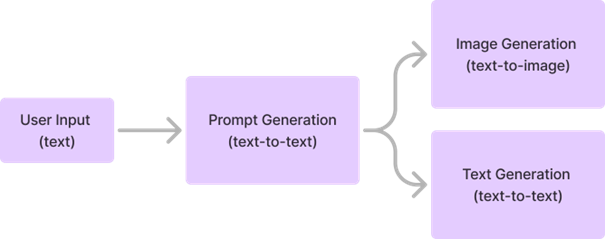
\includegraphics[width=\textwidth]{abbildungen/Process_image_generation}
    \caption{Prozess zur KI gestützten Social Media Content Generierung}
    \label{fig:process_content_generation}
\end{figure}


Der Anwender startet den Prozess mit der Angabe von Informationen über das gewünschte Produkt, für welches der Social Media Content generiert werden soll.
Im ersten Verarbeitungsschritt wird diese Informationen von einem Text-to-Text Machine Learning Modell verarbeitet, um daraus einen prompt zu generieren, welcher als Basis dient, um die finalen Social Media Inhalte zu generieren.
Entscheidend ist hierbei die Erweiterung der Produktangaben um stilistische Anweisungen und werbespezifischen Details, um ein möglichst engagement förderndes Ergebnis zu erzielen.
Der finalisierte Prompt, welcher als Basis für die Generierung von Bild und Text dient, wird anschließend einerseits ein weiteres Mal in ein Text-to-Text Machine Learning Modell übergeben, um daraus eine aussagekräftige Social Media Beschreibung in Textform zu generieren und andererseits in ein Text-to-Image Modell, um ein ansprechendes Bild zu generieren, welches für die Bewerbung des gewünschten Produktes geeignet ist.
Zur Auswahl eines geeigneten Text-to-Image Modelles wurden die beschriebenen Bewertungskriterien herangezogen um eine einheitliche Vergleichsbasis zu schaffen.
Die bewerteten Modelle basieren hierbei auf den populärsten Modellen der Machine Learning Plattform Hugging Faces.

Verglichen wurden unter anderem bekannte Modelle von etablierten Unternehmen wie die stable-diffusion modelle der Firma stability AI oder FLUX Modelle der firma black forest labs.
Um die leistungsfähigkeit der Modelle zu vergleichen und anschließend eine finale Auswahl je Modellziel treffen zu können, wurde ein prompt mit der Anweisung zur Generierung eines Döner Kebabs den verschiedenen Modelle als input übergeben.
Anschließend wurde die benötigte Zeit zur Generierung des outputs, sowie der output selbst miteinander verglichen.

Abbildung \ref{fig:results_image_generation} zeigt eine Zusammenfassung der generierten Inhalte in der Kategorie Text-to-Image.
Positiv zu bewerten ist, dass alle der getesteten Modelle den Auftrag korrekt interpretiert haben und eine Detailaufnahme des geforderten Produktes erzeugt haben.
Unterschiede gibt es jedoch im erreichten Realismus der Produktbilder.
Die FLUX modelle erzeugten hierbei die qualitativ hochwertigsten und realistischsten Bilder, die kaum von realen Produktbildern zu unterscheiden sind.
Die Stable Diffusion Modelle waren ebenfalls dazu fähig, inhaltlich korrekte aber dennoch minderwertige Produktbilder zu generieren.
Bei näherer Betrachtung der abgebildeten Zutaten eine gewisse Künstlichkeit auf, die Rückschlüsse auf KI generierte Inhalte schließen lässt.
Zudem erzeugen die Produktbilder nur mäßiges Interesse am Produkt, aufgrund der vergleichsweisen schlechten Komposition und stilistischen Umsetzung des Bildes.
Das Sana-\_1600M\_1024px Modell erzeugte ein ähnlich gelungenes, visuell ansprechendes Produktbild, wie die Modelle FLUX.1-dev und FLUX.1-schnell, dennoch ist der Realismusgrad deutlich schlechter, da sich die Strukturen der abgebildeten Zutaten leicht von den Originalen unterscheiden.

\begin{figure}[htbp]
    \centering
    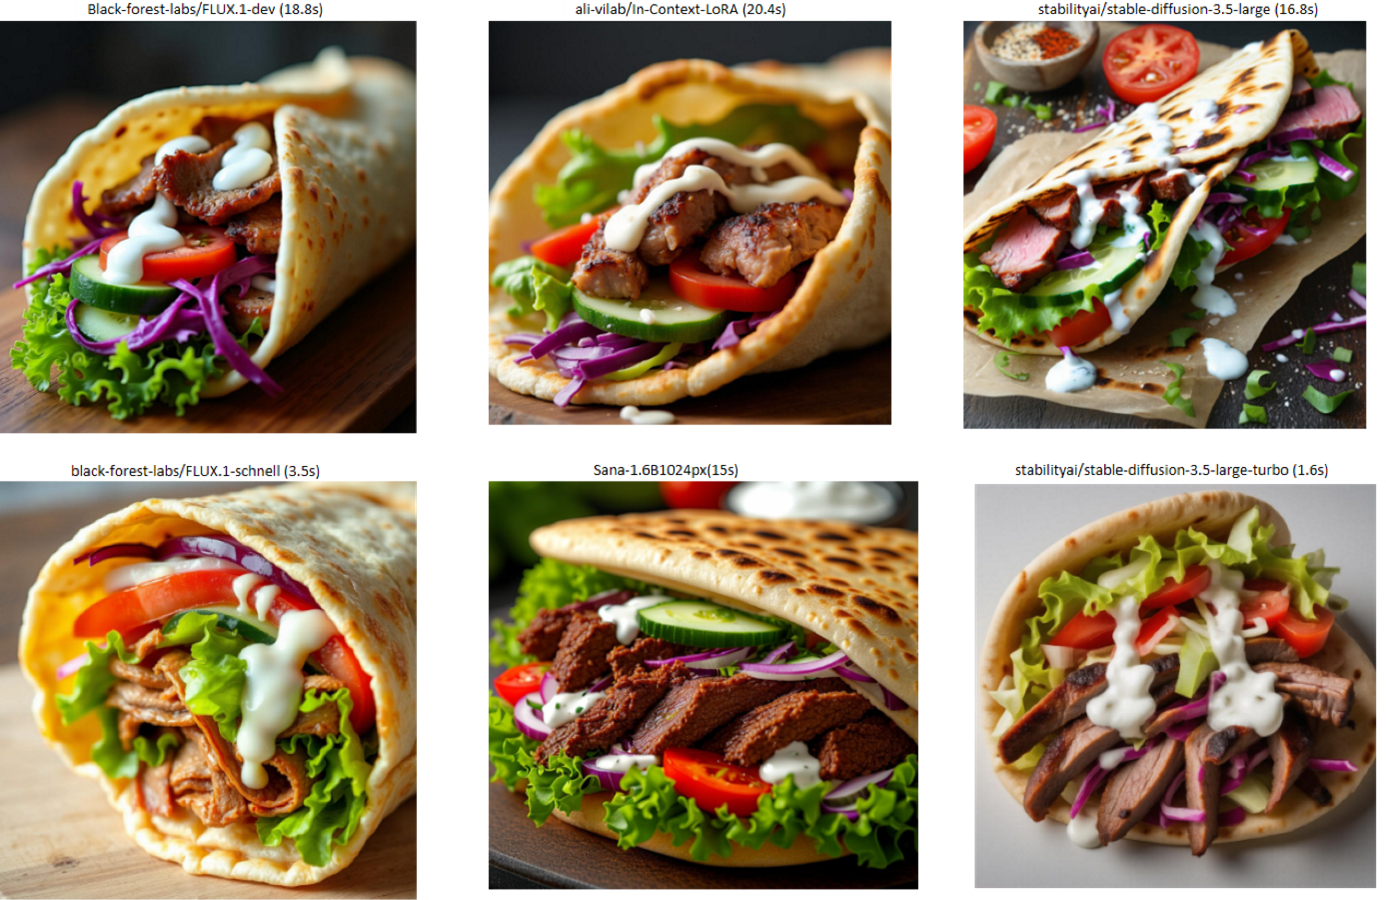
\includegraphics[width=\textwidth]{abbildungen/Results_image_generation}
    \caption{Vergleich der generierten Bilddateien durch die Text-to-Image Modelle}
    \label{fig:results_image_generation}
\end{figure}

Die Abbildungen \ref{fig:textresult_gemini} bis \ref{fig:textresult_nvdia_nemotron} bieten eine Zusammenfassung der generierten Inhalte zum Modellziel Text-to-Text mit den für Werbezwecken einsetzbaren Bildbeschreibungen.
Positiv zu bewerten ist der über alle Modelle hinweg erreichte Realismusgrad.
Jedes der getesteten Modelle erzeugte kurze, aussagekräftige, bildhafte und mit Schlagwörtern gefüllte Texte und baute zudem themenspezifische Hashtags ein.
Keine der generierten Bildbeschreibungen unterscheidet sich stark in Form und Inhalt von heutzutage gängigen Werbebeiträgen in sozialen Medien.
Hierbei auffällig ist, dass sowohl das QwQ-32B-Preview Modell, als auch das Llama-3.1-Nemotron-70B-Instruct-HF standardmäßig keine Emojis als stilistisches Mittel in den generierten Texten verwenden.
Darüber hinaus ist zu beobachten, dass das Llama-3.1-Nemotron-70B-Instruct-HF fiktive Rabattaktionen bewirbt, die nicht im Eingabeprompt gefordert waren.
Alle der untersuchten Text-to-Text Modelle, ausgenommen dem Mistral-7B-Instruct-v0.3 Modell, generierten zudem mehr als eine Bildbeschreibung, obwohl dies nicht im Eingabeprompt verlangt wurde.

\clearpage

\begin{figure}[htbp]
    \centering
    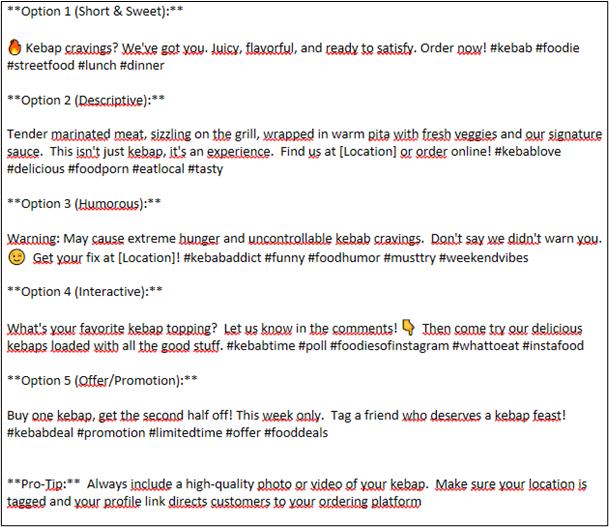
\includegraphics[width=\textwidth]{abbildungen/textresult_gemini}
    \caption{generierter Text durch das Text-to-Text Modell gemini-1.5-pro}
    \label{fig:textresult_gemini}
\end{figure}

\clearpage

\begin{figure}[htbp]
    \centering
    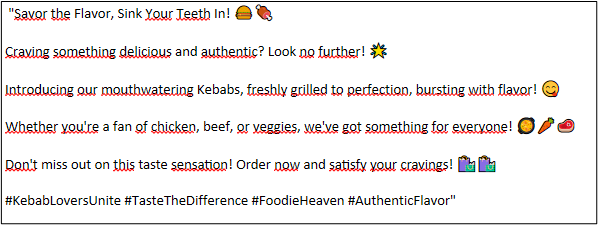
\includegraphics[width=\textwidth]{abbildungen/textresult_mistral}
    \caption{generierter Text durch das Text-to-Text Modell mistralai/Mistral-7B-Instruct-v0.3}
    \label{fig:textresult_mistral}
\end{figure}

\begin{figure}[htbp]
    \centering
    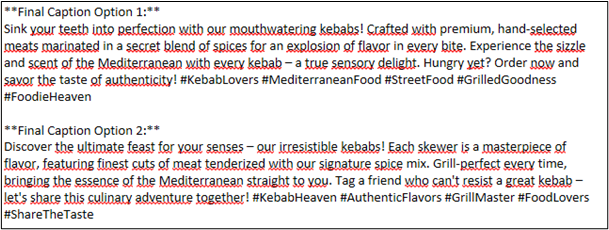
\includegraphics[width=\textwidth]{abbildungen/textresult_Qwen}
    \caption{generierter Text durch das Text-to-Text Modell Qwen/QwQ-32B-Preview}
    \label{fig:textresult_Qwen}
\end{figure}

\clearpage

\begin{figure}[htbp]
    \centering
    
\includegraphics[width=\textwidth]{abbildungen/textresult_nvdia_nemotron}
    \caption{generierter Text durch das Text-to-Text Modell nvidia/Llama-3.1-Nemotron-70B-Instruct-HF}
    \label{fig:textresult_nvdia_nemotron}
\end{figure}

Tabelle \ref{tab:table_modellvergleich} zeigt eine Zusammenfassung der erfassten Kennzahlen über alle untersuchten Modelle.
Auffällig ist jedoch, dass die untersuchten Machine Learning Modelle mit dem Modellziel Text-to-Text, trotz ihrer unterschiedlichen Größe und Trainingsdaten, in der Generierungsdauer und Qualität der Ergebnisse kaum voneinander abweichen.
Die Modellgröße unterscheidet sich jedoch erheblich, wobei das gemini-1.5-pro Modell mit über 100GB das größte Modell, und das Mistral-7B-Instruct-v0.3 mit 15.5GB das kleinste Modell darstellt.
Aus Effizienzgründen ist das Mistral-7B-Instruct-v0.3 Modell für die Kategorie Text-to-Text, welches die qualitativ hochwertigsten Ergebnisse in kürzester Zeit generierte, zu bevorzugen.

Die untersuchten Modelle in der Kategorie Text-to-Image hingegen, zeigen deutliche Unterschiede in der Qualität der generierten Inhalte, wobei die FLUX Modelle die qualitativ hochwertigsten Ergebnisse erzielen.
Im direkten Vergleich erzielte hierbei das FLUX.1-schnell Modell die besten Ergebnisse, da es die qualitativ hochwertigsten Bilder in kürzester Zeit generierte und somit zu bevorzugen ist.

\begin{table}[t]
  \centering
  \begin{tabular}{|p{3cm}|p{3cm}|p{2cm}|p{2cm}|p{3cm}|}
      \hline
      \textbf{Modellname} & \textbf{Modellziel} & \textbf{Modellgröße} & \textbf{Generierungsdauer} & \textbf{Qualität}\\ \hline
      {Black-forest-labs/FLUX.1-dev} & Text-to-Image & 23.8 GB & 18.8s & sehr gut\\ \hline
      {Black-forest-labs/FLUX.1-schnell} & Text-to-Image & 23.8 GB & \textless 5s & sehr gut\\ \hline
      {Efficient-Large-Model/Sana-\_1600M\_1024px} & Text-to-Image & 6.43 GB & \textless 5s & gut\\ \hline
      {Stabilityai/stable-diffusion-3.5-large} & Text-to-Image & 16.5 GB & 16.8s & befriedigend\\ \hline
      {Stabilityai/stable-diffusion-3.5-large-turbo} & Text-to-Image & 16.5 GB & 1.6s & ausreichend\\ \hline
      {Stabilityai/stable-diffusion-3.5-large} & Text-to-Image & 16.5 GB & 1.6s& befriedigend\\ \hline
      {Qwen/QwQ-32B-Preview} & Text-to-Text & \textgreater 50GB & 8s & sehr gut\\ \hline
      {gemini-1.5-pro} & Text-to-Text & \textgreater 100GB & 10s & sehr gut\\ \hline
      {mistralai/Mistral-7B-Instruct-v0.3} & Text-to-Text & 15.5 GB & \textgreater5s & sehr gut\\ \hline
  \end{tabular}
  \caption{Vergleich der generativen Machine Learning Modelle}\label{tab:table_modellvergleich}
\end{table}

\clearpage

\subsection{Auswahlprozess Web-Technologien}
Um geeignete Technologien für die Entwicklung der Applikation zu finden, wird ein Auswahlprozess durchgeführt.

Dieser Prozess folgt dem Konzept der PAPRIKA Methode von Hansen und Ombler.
Zu Beginn wird eine Liste von Kriterien erstellt, die für die Auswahl der Technologien relevant sind.
Anschließend wird eine Gewichtung der Kriterien vorgenommen, um die Relevanz der einzelnen Kriterien zu bestimmen.
Nachdem die Kriterien festgelegt sind, werden die zu vergleichenden Technologien identifiziert.
Abschließend erfolgt die Bewertung der Technologien anhand der Kriterien, indem Diese paarweise miteinander verglichen werden.
Dadurch wird für jede benötigte Komponente die am besten geeignete Technologie identifiziert.\footcite{Paprika2008}

Folgende Anforderungen wurden zur Bewertung der einzelnen Technologien identifiziert:

\begin{table}[htbp]
  \centering
  \begin{tabular}{|p{2cm}|c|p{5cm}|p{4cm}|}
      \hline
      \textbf{Kriterium} & \textbf{Gewicht} & \textbf{Beschreibung} & \textbf{Skala}\\ \hline
      {Lernkurve} & 0.4 & Lernaufwand in Relation zum Erfolgsgrad im Hinblick auf umzusetzende Features & flach, moderat, steil\\ \hline
      {Community} & 0.3 & Größe und Aktivität der Community sowie vorhandenes Lernmaterial & klein, mittel, groß\\ \hline
      {Bibliotheken} & 0.2 & Verfügbarkeit von Bibliotheken & begrenzt, mittel, umfangreich\\ \hline
      {Relevanz} & 0.1 & Aktualität und Weiterentwicklung der Technologie & niedrig, mittel, hoch\\ \hline
  \end{tabular}
  \caption{Bewertung der Anforderungen an Web-Technologien}\label{tab:table}
\end{table}

Im nächsten Schritt werden die zu vergleichenden Technologien identifiziert.
Folgende Komponenten werden für die Entwicklung der Applikation benötigt:

\begin{itemize}
  \item Frontend-Framework
  \item Backend-Framework
  \item Datenbank
\end{itemize}

Um den Auswahlprozess zu vereinfachen, wird die Auswahl auf drei Technologien je Kategorie beschränkt.
Dabei erfolgt die Auswahl anhand von bereits vorhandenem Wissen und Erfahrungswerten.
Es wurden folgende Technologien für die Auswahl identifiziert:

\begin{table}[htbp]
  \centering
  \begin{tabular}{|l|c|c|c|}
      \hline
      \textbf{Technologie Kategorie} & \textbf{Top 1} & \textbf{Top 2} & \textbf{Top 3} \\ \hline
      {Frontend-Framework} & Angular & VueJS & React \\ \hline
      {Backend-Framework} & Flask & Django & Cherrypy \\ \hline
      {Datenbank} & PostgreSQL & MySQL & MongoDB \\ \hline
  \end{tabular}
  \caption{Technologieauswahl Übersicht}\label{tab:Technologieauswahl Übersicht}
\end{table}

Zur Bestimmung der einzelnen Werte werden unterschiedliche Datenquellen herangezogen.
Zur Überprüfung der Relevanz wird die aktuelle Stackoverflow Developer Survey 2024\footcite{StackOverflow2024}, sowie State of JS 2023\footcite{stateofjsStateJavaScript2023} herangezogen.

Zusätzlich werden die Plattformen Github.com und Stackoverflow.com untersucht, inwiefern die Technologien dort vertreten sind.
Für die Frontend Frameworks im Speziellen werden die verfügbaren Libraries im Node Package Manager (NPM) untersucht.

Aus der Analyse lassen sich folgende Daten ableiten:

\begin{table}[h!]
    \centering
    \begin{tabular}{|l|p{2cm}|p{3cm}|p{3cm}|p{3cm}|}
        \hline
        \rowcolor{lightgray} Name & \textbf{Datum Veröffentlichung} & \textbf{Aktive Fragen auf Stackoverflow} & \textbf{Repositories auf Github mit Tag} & \textbf{Abhängigkeiten NPM} \\ \hline
        Angular & 2010\footcite{githubAngularReleaseV090} & 306.845 & 57.588 & 14.607 \\ \hline
        VueJS & 2014\footcite{eggheadEvanYou} & 108.341 & 26.600 & 80.824 \\ \hline
        React & 2013\footcite{githubReactCHANGELOG} & 481.823 & 173.000 & 240.000 \\ \hline
        \hline
        Flask & 2010\footcite{pypiFlask} & 55.856 & 50.985 & - \\ \hline
        Django & 2005\footcite{pypiDjango} & 313.041 & 67.366 & - \\ \hline
        Cherrypy & 2004\footcite{pypiCherryPy} & 1.370 & 147 & - \\ \hline
        \hline
        PostgreSQL & 1996\footcite{postgresqlHappyBirthday} & 178.607 & 56.562 & - \\ \hline
        MySQL & 1995\footcite{amazonWhatMySQL} & 661.661 & 75.826 & - \\ \hline
        Mongodb & 2009\footcite{mongodbMongoDBEvolved} & 176.192 & 111.693 & - \\ \hline
    \end{tabular}
    \caption{Bewertung von Technologien}\label{tab:Analyseergebnise Relevanz der Plattformen}
\end{table}

Darüber hinaus können die Ergebnisse der Studie von Bielek et al. herangezogen werden, welche Aufschluss über die Performance der einzelnen Technologien geben.
Aus der Untersuchung geht hervor, dass VueJS das effizienteste Frontend-Framework ist, gleichzeitig die niedrigste Anzahl an benötigten Programmcodes aufweist.\footcite{Bielak_2022}

Diese Erkenntnisse werden in der Untersuchung von Lipski et al. bestätigt.
Darüber hinaus wird in dieser Studie beschrieben, dass VueJS besonders für Entwickler ohne bisherige Erfahrung in der Webentwicklung geeignet ist.\footcite{Lipski_2021}

Diese Erkenntnisse wirkt sich positiv auf Lernkurve, wie auch die Relevanz der Technologie aus.
Die Syntax von VueJS bricht komplexe Zusammenhänge in einfachere Teile herunter, wodurch die Einarbeitung in die Technologie erleichtert wird.
Dadurch können gleiche Funktionen einfacher und schneller implementiert werden.

Auf Basis der gesammelten Daten und geleisteten Recherchen lassen sich die Technologien wie folgt bewerten:

\begin{table}[h!]
    \centering
    \begin{tabular}{|l|l|c|c|c|c|}
        \hline
        \rowcolor{lightgray} \textbf{Technologie} & \textbf{Kategorie} & \textbf{Community} & \textbf{Lernkurve} & \textbf{Bibliotheken} & \textbf{Relevanz} \\ \hline
        Angular & Backend Framework & \cellcolor{green!70}3 & \cellcolor{red!70}1 & \cellcolor{green!70}3 & \cellcolor{orange!70}2 \\ \hline
        VueJS & Backend Framework & \cellcolor{green!70}3 & \cellcolor{green!70}3 & \cellcolor{orange!70}2 & \cellcolor{green!70}3 \\ \hline
        React & Backend Framework & \cellcolor{green!70}3 & \cellcolor{orange!70}2 & \cellcolor{green!70}3 & \cellcolor{green!70}3 \\ \hline
        Flask & Frontend Framework & \cellcolor{orange!70}2 & \cellcolor{green!70}3 & \cellcolor{orange!70}2 & \cellcolor{orange!70}2 \\ \hline
        Django & Frontend Framework & \cellcolor{green!70}3 & \cellcolor{red!70}1 & \cellcolor{green!70}3 & \cellcolor{green!70}3 \\ \hline
        Cherrypy & Frontend Framework & \cellcolor{red!70}1 & \cellcolor{orange!70}2 & \cellcolor{red!70}1 & \cellcolor{red!70}1 \\ \hline
        PostgreSQL & Datenbank & \cellcolor{green!70}3 & \cellcolor{orange!70}2 & \cellcolor{green!70}3 & \cellcolor{green!70}3 \\ \hline
        MySQL & Datenbank & \cellcolor{green!70}3 & \cellcolor{green!70}3 & \cellcolor{orange!70}2 & \cellcolor{orange!70}2 \\ \hline
        Mongodb & Datenbank & \cellcolor{green!70}3 & \cellcolor{orange!70}2 & \cellcolor{green!70}3 & \cellcolor{green!70}3 \\ \hline
    \end{tabular}
    \caption{Bewertung von Technologien}\label{tab:Tabelle Bewertung von Technologien}
\end{table}

Zuletzt werden die jeweiligen Technologien paarweise miteinander verglichen.
Dabei wird die Bewertung der einzelnen Kriterien in Relation zueinander gesetzt, um die am besten geeignete Technologie zu identifizieren.
Neben den erhobenen Daten fließen auch subjektive Einschätzungen in die Bewertung mit ein.

\textbf{Frontend-Framework:}

Angular und VueJS sind beide als Webtechnologie etabliert und weisen eine entsprechende Community auf.
Ebenso gibt es für beide Tools zahlreiche Communities, wobei sich Angular dort besonders hervortut.
Für die Relevanz der Technologien erscheint VueJS jedoch vielversprechender.
Der entscheidende Faktor in diesem Vergleich ist die Lernkurve der Technologien, bei welcher VueJS mit einer flachen Einstiegserfahrung überzeugt.
Daher fiel die Entscheidung auf VueJS.

Beim Vergleich von Angular und React zeigt sich, dass React ebenfalls äußerst etabliert ist und als eines der beliebtesten Frontend-Frameworks gilt.
Der Umfang an verfügbaren Bibliotheken ist mit Angular vergleichbar.
Jedoch ist die Lernkurve von React im Vergleich zu Angular einfacher, was zu einer Entscheidung zugunsten von React führte.

Der Vergleich von VueJS und React zeigt, dass beide Technologien im Hinblick auf die Community gleichauf sind.
Das Angebot an Bibliotheken ist für React dennoch größer.
Beide Frameworks gelten als äußerst relevant für moderne Applikationen.
Entscheidender Faktor im Vergleich ist die Lernkurve, bei welcher VueJS mit einer flachen Einstiegserfahrung überzeugt.
Aus diesem Grund fiel die Wahl auf VueJS.

In der gesamten Betrachtung der Frontend-Frameworks ist VueJS die Technologie, die am besten zu den Anforderungen passt.

\textbf{Backend-Framework:}

Flask und Django stellen die beiden beliebtesten Python-Frameworks zur Entwicklung von Webapplikationen dar, wobei Django die größere Community aufweist.
Daraus resultiert ein größeres Angebot an Bibliotheken für Django im Vergleich zu Flask.
Ebenso die Relevanz der Technologie ist für Django höher einzustufen.
Über die Lernkurve lässt sich sagen, dass Flask eine flachere Lernkurve aufweist als Django, welches eher als steil zu bewerten ist.
Im direkten Vergleich ist jedoch der Lernaufwand für Django gerechtfertigt, da die Technologie eine Vielzahl an Features bietet und durch die große Community und dem Angebot an Bibliotheken unterstützt wird.
Dadurch ist die Entscheidung auf Django gefallen.

Der Vergleich von Flask und Cherrypy zeigt, dass Flask in allen betrachteten Kriterien besser abschneidet.
Die Community ist größer, das Angebot an Bibliotheken umfangreicher und die Relevanz höher einzustufen.
Auch die Lernkurve wird flacher gewertet als bei Cherrypy, wodurch die Entscheidung, im direkten Vergleich, auf Flask fällt.

Django ist, ebenso wie Flask, in fast allen Kriterien besser zu bewerten als Cherrypy.
Einzig die Lernkurve ist bei Cherrypy flacher einzustufen.
Dennoch überzeugt Django durch die größere Community, das umfangreichere Angebot an Bibliotheken und die höhere Relevanz, weswegen die Entscheidung auf Django fällt.

In der gesamten Betrachtung der Backend-Frameworks ist Django die Technologie, die am besten zu den Anforderungen passt.

\textbf{Datenbanken:}

PostgreSQL und MySQL sind beide als relationale Datenbanken etabliert und weisen eine entsprechende Community auf.
Dabei gilt MySQL als die einsteigerfreundlichere Datenbank während PostgreSQL eine weitere Verbreitung in der gegenwärtigen Technologielandschaft aufweist.
Zudem gilt PostGreSQL als die relevantere Technologie.
Aufgrund der zuvor abgestimmten Gewichtung der Kriterien fällt die Entscheidung auf MySQL.

Der Vergleich von PostgreSQL und MongoDB zeigt, dass die betrachteten Merkmale in etwa gleich zu bewerten sind.
Zentraler Unterschied zwischen beiden Technologien ist die Art der Datenbank, wobei PostgreSQL als relationale Datenbank und MongoDB als NoSQL-Datenbank klassifiziert wird.

Für die Entscheidung über die Datenbanktechnologie wird PostgreSQL als SQL bzw. MongoDB als NoSQL Variante gewählt.
Im Rahmen der Architekturkonzipierung können beide Technologien in Betracht gezogen werden, wobei die Entscheidung auf Basis der spezifischen Anforderungen der Applikation getroffen wird.




\newpage
\section{Beratender Teil} \label{sec:beratender-teil}

\subsection{Essenzielle Eigenschaften bei Social Media Posts}
Social-Media-Posts bilden das Herzstück einer jeden Social-Media-Plattform.
Dabei können sich, je nach Plattform, die Social Media Beiträge merkbar unterschieden.
So setzt Instagram, als ausgewählte Social-Media-Plattform, ausschließlich den Schwerpunkt auf visuelle Beiträge, welche i. d. R. aus einem Foto oder (Kurz-) Video und einem Text unter dem visuellen Element bestehen.
Damit ein Beitrag auf einer Social-Media-Plattform gut ankommt und Klicks generiert, gibt es einige Kriterien die zu beachten sind, bzw. Eigenschaften die zu erfüllen sind.

Das erste Kriterium beschreibt die Kreativität und die Einzigartigkeit von Beiträgen.\footcite{kaplan_users_2010,keller_building_1993}
Dabei geht es inhaltlich darum, dass besonders auffällige Beiträge, im Sinne der Authentizität, Ausgefallenheit, oder Individualität eher bei Benutzern der Plattform auf Interesse stoßen als Beiträge, die sich nicht von der Masse abheben.
Ein Beispiel hierfür ist die Abbildung des traditionellen Zubereitungsprozesses einer Pizza, die mit einer besonderen Tomatensauce sowohl visuell als auch schriftlich beworben wird.\footcite{green_role_2000}

Ein weiteres Kriterium ist die Definition einer Zielgruppe.\footcite{kotler_marketing_management}
Dies ist erheblich wichtig, da mit der Auswahl einer Zielgruppe entsprechende gewählte Artikulation notwendig ist.
Ebenso wirkt sich das auf den Stil der Beiträge aus.
Ein italienisches Restaurant, das sich durch verschiedene Faktoren wie eine lockere Atmosphäre, günstige Preise und spezielle Angebote an eine junge Zielgruppe wendet, legt dabei visuell als auch sprachlich andere Schwerpunkte bei den Beiträgen als ein vergleichbares Restaurant, das auf eine Zielgruppe mit gesteigerter Kaufkraft ausgerichtet ist.

Social-Media-Beiträge, aus Sicht eines Gastronomen, sollten immer eine Konversionsorientierung haben.\footcite{website_quality_customer_satisfaction}
Genauer gesagt, definiert die Konversionsorientierung ein Call-to-Action, bei dem der Kunde kommunikativ aufgefordert wird auf einen Link zu klicken, ein Tisch zu reservieren oder vergleichbare interaktionen zu tätigen.
Eine Strategie, die das Call-to-Action Prinzip verstärkt ist die Verlustaversion, im Sinne von Marketingkampagnen, die auf ein zeitlich, oder physisch begrenztes Angebot hinweisen.\footcite{jstor_example}
Ein Beispiel für diese Eigenschaft wäre das Bewerben eines zeitlich begrenzten Angebotes von drei Pizzen im Preis von zwei Pizzen.

Ansprechende Bildbeiträge spiegeln ein weiteres, wichtiges Kriterium wider, um die Aufmerksamkeit von Nutzern zu erlangen.\footcite{davidson_social_media}
So geht aus einer Studie von Sabate et al. aus dem Jahr 2014 hervor, dass visuelle Inhalte weitaus mehr Engagement erzeugen, als rein auf Text basierte.
Dabei sollten die Bilder auch aussagekräftig sein und mit der Eigenschaft der Kreativität und Einzigartigkeit synergieren.\footcite{sabate_factors}

Die persönliche und emotionale Ansprache der Zielgruppe und das Erzählen einer Geschichte sind bei dem Social-Media-Marketing ebenfalls wichtige Eigenschaften, die in Beiträgen beachtet werden sollten.
Gemeint sind dabei Inhalte, die Emotionen, wie z. B. Vorfreude, oder Hunger, bei den Social Media Nutzern auslösen.
Erzählungen über das Team, die Philosophie, die Geschichte des Restaurants, oder die Besonderheit der Zutaten sind hier wichtige Aspekte in der Kommunikation mit den Kunden auf den Social-Media-Plattformen, um diese als Kunden zu gewinnen.\footcite{book}

Zwei weitere Aspekte, die ebenfalls großen Einfluss auf das Social-Media-Marketing nehmen, sind zu einem der Ereignisbezug und zum anderen der Trendbezug.
Dabei beziehen sich diese beiden Punkte auf Aspekte, die einen Bezug zur aktuellen Saison, wie beispielsweise in Form der Jahreszeiten, oder zu gegenwärtigen Ereignissen, wie etwa einer Fußball-Weltmeisterschaft, herstellen.
Der Bezug auf solche Aspekte führt generell zu einem höheren Engagement.
Ein Beispiel für einen saisonalen Bezug wäre die Bewerbung einer besonderen Pizza, die nur während der Wintersaison erhältlich ist.
Ein weiteres Beispiel für den Trendbezug wäre die Reaktion auf die Ergebnisse der deutschen Nationalmannschaft, bei der aus Fußballspielsiegen Rabatte für Pizzabestellungen resultieren.\footcite{inbook}

Eine weitere, essenzielle Eigenschaft spiegelt die auf Social Media ausgerichtete Optimierung der Inhalte wider.
Diese Eigenschaft behandelt Hashtag-Strategien, welche relevant sind für die Auffindbarkeit der Social-Media-Beiträge, und wie die Strukturierung der Inhalte zu erfolgen hat, um vom Social-Media-Algorithmus bevorzugt angezeigt zu werden.\footcite{social_media_marketing}

Darüber hinaus sollte bei jedem Social Media Beitrag die Mehrsprachigkeit und Lokalität betrachtet werden.
Beide Aspekte zielen auf ein höheres Engagement.
Durch den möglichen Einsatz von Mehrsprachigkeit, wie z. B. neben der deutschen Sprache auch noch die englische Sprache, und den Bezug auf die Lokalität, wie z. B. auf lokale Sport Events oder kulturelle Besonderheiten, kann eine höhere Zielgruppe angesprochen werden, was wiederum zu einer höheren Nachfrage führen würde.\footcite{global_marketing_advertising}

Zusammengefasst wurden folgende Eigenschaften betrachtet und als relevant für Social Media Beiträge designiert: „Kreativität“, Einzigartigkeit, „Zielgruppenorientierung“, Konversionsorientierung“, „Bildbeiträge“, „persönliche und emotionale Ansprache“, „Story telling“, „Ereignis- und Trendbezug“, „Social-Media-Optimierung“, „Strukturierung der Posts“, „Mehrsprachigkeit“ und „Lokalität“.
Diese Eigenschaften werden als fundierte Basis für die Entwicklung und Optimierung der Prompt des LLMs bezogen.

\subsection{Entwicklung eines Erstenwurfs für das Applikationsdesign}\label{subsec:entwicklung-eines-erstenwurfs-fuer-das-applikationsdesign}
In diesem Kapitel wird der Erstentwurf für das Applikationsdesign vorgestellt.
Der Erstentwurf beschreibt sowohl die Frontend- als auch die Backend-Architektur der Applikation.

\textbf{Frontend}\newline
Das Frontend stellt den Interaktionsbereich für den Benutzer dar.
Entsprechend ist es wichtig, dass das Frontend übersichtlich und intuitiv gestaltet ist.
Dabei ist es entscheidend, die komplexen Zusammenhänge der Applikation und abgebildeten Prozesse so zu visualisieren, dass der Benutzer nicht überfordert wird.
Die gesamte \ac{UX} soll so gestaltet sein, dass der Benutzer durch die Applikation geführt und dadurch die Akzeptanz der Applikation erhöht wird.

Zusätzlich soll sich die Applikation an die Corporate Identity des Unternehmens anpassen.
Dies soll durch die Verwendung der Unternehmensfarben in der Applikation und des Logos erreicht werden.

Zur Umsetzung gilt folgendes zu beachten:
\begin{itemize}
    \item Das DISH POS typische Orange soll als primäre Farbe verwendet werden.
    \item Als sekundäre Farben sollen Grau- und Blautöne verwendet werden.
    \item Die Farben sollen so gewählt werden, dass sie die Aufmerksamkeit des Benutzers auf wichtige Elemente lenken.
    \item Unternehmens- und Applikationslogos müssen an strategischen Stellen platziert werden.
\end{itemize}
\newpage

Aus den genannten Anforderungen wurden folgende Design-Elemente abgeleitet:

\textbf{Landing Page Darstellung und wiederkehrende Elemente}\newline
Das Konzept zur Landing Page besteht aus mehreren runden Interaktionselementen (Bubbles), welche die verschiedenen Funktionen der Applikation repräsentieren.
Dabei werden die wichtigen Funktionen, wie z. B. die Generierung von Social-Media-Content, durch eine größere Bubble hervorgehoben.
Durch den Größenunterschied der Bubbles kann die Prominenz der Funktionen visualisiert werden.
Als zentrales, wiederkehrendes Element über alle Seiten hinweg, wird eine Textausgabe zentral platziert, welche den Benutzer durch die Applikation führt.
Diese Textausgabe fungiert dabei als interaktive Komponente, die dem Benutzer ein personalisiertes Erlebnis bietet.
Der Navigationsbereich wird als Sidebar auf der linken Seite platziert, erreichbar über ein Burger-Icon.
Wie im \ac{UX} Design vorgesehen, wird das DISH POS Logo daneben platziert, wodurch es ein strategisch platziertes Element darstellt.
Zuletzt findet sich ein Login Icon in der oberen rechten Ecke, welches den Benutzer zum Login-Bereich führt.
Insgesamt ist die Darstellung minimalistisch gehalten, um den Benutzer auf die wichtigsten Elemente zu fokussieren.\footnote{Siehe Anhang, Abbildung \ref{fig:landing-page-concept}.}

Das aus dem Entwurf abgeleitete Design zeigt zusätzlich, dass durch entsprechende Farbgebung die Corporate Identity des Unternehmens eingebunden wird.\footnote{Siehe Anhang, Abbildung \ref{fig:landing-page}.}

\textbf{Dialog Darstellung}\newline
Die Dialog-Darstellung strukturiert sich durch ein zentrales Eingabefeld, in welchem der Benutzer durch einen geführten Dialog mehrere Fragen beantwortet.
Die dadurch gesammelten Eingaben werden später in der Generierung von Social-Media-Content verwendet, indem diese systematisch in die Prompts einfließen.
Das zentrale Textausgabeelement wird durch eine Fortschrittsanzeige ergänzt, welche den Benutzer über den aktuellen Stand des Dialogs informiert.
Dadurch wird erreicht, dass der Benutzer jederzeit über den Fortschritt informiert ist und dadurch die Akzeptanz der Applikation erhöht wird.
Nach dem Beantworten einer Frage wird der Benutzer durch eine Animation auf die nächste Frage hingewiesen.
Dadurch wird die minimalistische Darstellung der Anwendung beibehalten und eine übermäßige Informationsflut vermieden.\footnote{Siehe Anhang, Abbildung \ref{fig:dialog-concept}.}

Im detaillierten Design wird durch den Einsatz der DISH POS Farben die Benutzbarkeit weiter verstärkt.
Durch das Färben der weiterführenden Buttons in Orange bzw. das blaue Hervorheben für ein Navigieren in vorherige Schritte, wird eine wiederkehrende Designkomponente eingeführt.
Zudem wird durch das umgangssprachliche Formulieren, sowohl der Fragen als auch der Navigation, eine persönliche Ansprache an den Benutzer gewährleistet.
Ebenso findet sich die primäre orangene Farbe in der Fortschrittsleiste wieder, wodurch die Corporate Identity des Unternehmens eine strategische Position erfährt. \footnote{Siehe Anhang, Abbildung \ref{fig:dialog-page}.}

\textbf{Post Editor Darstellung}\newline
Der Post Editor stellt die komplexeste Komponente der Applikation dar.
Dieser gliedert sich in zwei Hauptbereiche, dem eigentlichen Editor und einer Vorschau der generierten Inhalte.
Der Editor ist dabei auf die minimalen Funktionen reduziert, um den Benutzer nicht zu überfordern.
Jede Eingabe ist dabei als eigenes Element dargestellt und beinhaltet die zuvor generierten Texte und Bilder.
Über den Editor kann der Nutzer die generierten Inhalte und Einstellungen anpassen, darunter den Zeitplan, den Text und das Bild.
Die Vorschau zeigt den geplanten Post im Design der Zielplattform, beispielsweise dargestellt für Instagram.\footnote{Siehe Anhang, Abbildung \ref{fig:editor-concept}.}

Im detaillierten Design wurden die DISH POS Farben in den Editor integriert, konsistent zu den bisherigen Darstellungen.
Abweichend vom initialen Konzept wurde zusätzlich ein Bereich für die Eingabe der Call-to-Action hinzugefügt.\footnote{Siehe Anhang, Abbildung \ref{fig:editor-page}.}

\textbf{Kalender Darstellung}\newline
Der Kalender erlaubt dem Nutzer die geplanten Posts zu verwalten und zu bearbeiten.
Dieser strukturiert sich Grundlegend durch eine Übersicht der aktuellen Woche, welche über eine Navigation durch die Wochen erweitert werden kann.
Jede Woche beinhaltet eine Kachel je Post, welche Information darüber enthält, wann der Post veröffentlicht wird und welcher Inhalt geplant ist.
Zudem ist für den User ersichtlich, auf welcher Plattform der Post veröffentlicht wurde.
Über Chips in der Fusszeile ist für den Nutzer transparent, ob ein Post veröffentlicht wurde, ob dieser geplant ist oder ob ein Entwurf vorliegt.
Dabei wird jeder Status in einer eigenen Farbe dargestellt, um einen schnellen Überblick zu gewährleisten.
Das zentrale Textausgabeelement wird in den oberen rechten Bereich verschoben, um den Fokus auf die Kalenderansicht zu legen, dabei jedoch weiterhin präsent zu sein.
Darüber werden dem Nutzer, in Anlehnung an die Landing Page, Bubbles mit den wichtigsten Funktionen der Kalenderansicht angezeigt.\footnote{Siehe Anhang, Abbildung \ref{fig:calendar-concept}.}

Abweichend zum Konzept wurde die Darstellung in der detaillierten Ansicht auf ein Icon für die Plattform reduziert.
Zudem wurde die Navigation durch den Kalender visuell reduziert, da davon auszugehen ist, dass nutzer selten weitreichende Zeiträume im Kalender betrachten werden.
Diese ist in der Standardansicht versteckt und wird über ein Hover-Element sichtbar.\footnote{Siehe Anhang, Abbildung \ref{fig:editor-page}.}

Als technische Basis für das Frontend wird, als Ergebnis der vorangegangenen Recherche, Vue.js verwendet.
Dieses wird zum Betrieb im Kubernetes Engine Cluster bereitgestellt.
Für den Betrieb im Kubernetes Cluster muss die Software Architektur Stateless sein, um mit der Skalierung kompatibel zu sein.
Eine Stateless-Architektur bedeutet, dass die Applikation keine Zustände speichert.
Würde die Applikation Zustände speichern, müssten diese bei einer Skalierung auf mehrere Instanzen synchronisiert werden, was zu einem erhöhten Aufwand führen würde.

Um die Applikation im Kubernetes Cluster hosten zu können, erfolgt das Verpacken der Vue.js Applikation in ein Docker-Image über den Google Cloud Build Service.\footcite{google_cloud_build}

Das daraus erzeugte Docker-Image wird in den Google Kubernetes Engine Cluster genutzt und entsprechend gestartet.
Dabei wird eine Deployment-Struktur, bestehend aus einem Load Balancer Service, sowie mindestens zwei Pods erstellt.
Der Load Balancer wird für externe Zugriffe konfiguriert und leitet die Anfragen an die Pods weiter.
Der Betrieb, mit mindestens zwei Pods, gewährleistet eine hohe Verfügbarkeit der Applikation und ermöglicht eine einfache Skalierung.
In der Entwicklungsphase ermöglicht der Multi-Pod-Betrieb ein frühes Testen von Load-Balancing und Skalierung, sowie die Überprüfung der Stateless-Architektur.

Zusätzlich enthält das Deployment sowohl Konfigurations- als auch Secrets-Dateien, um die Applikation zu konfigurieren und sensible Daten zu schützen.

\textbf{Backend}\newline
Ziel der Backend-Architektur ist es, die Datenhaltung und -verarbeitung zu gewährleisten und die benötigten Aufrufe zu anderen Komponenten zu ermöglichen.
Im Rahmen dieses Erstenwurfs wird zunächst ein einzelner Service konzipiert, der die Datenhaltung und -verarbeitung übernimmt, genannt \ac{SMC} Service

Der \ac{SMC} Service stellt eine \ac{REST} \ac{API} bereit, welche die Kommunikation mit dem Frontend ermöglicht.
Die \ac{REST} \ac{API} setzt sich aus verschiedenen Endpunkten zusammen, welche jeweils die verfügbaren Ressourcen und Aktionen beschreiben.

Folgende Ressourcen stellt der Service bereit:
\begin{itemize}
    \item \textbf{/generate-content} - POST: Dieser Endpunkt dient der generierung und Speicherung von Social-Media-Content.
    \item \textbf{/get-content} - GET: Dieser Endpunkt ermöglicht das Abrufen von generiertem Social-Media-Content.
\end{itemize}

Die implementierung des \ac{SMC} Services erfolgt über das Python Framework Django\footcite{djangoproject}.
Zur Kommunikation mit den Google Cloud Services wird die Google Cloud Python SDK\footcite{googlecloudpython} verwendet.

Mithilfe der Google Cloud Python \ac{SDK} und entsprechender Konfiguration des API Clients wird die Kommunikation mit den als Cloud Service gehosteten Text-to-Text- und Text-to-Image-Modellen ermöglicht.
Der POST Endpunkt wird vom Frontend aufgerufen, sobald der Benutzter seine Eingaben im Frontend abgeschlossen hat und den Social-Media-Content generieren möchte.
Anschließend werden die Eingabeparameter über ein \ac{HTTP} Request-Body Objekt im \ac{JSON} Format an den \ac{SMC} Service gesendet.
Dieser verarbeitet den Request und routet diesen an den zuständigen POST Endpunkt.
Über den POST Endpunkt wird anschließend durch Verwendung der Google Cloud \ac{REST} \ac{API} ein weiterer \ac{HTTP}-Request and den Text-to-Text-Modell Cloud Service gesendet.
Der Text-to-Text-Modell Cloud Service generiert anschließend aus den Eingaben einen finalen Eingabeprompt und sendet eine \ac{HTTP}-Response mit den Ergebnissen der Generierung als HTTP-Response Body, welche vom \ac{SMC} Service entgegengenommen und verarbeitet wird.
Der \ac{SMC} Service verwendet anschließend den finalen Eingabeprompt, und tätigt zwei weitere \ac{HTTP}-Requests, parametrisiert mit dem generierten Eingabeprompt, an den Text-to-Image-Modell Cloud Service und den Text-to-Text-Modell Cloud Service über die Google Cloud \ac{REST} \ac{API}, um die vom User geforderten Inhalte final zu generieren.
Die generierten Social-Media-Content Inhalte werden anschließend vom \ac{SMC} Service verarbeitet, über einen \ac{HTTP}-Request in der Datenbank gespeichert und via \ac{HTTP}-Response auf die initiale Anfrage an das Frontend zur Visualisierung zurückgegeben.

Der GET Endpunkt wird vom Frontend aufgerufen, sobald der Benutzer über die entsprechende Funktion im Frontend die Historie der generierten Inhalte einsehen möchte.
Hierzu greift der GET Endpunkt des \ac{SMC} Services über die Google Cloud \ac{API} an die konfigurierte Datenbank zu und gibt die gespeicherten Inhalte mithilfe einer Paginierungslogik an das Frontend per \ac{HTTP}-Response zurück.
Durch Ergänzung des Resource parameters kann der Benutzer zudem zwischen den verschiedenen Ressourcen, wie z. B. generierte Texte oder Bilder, wechseln.

Die Datenhaltung wird über eine Datenbank realisiert, welche innerhalb des Google Cloud Services betrieben wird.
Folgende Daten werden in der Datenbank gespeichert:
\begin{itemize}
    \item Prompts
    \item Antworten
    \item User-Feedback
    \item Generierte Bilder
    \item Sonstige Metadaten
\end{itemize}

Das Hosting des SCM Service erfolgt ebenfalls über den Google Kubernetes Engine Cluster.
Dabei ist das Kubernetes Deployment gleich aufgebaut wie das Frontend-Deployment.
Bei Bedarf können die Deployments unabhängig voneinander skaliert bzw. konfiguriert werden.

\textbf{Strategie zur Datenhaltung}\newline
Zum Speichern der textbasierten Daten kann entschieden werden, ob Cloud Spanner als relationale Datenbank oder Data Store als NoSQL-Datenbank verwendet wird.\footcite{google_spanner}\footcite{google_datastore}

Die Untersuchung von Khan et al. zeigt, dass sich der NoSQL-Ansatz besser dazu eignet, erste Prompts und deren Antworten zu speichern.
Durch die schemalose Struktur von NoSQL-Datenbanken können neue Prompts und Antworten einfach hinzugefügt werden, ohne dass die Datenbankstruktur angepasst werden muss.
Darüber hinaus lassen sich diese Technologien gut in die Google Cloud Services integrieren.
Der Einsatz von einer relationalen Datenbank bietet sich in einem nachgelagerten Schritt an, in welchem die gesammelten Daten analysiert, strukturiert und ausgewertet werden sollen.\footcite{Khan2022SQL}

Entsprechend wird für den produktiven Einsatz des Prototypen der Google Data Store Service betrachtet.
Zur lokalen Entwicklung wird entsprechend MongoDB eingesetzt, da dies der NoSQL Favorit aus der vorangegangenen Recherche ist.

\textbf{Speicherung von Bildern}\newline
Neben den textbasierten Daten müssen auch die generierten Bilder gespeichert werden.
Dadurch wird eine effiziente Speicherung und Verwaltung der generierten Bilder gewährleistet und ein wiederverwendbarer Zugriff auf die Bilder ermöglicht.
Zur Speicherung von Bildern wird Google Cloud Storage verwendet.
Google Cloud Storage ist ein skalierbarer und kostengünstiger Speicher, der eine einfache Verwaltung von Bildern ermöglicht.
In diesem Service wird ein Bucket erstellt, in dem die Bilder gespeichert werden.\footcite{google_storage}

Die Erzeugung der Bilder wird über den Social-Media-Campaign Service gestartet, indem das Text-to-Image-Modell aufgerufen wird.
Das Modell generiert das Bild und schickt es an den \ac{SMC} Service zurück.
Dieser speichert das Bild im Google Cloud Storage und persistiert den Pfad im Data Store.
Bei Abfragen des Bildes wird der Pfad aus dem Data Store gelesen und über die \ac{REST} \ac{API} an das Frontend zurückgegeben.

Für den Prototypen wird ein einfacher Mechanismus implementiert, der die Bilder direkt im Google Cloud Storage speichert und den Pfad im Data Store persistiert.
Dabei ist zu beachten, dass die Bilder in einem öffentlichen Bucket gespeichert werden, um den Zugriff für das Frontend zu ermöglichen.
Zusätzlich ist die Auslastung des Services im produktiven Einsatz zu beachten, da die Speicherung von Bildern einen hohen Speicherbedarf verursachen kann.

Als Lösung kann die Speicherung der Bilder durch eine Sidecar-Architektur ausgelagert werden, um die Last auf den \ac{SMC} Service zu reduzieren.
Dabei wird ein weiterer Service implementiert, der die Bilder entgegennimmt und im Google Cloud Storage speichert.
Dieser Service wird innerhalb des \ac{SMC} Deployments gestartet und übernimmt die Speicherung der Bilder.\footcite{microsoft_sidecar_pattern}

Dadurch entsteht der Vorteil, dass eine unabhängige Auswahl der Speicherungstechnologie für die Bilder getroffen werden kann, wodurch die Performance verbessert werden kann.
Darüber hinaus teilen sich alle Pods des Deployments den gleichen Lebenszyklus, was die Wartung und Skalierung vereinfacht.\footcite{kubernetes_sidecar_containers}

Um die Bilder über einen Pfad für das Frontend verfügbar zu machen, wird ein weiterer Service, das Google \ac{CDN}, verwendet.
Das CDN fungiert als Zwischenspeicher für statische Inhalte und stellt einen, gesondert skalierbaren, Zugriffspunkt für diese Daten bereit.\footcite{google_cloud_cdn_overview}
Dadurch wird sowohl die benötigte Bandbreite bei der Kommunikation mit den Applikationsservices reduziert, als auch die Ladezeiten für den Benutzer verkürzt.
Zudem reduzieren sich dadurch die Entwicklungs- und Wartungskosten, da besondere Encoding- und Skalierungsschritte entfallen.

Das \ac{CDN} wird so konfiguriert, dass es auf den angelegten Bucket im Google Cloud Storage zugreift und die Bilder an den Benutzer ausliefert.
Dabei werden Synergieeffekte genutzt, da das \ac{CDN} bereits in der Google Cloud integriert ist und somit eine einfache Konfiguration ermöglicht.

Die technische Architektur der Applikation kann wie folgt illustriert werden:

\begin{figure}[htbp]
    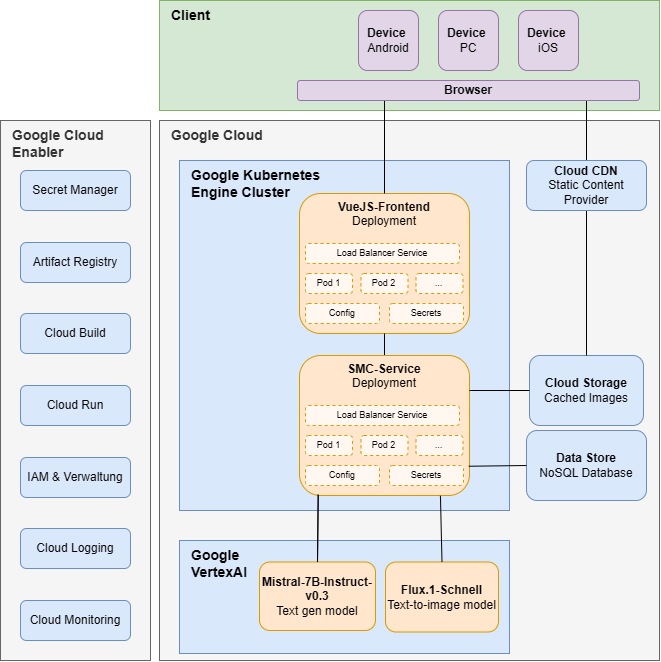
\includegraphics[width=0.8\textwidth]{abbildungen/Drawio/SystemArchitektur}
    \caption{Abbildung der Systemarchitektur}
    \label{fig:sytem-architektur}
    \raggedright Quelle: Eigene Darstellung
\end{figure}

\subsection{Antizipation der Kosten und des Nutzens}

Zur Berechnung der variablen Kosten im produktiven Betrieb der Plattform sind verschiedene Facetten zu betrachten, darunter die entstehenden Kosten für das Generieren und
speichern von Bild- und Textinhalten, die anfallenden Betriebskosten durch in Anspruchsnahme von Cloud Services sowie später anfallende Personalkosten für die Wartung und Weiterentwicklung der Plattform.

Um die Kostenstruktur der Plattform zu schätzen, werden verschiedene Szenarien betrachtet, welche die Kosten der Applikation unterschiedlich beeinflussen.
Dabei wird zwischen einem Best Case, einem Worst Case und einem realistischen Szenario unterschieden, welche sich maßgeblich durch die erwarten Nutzerzahlen unterscheiden.
Für die nachfolgende Kostenschätzung werden folgende Nutzerzahlen angenommen:

\begin{itemize}
    \item Best Case: 5000 User
    \item Worst Case: 50 User
    \item Realistisches Szenario: 500 User
\end{itemize}

\textbf{Generierung und Speicherung von Bildern}\newline
Zum Generieren der Bilder wird das Text-to-Image-Modell Flux-1-Schnell verwendet, welches auf der Google Cloud Plattform als Endpunkt bereitgestellt wird.
Dabei wird als Maschine ein in Belgien gehostetes n1-standard-4 gewählt, welches 4 vCPUs und 15 GB RAM besitzt.
Dies ist die kleinstmögliche Konfiguration für das Modell und verursacht Kosten von 0,24 USD pro aufgewendete Maschinenstunde.\footcite{GoogleVertexAI2025}

Im Testbetrieb des Prototypen lag die Inferenzzeit pro Anfrage bei ca. 500 ms.
Basierend auf den festgelegten Szenarien ergibt sich folgende Kostenstruktur, bei der Annahme, dass jeder User 10 Anfragen pro Monat stellt:

\begin{itemize}
    \item Best Case: 5000 User * 10 Anfragen * 0,5 s * 0,24 USD = 600 USD
    \item Worst Case: 50 User * 10 Anfragen * 0,5 s * 0,24 USD = 6 USD
    \item Realistisches Szenario: 500 User * 10 Anfragen * 0,5 s * 0,24 USD = 60 USD
\end{itemize}

Die generierten Bilder werden im Google Cloud Storage gespeichert.
Dieser wird in der Region Belgien gehostet und wird mit 0,02 USD pro GB und Monat berechnet.\footcite{GoogleCloudStorage2025}

Die im Testbetrieb erzeugten Bilder hatten eine Größe von ca. 128 KB.
Basierend auf den festgelegten Szenarien ergibt sich folgende Kostenstruktur:
\begin{itemize}
    \item Best Case: 5000 User * 10 Anfragen * 128 KB * 0,02 USD = 12,8 USD
    \item Worst Case: 50 User * 10 Anfragen * 128 KB * 0,02 USD = 0,128 USD
    \item Realistisches Szenario: 500 User * 10 Anfragen * 128 KB * 0,02 USD = 1,28 USD
\end{itemize}

Der Speicherbedarf für generierte Bilder steigt neben dem eintretendem Szenario ebenso mit der Zeit an.
Dabei ist zu beachten, dass die Kosten für den Speicherplatz im Google Cloud Storage mit der Zeit steigen.

Auf die ersten drei Jahre sind dabei folgende Kosten zu erwarten:

\begin{figure}[htbp]
    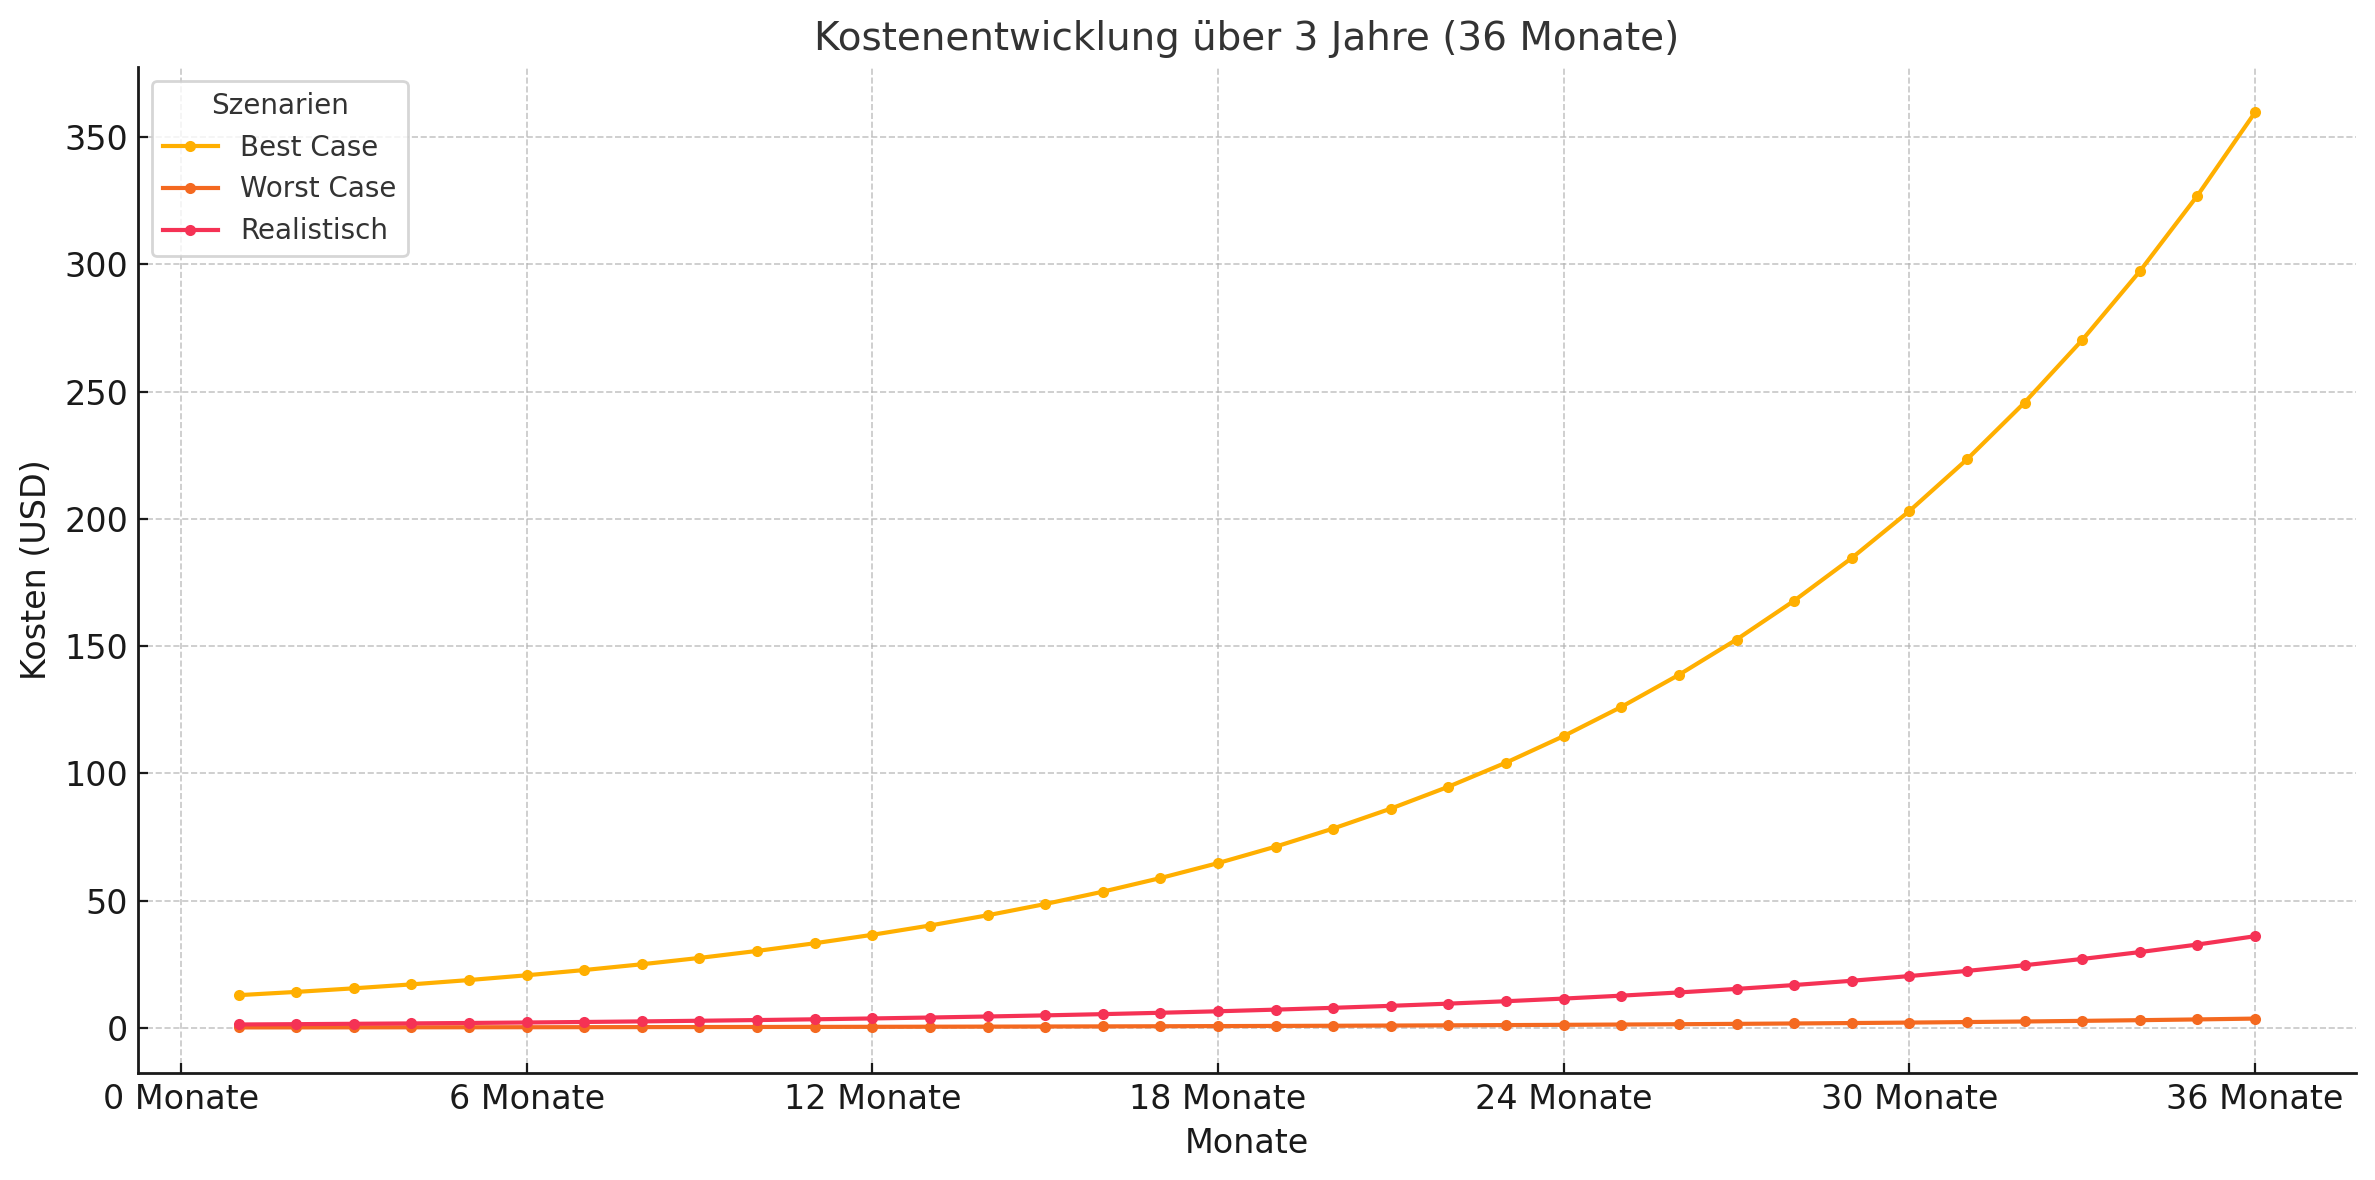
\includegraphics[width=\textwidth, height=\textheight, keepaspectratio]{abbildungen/KostenSpeicher}
    \caption{Kostenentwicklung für die Speicherung von Bildern über 3 Jahre}
    \label{fig:KostenentwicklungSpeicher}
    \raggedright Quelle: Eigene Darstellung
\end{figure}

\textbf{Generierung und Speicherung von Texten}\newline
Die Textgenerierung wird mit dem Text-to-Text-Modell Mistral-7B-Instruct durchgeführt, welches ebenfalls auf der Google Cloud Plattform als Endpunkt bereitgestellt wird.
Dabei wird die gleiche Konfiguration wie beim Bildmodell verwendet, entsprechend Region Belgien und n1-standard-4 als Maschine.
Die anfallenden Maschinenstunden werden jedoch geringer angenommen, da die Inferenzzeit pro Anfrage im Testbetrieb bei ca. 100 ms lag.

Daraus ergeben sich folgende Kostenstrukturen:
\begin{itemize}
    \item Best Case: 5000 User * 10 Anfragen * 0,1 s * 0,24 USD = 120 USD
    \item Worst Case: 50 User * 10 Anfragen * 0,1 s * 0,24 USD = 1,2 USD
    \item Realistisches Szenario: 500 User * 10 Anfragen * 0,1 s * 0,24 USD = 12 USD
\end{itemize}

Zum Speichern der generierten Texte wird der Data Store verwendet.
Dieser wird in der Region Belgien gehostet und wird nach Lese- und Schreibvorgängen, sowie den gespeicherten Daten berechnet.

\begin{figure}[htbp]
    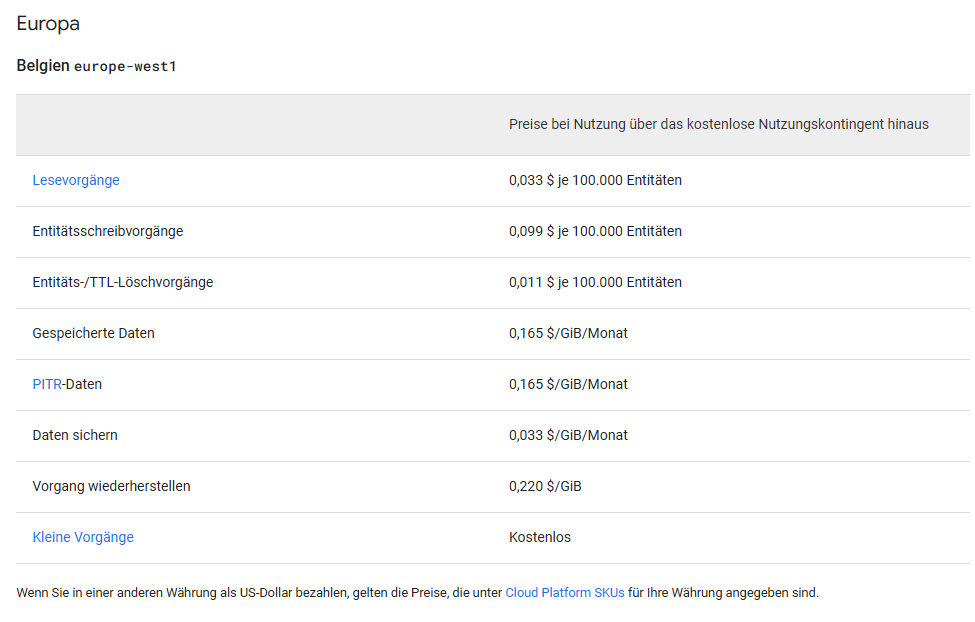
\includegraphics[width=\textwidth, height=\textheight, keepaspectratio]{abbildungen/kostendatastore}
    \caption{Kostenstruktur Data Store}
    \label{fig:KostenDataStore}
    \raggedright Quelle:\cite{GoogleDatastorePricing2025}
\end{figure}


Dabei wird nur die Nutzung abgerechnet, welche die Freikontingente überschreitet.
Dies wird einzig im Best Case Szenario eintreten, da die Freikontingente für die anderen Szenarien ausreichen.
Selbst im Best Case Szenario ist anzunehmen, dass einzig das Freikontingent für Schreibvorgänge minimal überschritten wird.
Dieses wird pro 100.000 Schreibvorgängen mit 0,099 USD berechnet, weshalb diese Kosten vernachlässigbar sind.

Für den Speicherbedarf ist zu beachten, dass der Text bei einem Social-Media-Post bei durchschnittlich 200 Zeichen liegen kann.

\begin{itemize}
    \item \textbf{Best Case}
    \begin{itemize}
        \item \textbf{2025:} \(5000 \, \text{User} \times 24 \, \text{kB} = 117,19 \, \text{MB}\)
        \item \textbf{2026:} \(117,19 \, \text{MB} + (6000 \, \text{User} \times 24 \, \text{kB}) = 263,06 \, \text{MB}\)
        \item \textbf{2027:} \(263,06 \, \text{MB} + (7200 \, \text{User} \times 24 \, \text{kB}) = 440,25 \, \text{MB}\)
    \end{itemize}

    \item \textbf{Realistic Case}
    \begin{itemize}
        \item \textbf{2025:} \(500 \, \text{User} \times 24 \, \text{kB} = 11,72 \, \text{MB}\)
        \item \textbf{2026:} \(11,72 \, \text{MB} + (600 \, \text{User} \times 24 \, \text{kB}) = 26,31 \, \text{MB}\)
        \item \textbf{2027:} \(26,31 \, \text{MB} + (720 \, \text{User} \times 24 \, \text{kB}) = 44,03 \, \text{MB}\)
    \end{itemize}

    \item \textbf{Worst Case}
    \begin{itemize}
        \item \textbf{2025:} \(50 \, \text{User} \times 24 \, \text{kB} = 1,17 \, \text{MB}\)
        \item \textbf{2026:} \(1,17 \, \text{MB} + (60 \, \text{User} \times 24 \, \text{kB}) = 2,63 \, \text{MB}\)
        \item \textbf{2027:} \(2,63 \, \text{MB} + (72 \, \text{User} \times 24 \, \text{kB}) = 4,40 \, \text{MB}\)
    \end{itemize}
\end{itemize}

Daraus ergeben sich folgende Kosten in den kommenden drei Jahren:
\begin{figure}[htbp]
    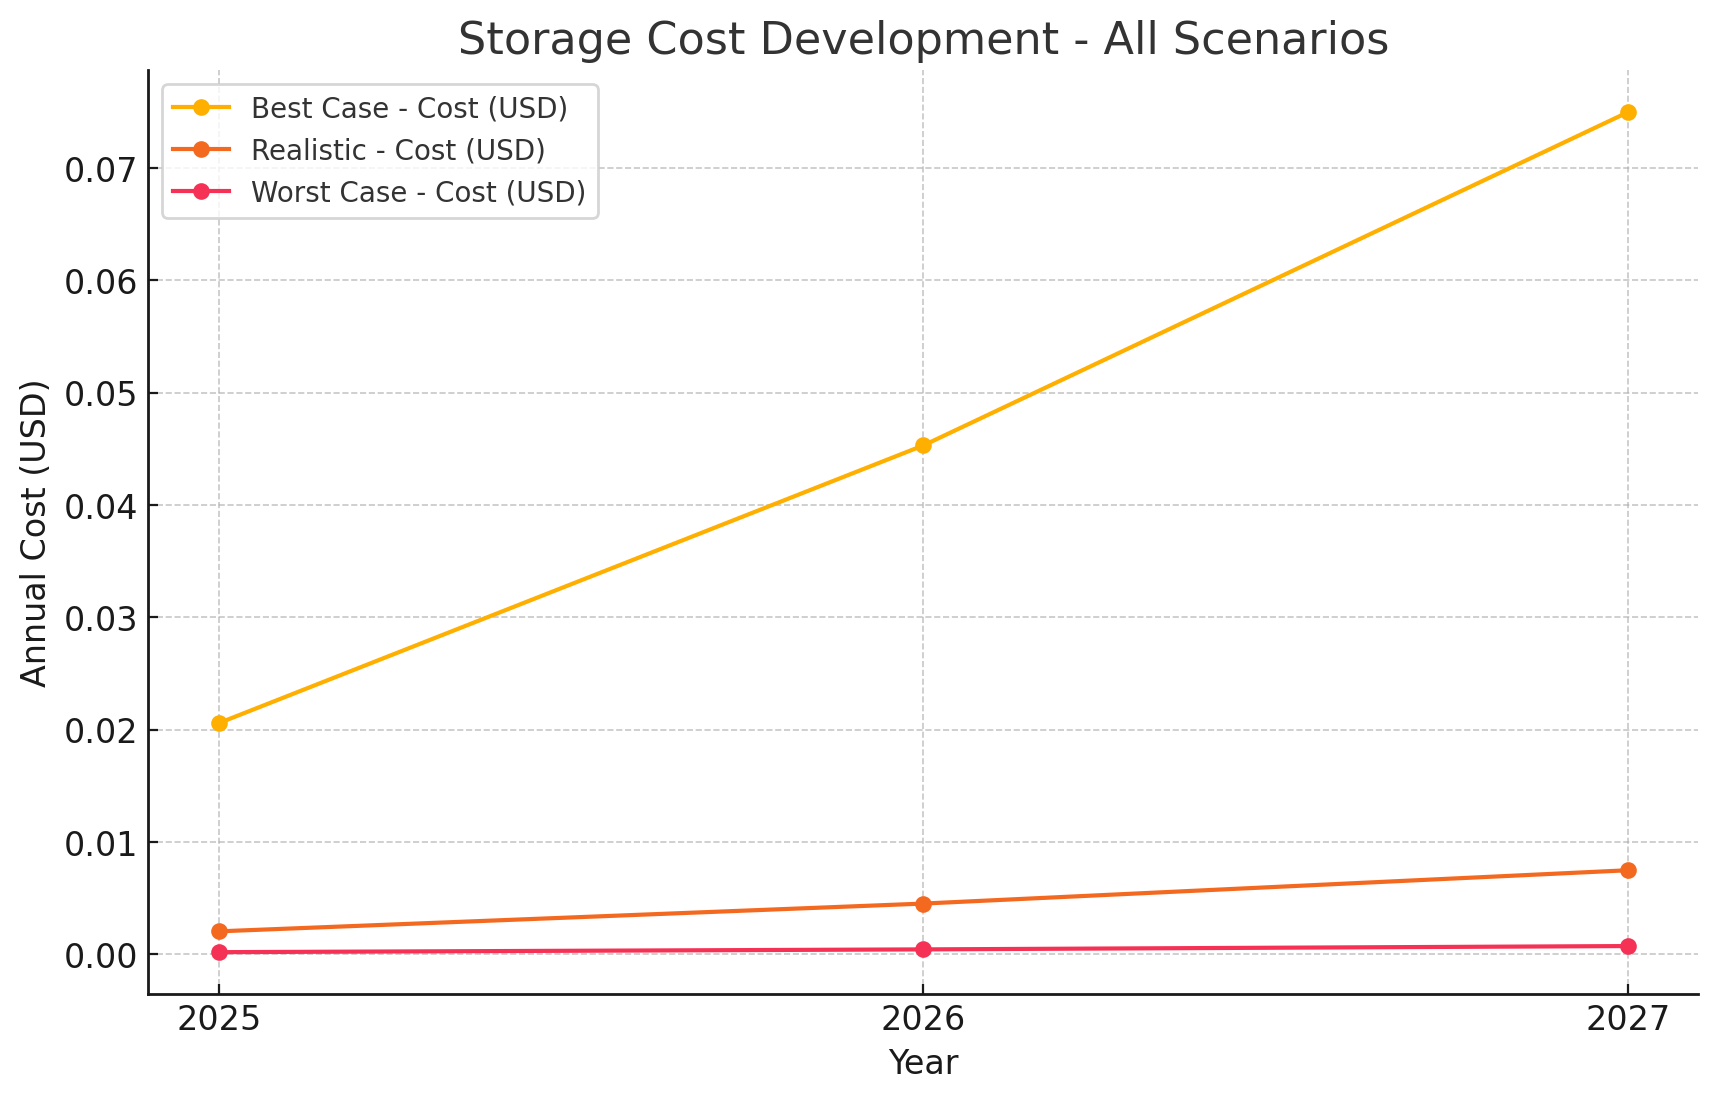
\includegraphics[width=\textwidth, height=\textheight, keepaspectratio]{abbildungen/Kosten_Speicher_Text}
    \caption{Entwicklung der Speicherkosten für Texte über 3 Jahre}
    \label{fig:KostenentwicklungSpeicherText}
    \raggedright Quelle: Eigene Darstellung
\end{figure}

Dabei ist über die Jahre bereits ein realisiertes Wachstum betrachtet, welches sich in den Kosten widerspiegelt.
Dennoch sind selbst im Best Case Szenario die Kosten für den Speicherplatz im Data Store vernachlässigbar.

\textbf{Plattform}\newline
Die Plattform setzt sich aus folgenden Komponenten zusammen:
\begin{itemize}
    \item Google Kubernetes Engine Cluster
    \item Google Cloud CDN
    \item Enabler Services (Monitoring, Logging, IAM, Secret Manager)
\end{itemize}

In der Ramp-Up-Phase wird die Plattform mit einer minimalen Konfiguration betrieben.
Die Funktion der Enterprise-Version sind für die ersten drei Jahre nicht notwendig und werden daher nicht betrachtet.
Dementsprechend wird die Standardversion von der Google Kubernetes Engine verwendet, welche 0,10 USD pro Stunde kostet.\footcite{GoogleKubernetesEnginePricing2025}
Bei einem Betrieb von 24 Stunden am Tag ergeben sich folgende Kosten für die drei Jahre:

0,10 USD * 24 h * 365 Tage * 3 Jahre = 2628 USD

Zusätzlich sind die Kosten für die Enabler Services zu betrachten.

Für das Monitoring werden Kosten erhoben, basierend auf dem benötigen Speicher, sowie dem Aufrufen der erhobenen Daten.

\begin{itemize}
    \item 0,2580 USD/MiB: erste 150–100.000 USD/MiB
    \item 0,1510 USD/MiB: nächste 100.000–250.000 USD/MiB
    \item 0,0610 USD/MiB: >250.000 USD/MiB
\end{itemize}

Die Aufrufe werden mit 0,01 USD/1.000API-Leseaufruf abgerechnet, wobei API-Schreibaufrufe kostenlos sind.

Die Plattform setzt sich aus drei Kubernetes Deployments zusammen.
Diese werden mit jeweils 2 Pods betrieben, um eine hohe Verfügbarkeit zu gewährleisten.
Daraus lässt sich ein grober Bedarf an Speicher von 1 GB ableiten, welcher für die ersten drei Jahre ausreicht.
Dieser lässt sich mit unterschiedlichen Speicherzeitrahmen reduzieren.
Wenn die Monitoring-Daten für 30 Tage gespeichert werden, ergibt sich ein Speicherbedarf von ca. 84,11 MiB.
Wird dieser auf die Kostenstruktur angewendet, ergeben sich näherungsweise folgende Kosten für die drei Jahre:

0,2580 USD/MiB * 84,11 MiB * 365 Tage * 3 Jahre = 7,5 USD

Zur Vereinfachung der Berechnung werden ähnliche Kosten für das Logging angenommen.

Für die Nutzung des \ac{IAM} Services fallen keine Kosten an.\footcite{GoogleIAMPricing2025}
Für den Secret Manager ist in der Standardversion eine Nutzung von 100 Secrets kostenlos, weshalb auch hier keine Kosten anfallen.\footcite{GoogleSecretManagerPricing2025}

\textbf{Personalkosten}\newline
Für die Weiterentwicklung des Produktes werden zwei Entwickler benötigt.
Für den Betrieb des Produktes, im Sinne von Support, wird ein Service-Desk Mitarbeiter benötigt.
Die Kosten für einen Entwickler belaufen sich auf 100€ die Stunde und für einen Service-Desk Mitarbeiter auf 35€ die Stunde.


\textbf{Entwicklungskosten}\newline
Zur Entwicklung der Plattform sind nach Abschluss dieser Arbeit noch folgende Arbeiten notwendig, um ein produktiven Betrieb zu gewährleisten:
\begin{itemize}
    \item Entwicklung und Anpassung der Frontend-Applikation
    \item Anpassen der Kubernetes Deployments
    \item Einrichten der Enabler Services
    \item Einrichten des Data Store + Google Cloud Storage
    \item Einrichten des CDN
    \item Ende-zu-Ende-Tests
    \item Aufbau Support- und Wartungsstruktur
\end{itemize}

Zur Berechnung der Entwicklungskosten sind folgende Annahmen zu treffen:
\begin{itemize}
    \item Stundensatz Entwickler: 100 Euro
    \item Entwicklungsteam: 5 Entwickler
\end{itemize}

Zur Erfassung der Aufwände werden grobe \ac{FTE} angenommen, welche die Entwicklungskosten für die ersten drei Jahre darstellen.
Damit ergeben sich folgende Kosten:
\begin{itemize}
    \item Entwicklung und Anpassung der Frontend-Applikation - 5 \ac{FTE}
    \item Anpassen der Kubernetes Deployments - 2 \ac{FTE}
    \item Einrichten der Enabler Services - 2 \ac{FTE}
    \item Einrichten des Data Store + Google Cloud Storage - 1 \ac{FTE}
    \item Einrichten des CDN - 1 \ac{FTE}
    \item Ende-zu-Ende-Tests - 5 \ac{FTE}
    \item Aufbau Support- und Wartungsstruktur 3 \ac{FTE}
\end{itemize}

Daraus ergeben sich grob folgende Personalkosten:
19 \ac{FTE} * 8 Stunden * 100 Euro = 15.200 Euro

Zusätzlich sind die Kosten für die Entwicklungsumgebung zu betrachten.
Diese teilt sich in das Bereitstellen des notwendigen Toolings, sowie einer Testumgebung auf.
Da die restaufwände lediglich ein kleines Team bestehend aus 5 Entwicklern benötigen, fallen keine nennenswerten Kosten für die Entwicklungsumgebung an.
Einzig relevant sind die Lizenzkosten für die benötigten Entwicklungsumgebungen, welche mit 100 Euro pro Entwickler pro Monat angenommen werden.

Um die finalen Aufwände leisten zu können wird ein Zeitraum von 2 Monaten angenommen, in welchem die Entwicklung abgeschlossen wird.
Daraus ergeben sich folgende Kosten:
5 Entwickler * 100 Euro * 2 Monate = 1000 Euro

Zusammenfassend ergeben sich folgende Entwicklungskosten:
15.200 Euro + 1000 Euro = 16.200 Euro

%(Pricing Modell Auswahl)

Das Freemium-Bezahlmodell, bei welchem Nutzer der Applikation erst nach einer gewissen Anzahl von Social-Media-Posts monatlich bezahlen müssen, bietet eine Möglichkeit die Kosten für den Betrieb und die Entwicklung der Anwendung zu amortisieren.
Die Kosten für die Premiumvariante sind so zu wählen, dass sie die Betriebskosten tragen können und eine Gewinnmarge erwirtschaftet werden kann.
Gleichzeitig muss bei der Preisgestaltung berücksichtigt werden, dass man diese nicht zu hoch ansetzt und diese in Relation zu den Wettbewerbern steht.
Kilian, die Applikation, welche auf Contentgenerierung innerhalb der Gastronomie- und Hotelbranche spezialisiert ist, nimmt mit der Premiumvariante mindestens 23€ pro Monat ein.
Die Lösung des Unternehmens MARA nimmt für seine GenAI-basierende Lösung in der Premiumvariante je Zugang 99€ pro Monat ein.
Jasper stellt sich mit zwei verschieden Varianten auf, der Startervariante mit 30€ pro Monat und der Boss-Mode-Variante mit 60€ pro Monat.
Unter der Betrachtung der Konkurrenten wird ein Einstandspreis von 20€ pro Monat bestimmt, damit diese Lösung die günstigste am Markt ist und viele Kunden anlocken kann.
Unter der Betrachtung der drei skizzierten Szenarien (50, 500, 5000 Nutzer) könnten folgende Ertragskalkulationen eintreffen:

50 Nutzer + 20€ pro Monat = 1.000€ pro Monat
500 Nutzer + 20€ pro Monat = 10.000€ pro Monat
5000 Nutzer +20€ pro Monat = 100.000€ pro Monat

%(Sonstige Einnahmen)

Ein weiterer Aspekt in der Einnahme spiegeln die erhobenen Daten, wie die Prompts und generierten Social-Media-Posts, wider.
Diese können ein Einblick in die Gastronomie vermitteln und wichtige Rückschlüsse für die Entwicklung von Produkten suggerieren.
Dementsprechend könnten diese Daten von hohem Interesse für Unternehmen sein, die ggf. selber in die Gastronomie einsteigen wollen oder Produkte für die Gastronomie entwickeln wollen.
Der Wert dieser Daten bestimmt sich im Volumen und Qualität der abgegebenen Daten.
Da sich die Applikation in den Anfängen befindet, wird der Verkauf von Nutzerdaten erstmal nicht betrachtet.

%(Break Even Analyse)
Eine Break-Even-Analyse erlaubt die Betrachtung, ab welchem Zeitpunkt sich der Betrieb der Lösung wirtschaftlich rentiert.
Die Betrachtung erfolgt auf monatlicher Basis.
Das impliziert, dass sämtliche Kosten auf einen monatlichen Faktor runtergebrochen werden, ebenso, wie die Erträge.
Daraus ergibt sich, dass die Anwendung ca. 3760 zahlende Nutzer benötigt, um den Break-Even-Point zu erreichen.

\begin{figure}[htbp]
    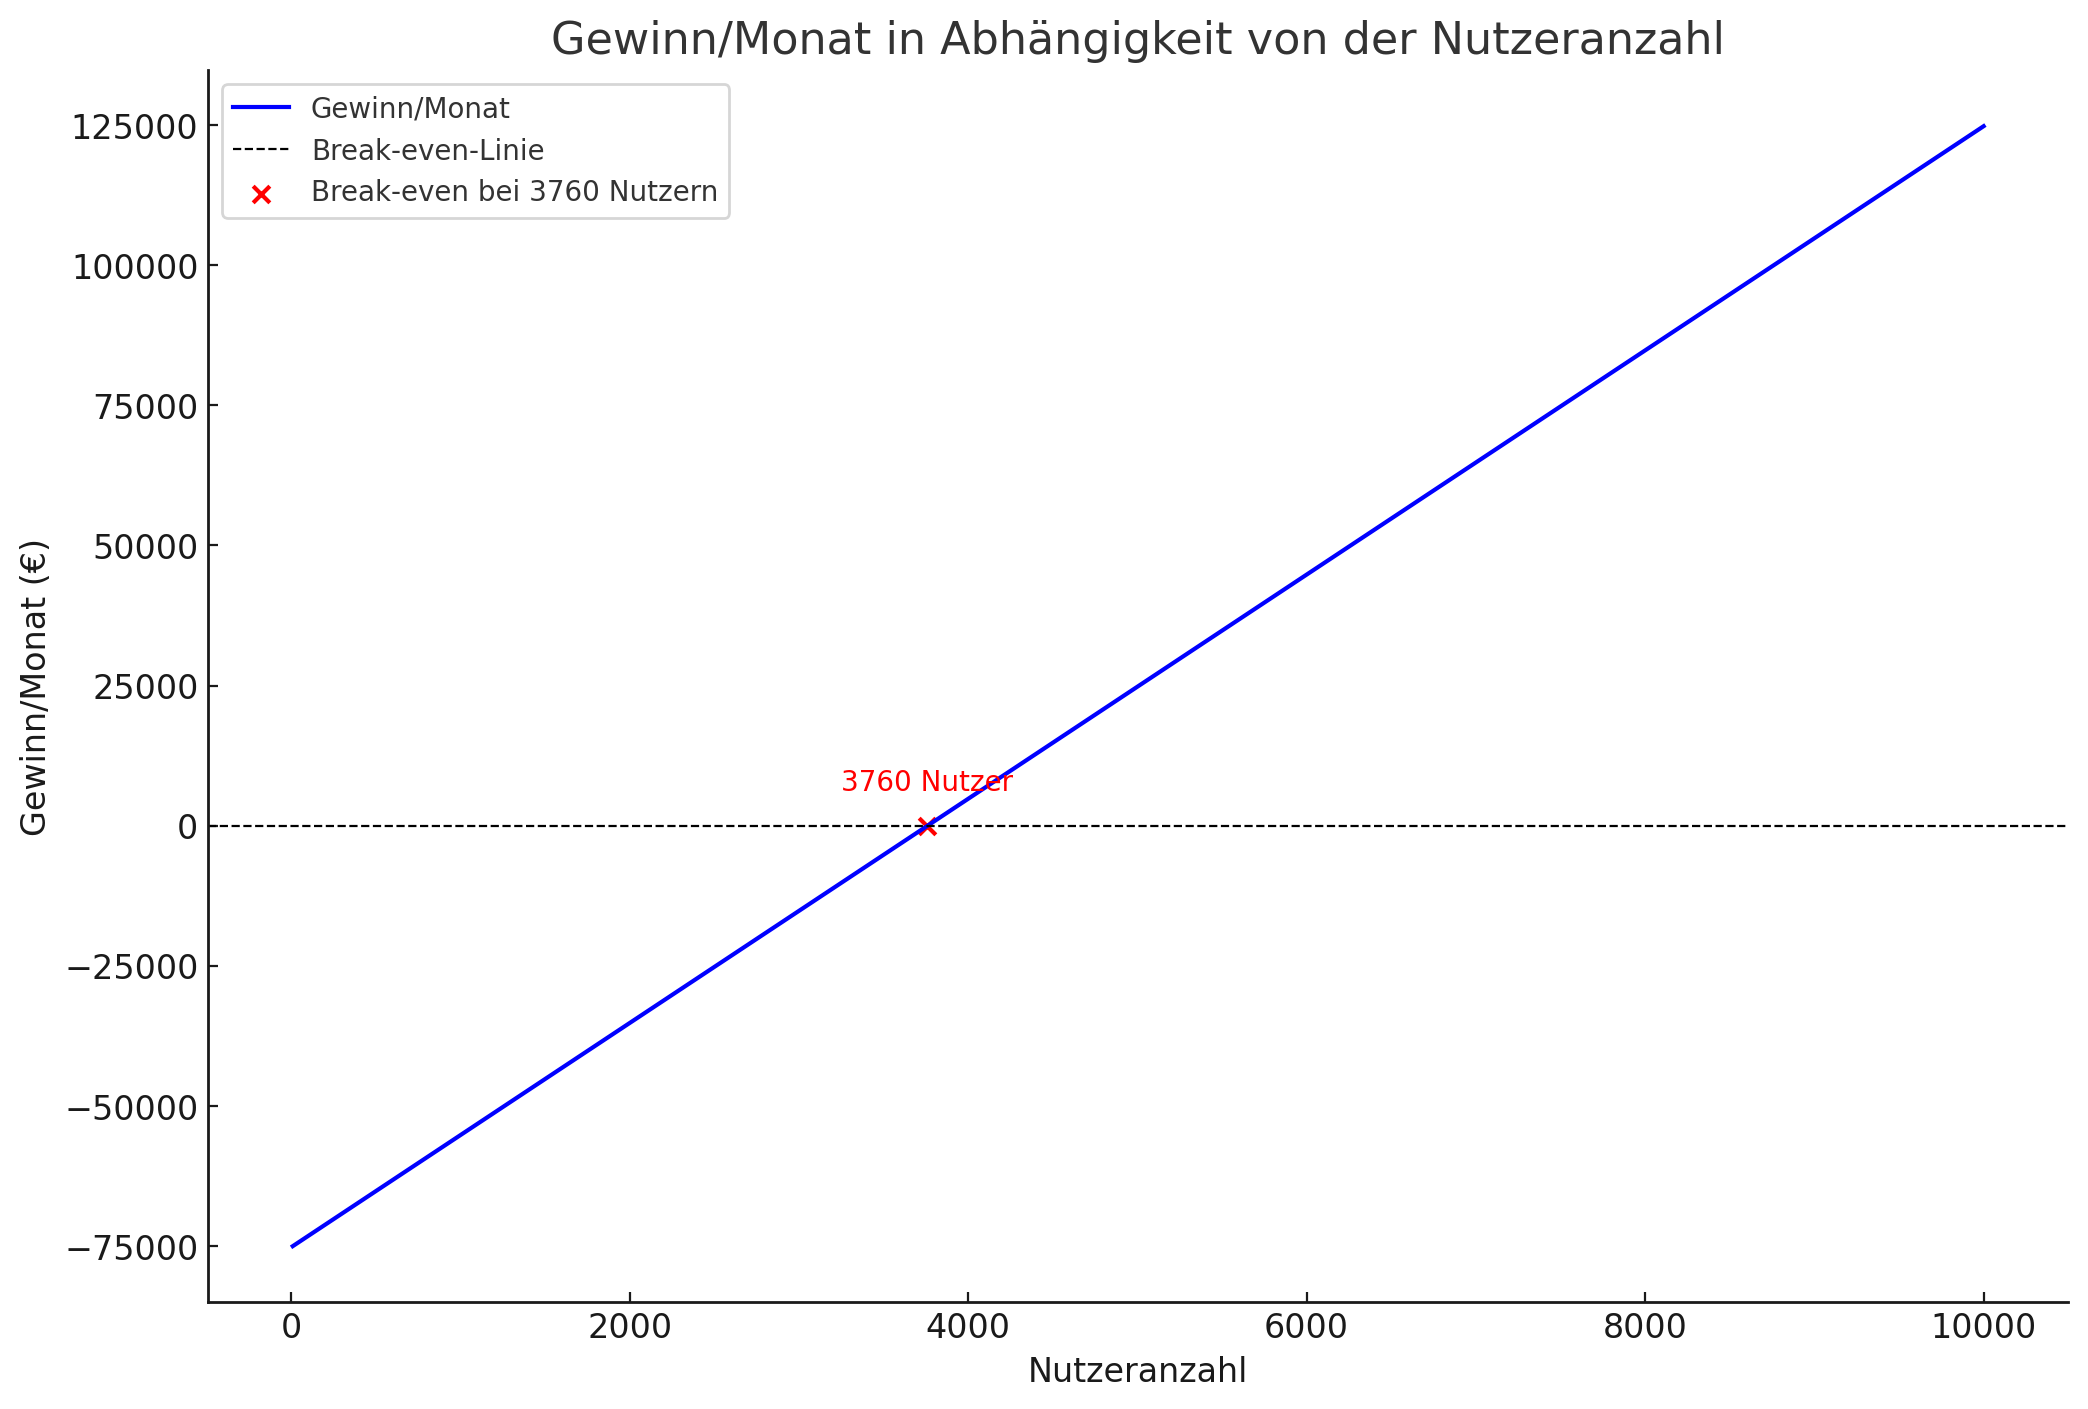
\includegraphics[width=\textwidth, height=\textheight, keepaspectratio]{abbildungen/Break_Even}
    \caption{Break Even Analyse}
    \label{fig:BreakEven}
    \raggedright Quelle: Eigene Darstellung
\end{figure}
\newpage
\section{Schlussbetrachtung}

\subsection{Zusammenfassung der Ergebnisse}

Analyse Forschungsstand

Im Rahmen dieser Projektarbeit wurde auf Basis verschiedener analytischer und konzeptioneller Methoden ein Konzept für eine KI-gestützte Social Media Marketing Plattform entwickelt.
Zur Fundierung des erarbeiteten Konzepts wurde eine weitreichende Analyse der Kundenbedürfnisse und der Wettbewerbslage durchgeführt.
Die daraus abgeleiteten Erkenntnisse wurden durch eine SWOT-Analyse ergänzt, um eine geschärfte Sicht auf die Stärken und Schwächen, sowie mögliche Chancen und Risiken des angestrebten Produkts zu erhalten.
Anknüpfend an die vorangegangenen Analysen wurde, innerhalb eines ausführlichen Vergleichs verschiedener Plattform, Instagram als geeignete Social Media Plattform ausgewählt.

Zur finanziellen Perspektive des Projekts wurde eine Strategie zur Monetarisierung der Plattform entwickelt, welche zentral auf einem Freemium-Modell basiert.
Dabei wurde zudem betrachtet, neben der direkten Monetarisierung durch den Umsatz der Abonnements, weitere indirekte Einnahmequellen zu erschließen, die sich beispielsweise durch das Sammeln von Daten über das Nutzerverhalten ergeben.

Um die technische Konzeptionierung vollständig zu ermöglichen, wurden die wichtigsten Eigenschaften der Social Media Posts untersucht, basierend auf verschiedenen vorangegangen Studien.
Die identifizierten Eigenschaften stellen den Kern der zu generierenden Inhalte dar.

Zur Erarbeitung des technischen Konzepts wurde eine umfassende Evaluierung der einzusetzenden Technologien durchgeführt.
Die Evaluierung gliedert sich in die Untersuchung der einzusetzenden Large Language Modelle zur Generierung von Texten und Bildern, sowie benötigte Komponenten der Webanwendung, inklusive deren Betrieb.
Dies wurde im Hinblick auf den Einsatz der Google Cloud Platform durchgeführt, welche verschiedene Dienste beinhaltet, die den Betrieb der Plattform ermöglichen.

Die Evaluation der Large Language Modelle wurde durch einen praktischen Vergleich verschiedener Modelle durchgeführt.
Bei der Evaluation der einzusetzenden Technologien für die Webanwendung wurde die Paprika-Methode angewendet, um die verschiedenen Komponenten zu realisieren.
Durch dieses Vorgehen konnte insgesamt ein Text-Generierungsmodell, ein Bild-Generierungsmodell, sowie die Technologien für Frontend, Backend und Datenbank ausgewählt werden.

Im nächsten Schritt wurde ein Erstentwurf der App entwickelt, welcher sowohl den Aufbau der Plattform, als auch die visuelle Gestaltung der Plattform umfasst.
Der Entwurf beinhaltet dazu eine UX Guideline, welche eine einheitliche Gestaltung der Plattform sicherstellt.
Diese UX Guideline wurde in ersten Entwürfen der Landing Page, des Dialogs, des Post Editors und der Kalenderansicht umgesetzt.

Zur Darstellung des Aufbaus der Plattform wurde ein Architekturmodell entwickelt, welches die verschiedenen Komponenten, als auch die Interaktionen zwischen diesen, darstellt.
Dieses besteht zum einen aus den benötigten Services der Google Cloud Platform, zum anderen aus den eigenen Microservices bzw. Frontends als Kubernetes Deployments.
Im Rahmen des Erstenwurfs wurde insbesondere der Aufbau der Kubernetes Deployments dargestellt.

Abschließend wurde, basierend auf dem Erstenwurf, eine Kostenschätzung durchgeführt, um die Rentabilität der geplanten Plattform zu bewerten.
Dabei wurden die entstehenden Kosten für verschiedene Szenarien betrachtet, wodurch eine Abschätzung des Break-Even-Points ermöglicht wurde.

\subsection{Handlungsempfehlungen}

Das entwickelte Konzept zeigt auf, das eine KI-gestützte Social Media Marketing Plattform eine vielversprechende Möglichkeit darstellt, die aktuellen Bedürfnisse von Unternehmen im Gastronomiebereich, im Hinblick auf die Erstellung von Social Media Inhalten, zu adressieren.
Abgleitet aus den Ergebnissen dieser Arbeit ist es schlussfolgernd empfehlenswert, eine solche Plattform zu entwickeln.
Dabei ist vornehmlich die Untersuchung der wichtigsten Eigenschaften von Social Media Posts sowie die daraus abgeleiteten Prompts für die Generierung von Inhalten von hoher Relevanz.
Diese stellen eine wissenschaftliche fundierte Strukturierung der Inhalte dar, welche eine hohe Qualität der generierten Inhalte ermöglicht.
Dabei ist zu erwarten, dass bei der Umsetzung in einem konkreten Anwendungsfall diese Erkenntnisse unverändert übernommen werden können.
Bei der Erarbeitung des Prototypen und den initial durchgeführten Tests des Promptings, hat sich insbesondere gezeigt, dass die Qualität der generierten Inhalte gesteigert werden konnte, wenn die wichtigen Merkmale beachtet werden.
Als diese wurden unter anderem identifiziert, dass auf Kreativität, Einzigartigkeit, Zielgruppenorientierung, Konversionsorientierung, Bildbeiträge, persönliche und emotionale Ansprache sowie Story telling geachtet werden muss.

Bei den eingesetzten Technologien ist es empfehlenswert, diese auf Basis der gewonnenen Erkenntnisse auszuwählen.
Bei der Entwicklung des Prototypen wurden die Vorzüge der einzelnen Technologien deutlich, vornehmlich das moderne Frontend-Framework Vue.JS ermöglichte den Bau eines ersten Frontends.

Dennoch ermöglicht der Einsatz von Kubernetes als Betriebsplattform eine hohe Flexibilität, welche es ermöglicht, die Technologien im Laufe der Entwicklung anzupassen.
Dies kann beispielsweise notwendig sein, wenn das umsetzende Projektteam weitreichende Erfahrungen mit anderen verwandten Technologien hat.
Zudem ist das erstellte Architekturkonzept auf den Einsatz in der Google Cloud Platform ausgelegt, inklusive der zur Verfügung stehenden Dienste.
Bei der Umsetzung des Prototypen hat sich gezeigt, dass eine Integration innerhalb der, durch die Google Cloud Platform bereitgestellten, Dienste, eine schnelle Implementierung ermöglicht wird.
Dies wird durch die native Integration der verschiedenen Dienste weiter unterstützt.

Dadurch soll dieses Konzept möglichst weitreichend kompatibel mit den Anforderungen eines konkreten Anwendungsfalls sein.
Die im Konzept ausgewählten Dienste können dennoch durch äquivalente Dienste anderer Cloud-Anbieter ersetzt werden, falls dies im konkreten Anwendungsfall Vorteile bieten sollte.

Die im Rahmen des Erstenwurfs entwickelte UX Guideline, sowie die erstellen visuellen Entwürfe, vermitteln eine klare Vorstellung der geplanten Plattform.
Diese können in ein bestehendes UX Design System integriert werden, um die geplante Plattform in ein bestehendes Corporate Design zu integrieren.
Dabei ist es empfehlenswert, die in dieser Arbeit erstellten Konzepte in einem iterativen Prozess zu sichten und ggf. zu individualisieren, um die geplante Plattform in einem bestehenden Unternehmenskontext zu integrieren.
Die, in dieser Arbeit erarbeiteten visuellen Entwürfe, gliedern sich sowohl in einer konzeptionellen, als auch eine detailliertere Darstellung der Plattform als Figma Design.
Dadurch kann auf Basis der konzeptionellen Darstellung eine individuelle Anpassung an den konkreten Anwendungsfall erfolgen.

Die Kostenschätzung zeigt, dass sowohl der Use Case, als auch die geplante Architektur der Plattform, eine rentable Umsetzung ermöglichen.
Jedoch handelt es sich dabei um eine Abschätzung, welche auf verschiedenen Annahmen basiert, welche sich im konkreten Anwendungsfall noch ändern können.
Dabei ist insbesondere der geschätzte finanzielle Betriebsaufwand abhängig von individuellen Faktoren, wie beispielsweise spezielle Verträge mit Cloud-Anbietern oder Synergieeffekte durch andere Projekte.
Auch die Entwicklungskosten stellen lediglich einen Näherungswert dar, welcher im konkreten Anwendungsfall abweichen kann.
Zur Sicherstellung einer rentablen Umsetzung ist es daher empfehlenswert, die Kostenschätzung auf Basis des konkreten Anwendungsfalls zu überprüfen und gegebenenfalls anzupassen.

\subsection{Ausblick}
Die in diesem Konzept entwickelte KI-gestützte Social Media Marketing Plattform beschränkt sich auf den minimalen Funktionsumfang, um die Machbarkeit des Konzepts zu demonstrieren.
Dabei ist zentral hervorgegangen, dass durch den Einsatz von KI-Technologien eine hohe Qualität der generierten Inhalte erreicht werden kann.
Dabei wurde die Erhebung von Nutzerdaten, sowie das Auswerten dieser über eine entsprechende Business Intelligence Komponente, nicht weiter betrachtet, sondern lediglich als mögliche Erweiterung vorgesehen.
In einer weiterführenden Umsetzung erscheint es vielversprechend, diesen Aspekt weiter zu untersuchen, um dadurch die Nutzerdaten weiter zu monetarisieren.
Zudem liese sich die Plattform an weitere Social Media Plattformen anbinden, wodurch eine breitere Zielgruppe angesprochen werden kann.
Neben der Ausweitung der Plattform, kann auch eine Erweiterung der Zielbranche erfolgen, indem die Plattform an Bedürfnisse anderer Branchen angepasst wird, beispielsweise der Modebranche oder der Automobilbranche.
Dabei kann auf die zuvor durchgeführten Untersuchungen zurückgegriffen werden, welche die Eigenschaften der verschiedenen Plattformen untersucht haben.


%-----------------------------------
% Apendix / Anhang
%-----------------------------------
\newpage
\section*{\AppendixName} %Überschrift "Anhang", ohne Nummerierung
\addcontentsline{toc}{section}{\AppendixName} %Den Anhang ohne Nummer zum Inhaltsverzeichnis hinzufügen

\begin{appendices}
% Nachfolgende Änderungen erfolgten aufgrund von Issue 163
\makeatletter
\renewcommand\@seccntformat[1]{\csname the#1\endcsname:\quad}
\makeatother
\addtocontents{toc}{\protect\setcounter{tocdepth}{0}} %
	\renewcommand{\thesection}{\AppendixName\ \arabic{section}}
	\renewcommand\thesubsection{\AppendixName\ \arabic{section}.\arabic{subsection}}
	\section{Bilder Konzeptionierung}\label{sec:bilder-konzeptionierung}

\begin{figure}[htbp]
    \centering
    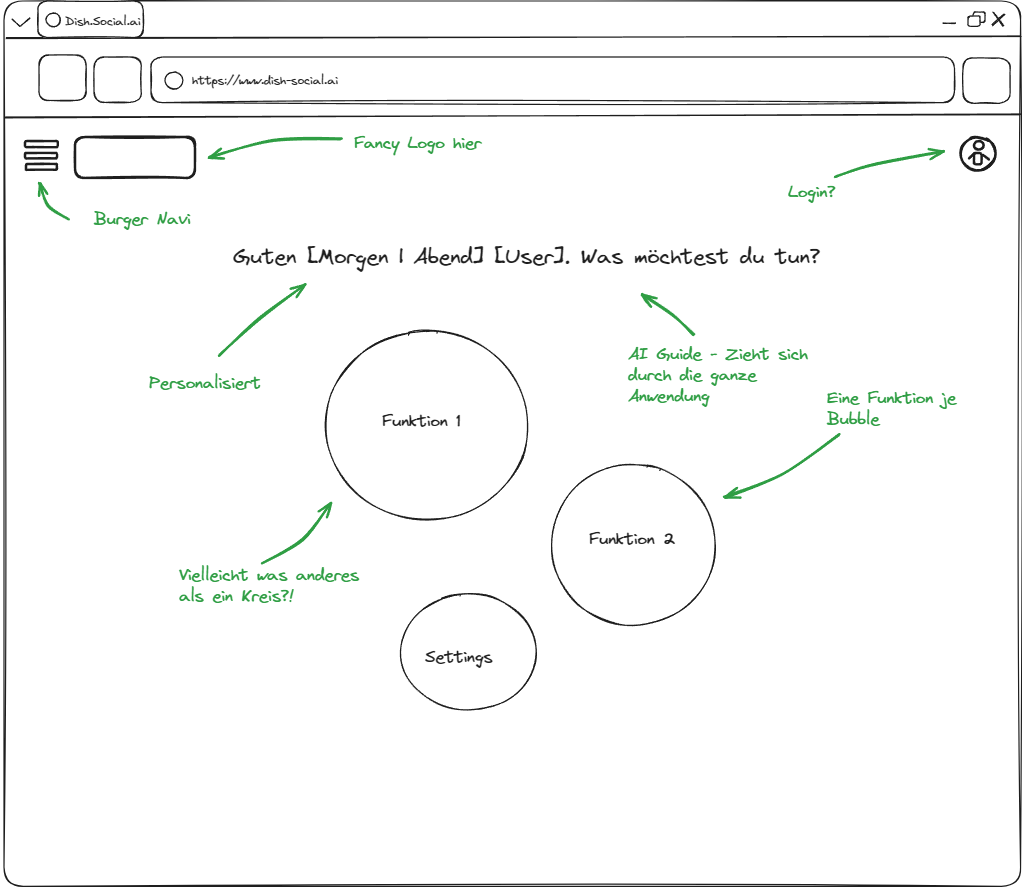
\includegraphics[width=\textwidth]{abbildungen/Konzept/Konzept Landing Page}
    \caption[]{Konzept Landing-Page Darstellung}
    \label{fig:landing-page-concept}
    \raggedright Quelle: Eigene Darstellung
\end{figure}
\newpage

\begin{figure}[htbp]
    \centering
    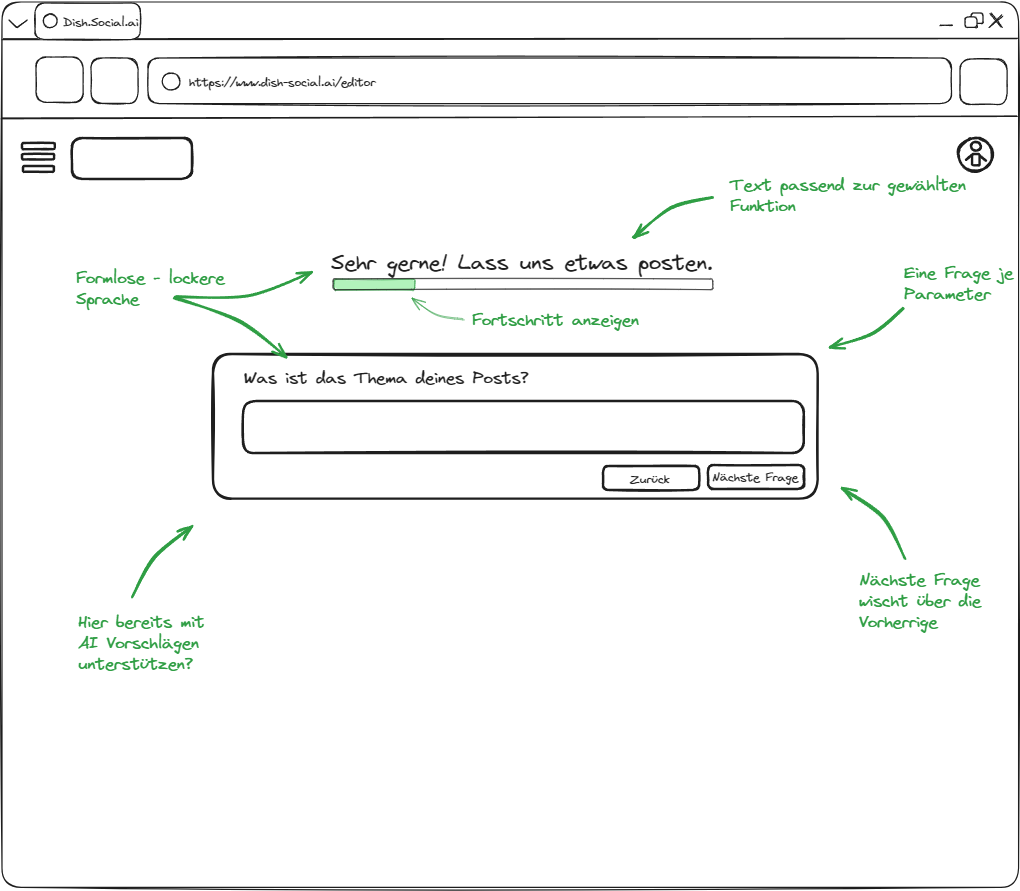
\includegraphics[width=\textwidth]{abbildungen/Konzept/Konzept Dialog}
    \caption[]{Konzept Dialog Darstellung}
    \label{fig:dialog-concept}
    \raggedright Quelle: Eigene Darstellung
\end{figure}
\newpage

\begin{figure}[htbp]
    \centering
    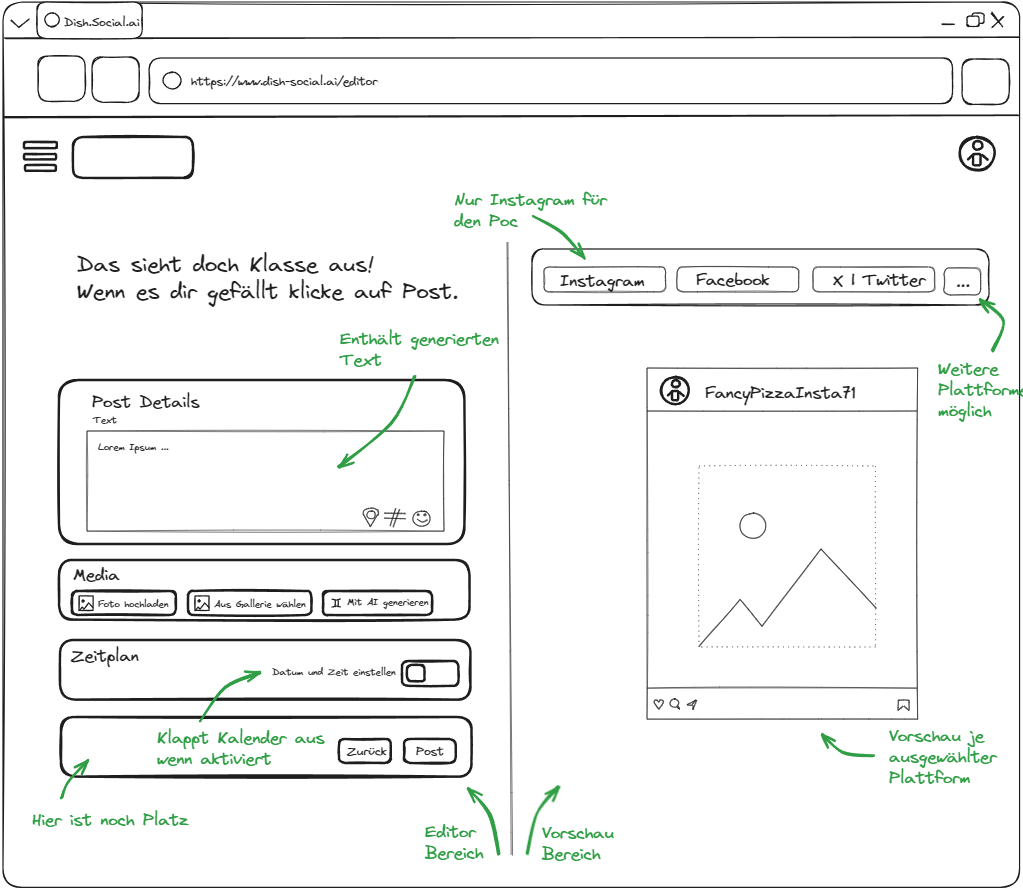
\includegraphics[width=\textwidth]{abbildungen/Konzept/Konzept Editor}
    \caption[]{Konzept Editor Darstellung}
    \label{fig:editor-concept}
    \raggedright Quelle: Eigene Darstellung
\end{figure}
\newpage

\begin{figure}[htbp]
    \centering
    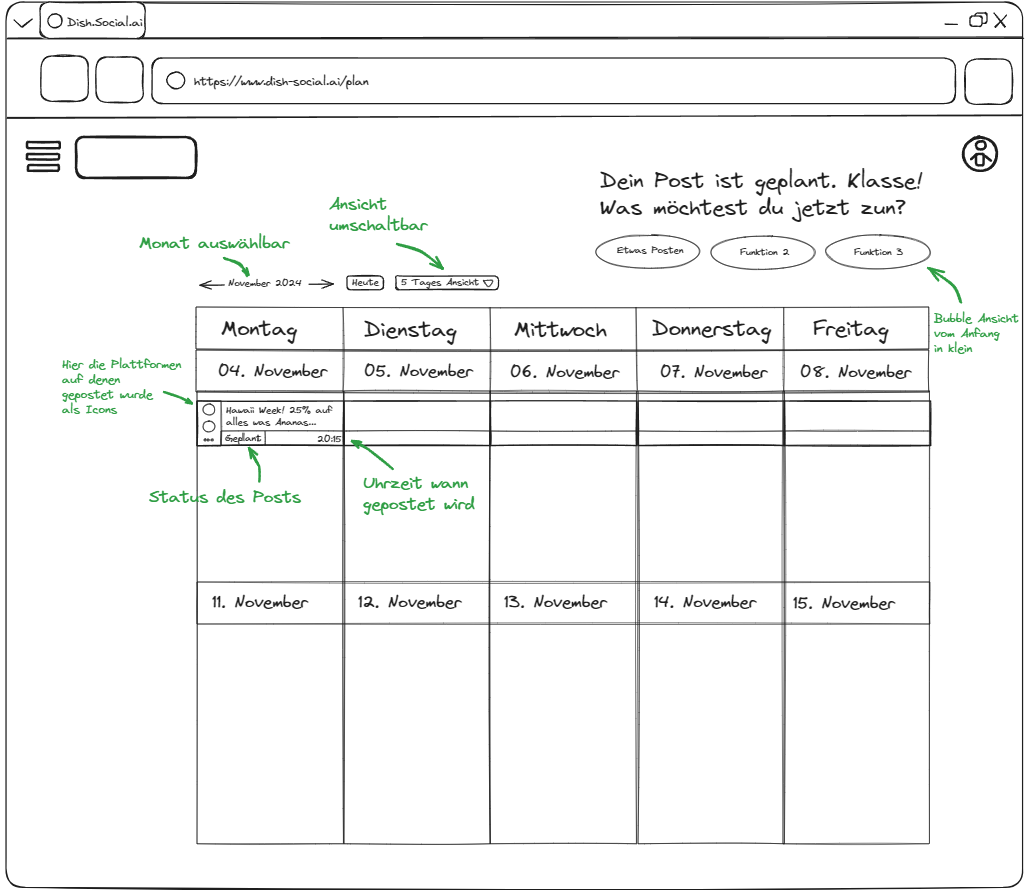
\includegraphics[width=\textwidth]{abbildungen/Konzept/Konzept Kalender}
    \caption[]{Konzept Kalender Darstellung}
    \label{fig:calendar-concept}
    \raggedright Quelle: Eigene Darstellung
\end{figure}
\newpage

\section{Bilder Figma Design}\label{sec:bilder-figma-design}
\begin{figure}[htbp]
    \centering
    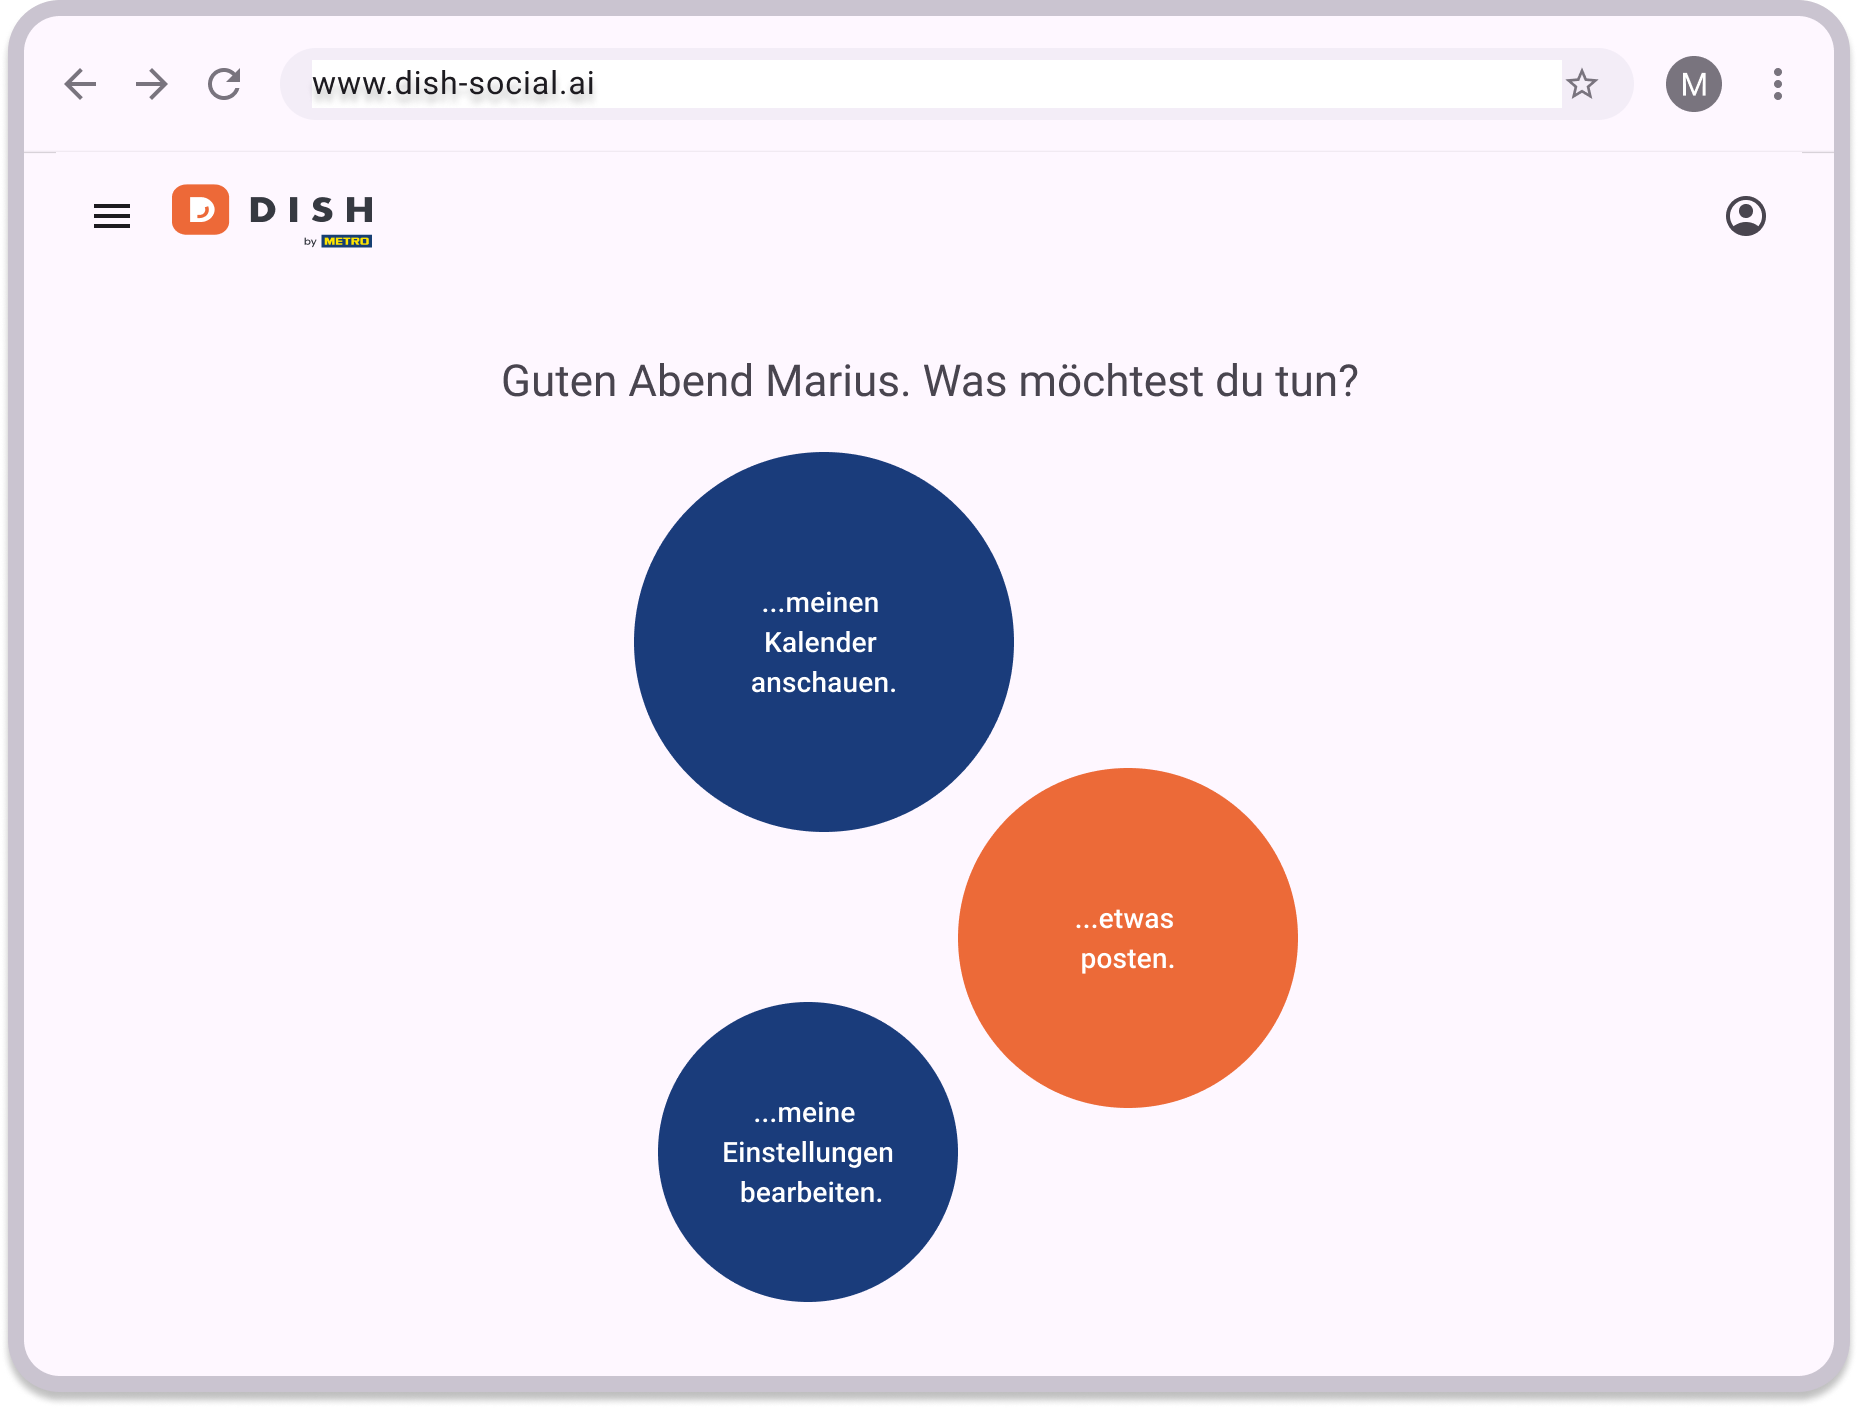
\includegraphics[width=\textwidth]{abbildungen/figma/Landing Page}
    \caption[]{Figma Design Landing-Page Darstellung}
    \label{fig:landing-page}
    \raggedright Quelle: Eigene Darstellung
\end{figure}
\newpage

\begin{figure}[htbp]
    \centering
    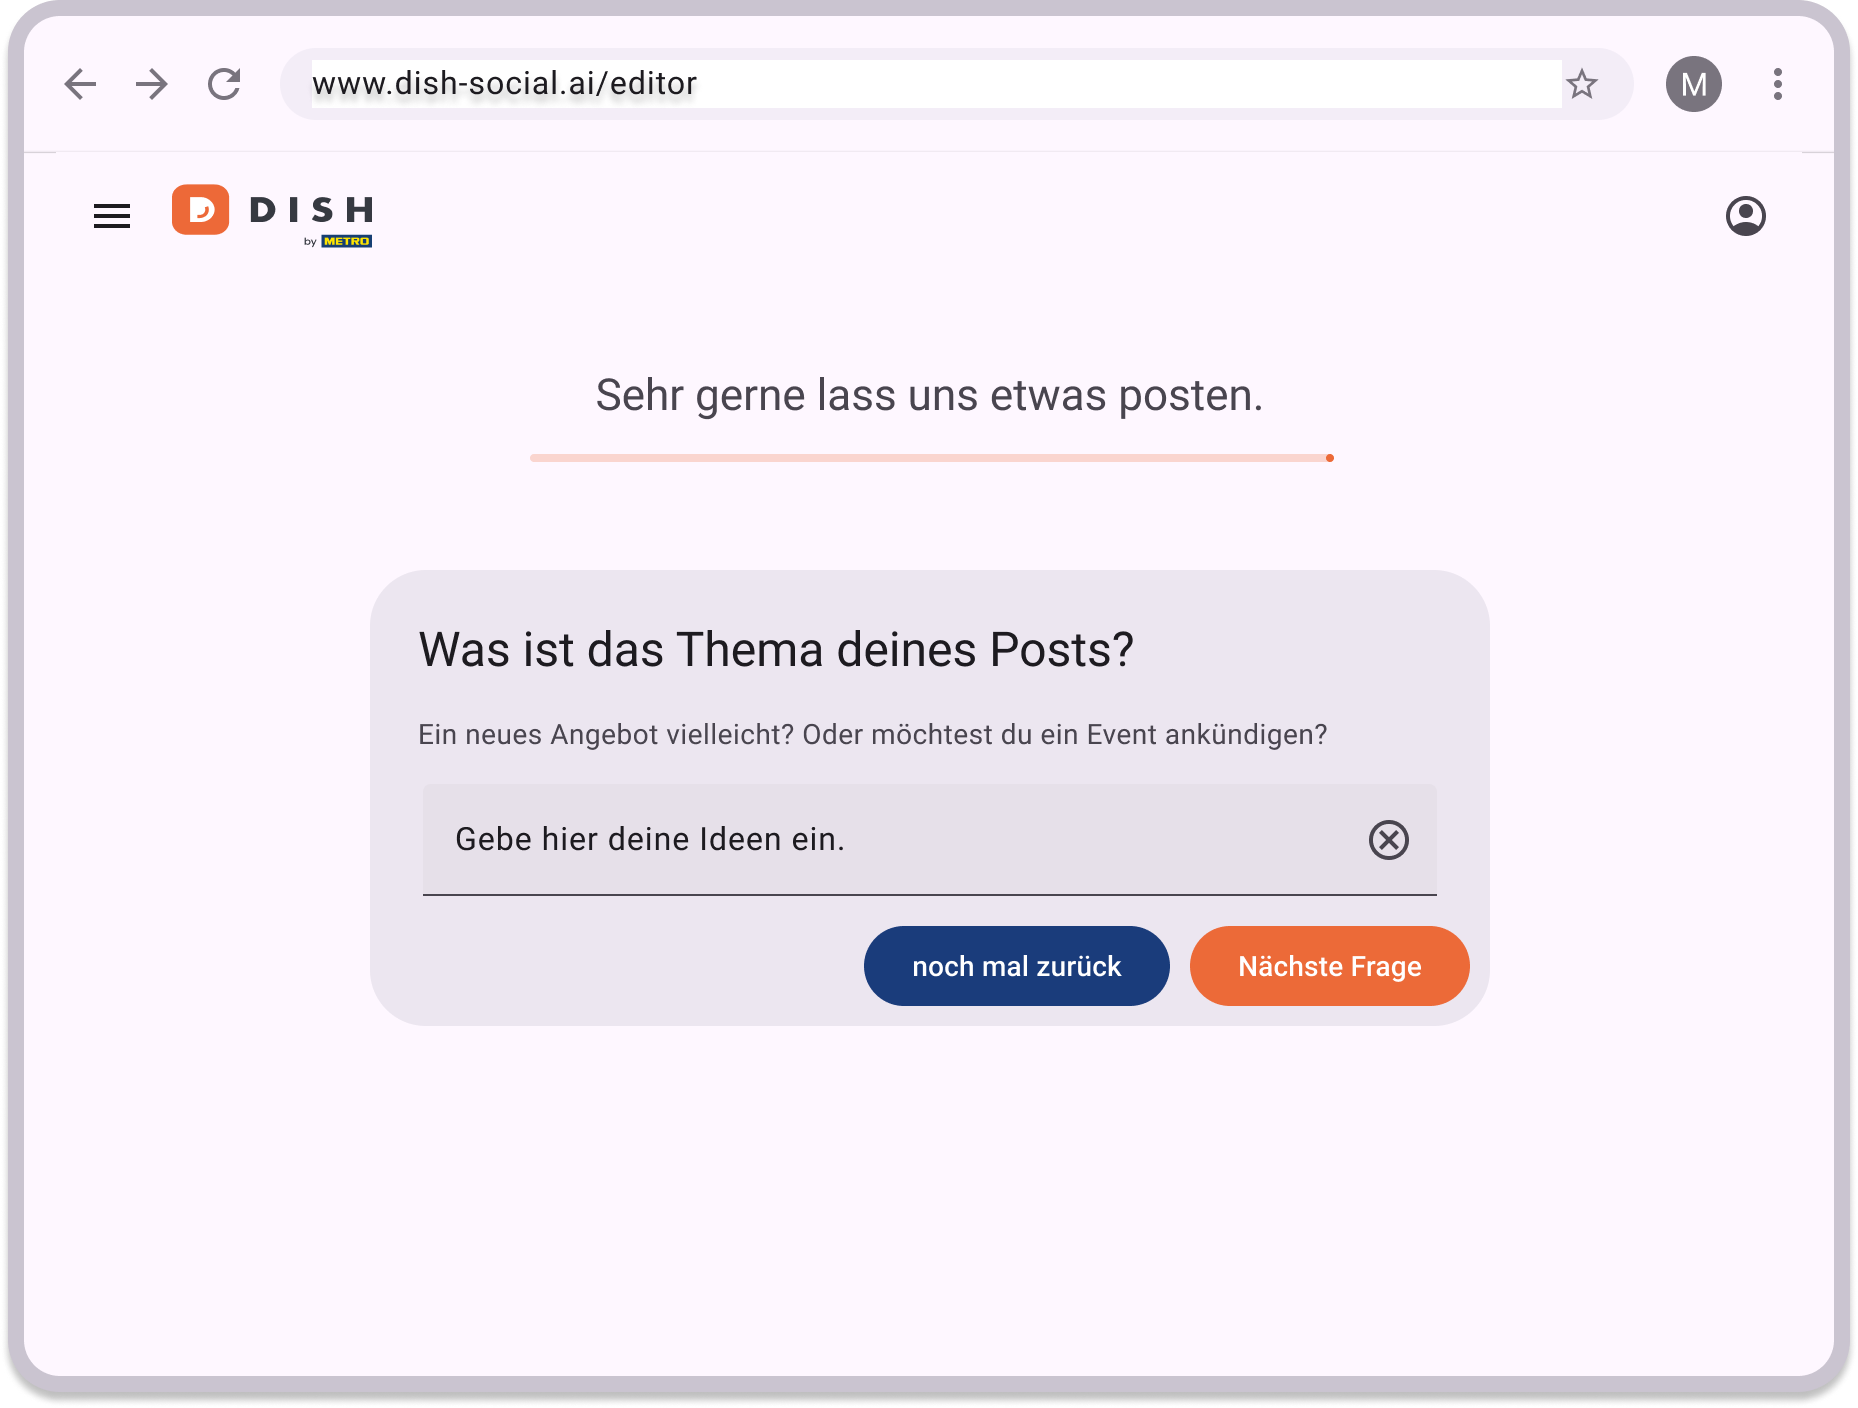
\includegraphics[width=\textwidth]{abbildungen/figma/Dialog}
    \caption[]{Figma Design Dialog Darstellung}
    \label{fig:dialog-page}
    \raggedright Quelle: Eigene Darstellung
\end{figure}
\newpage

\begin{figure}[htbp]
    \centering
    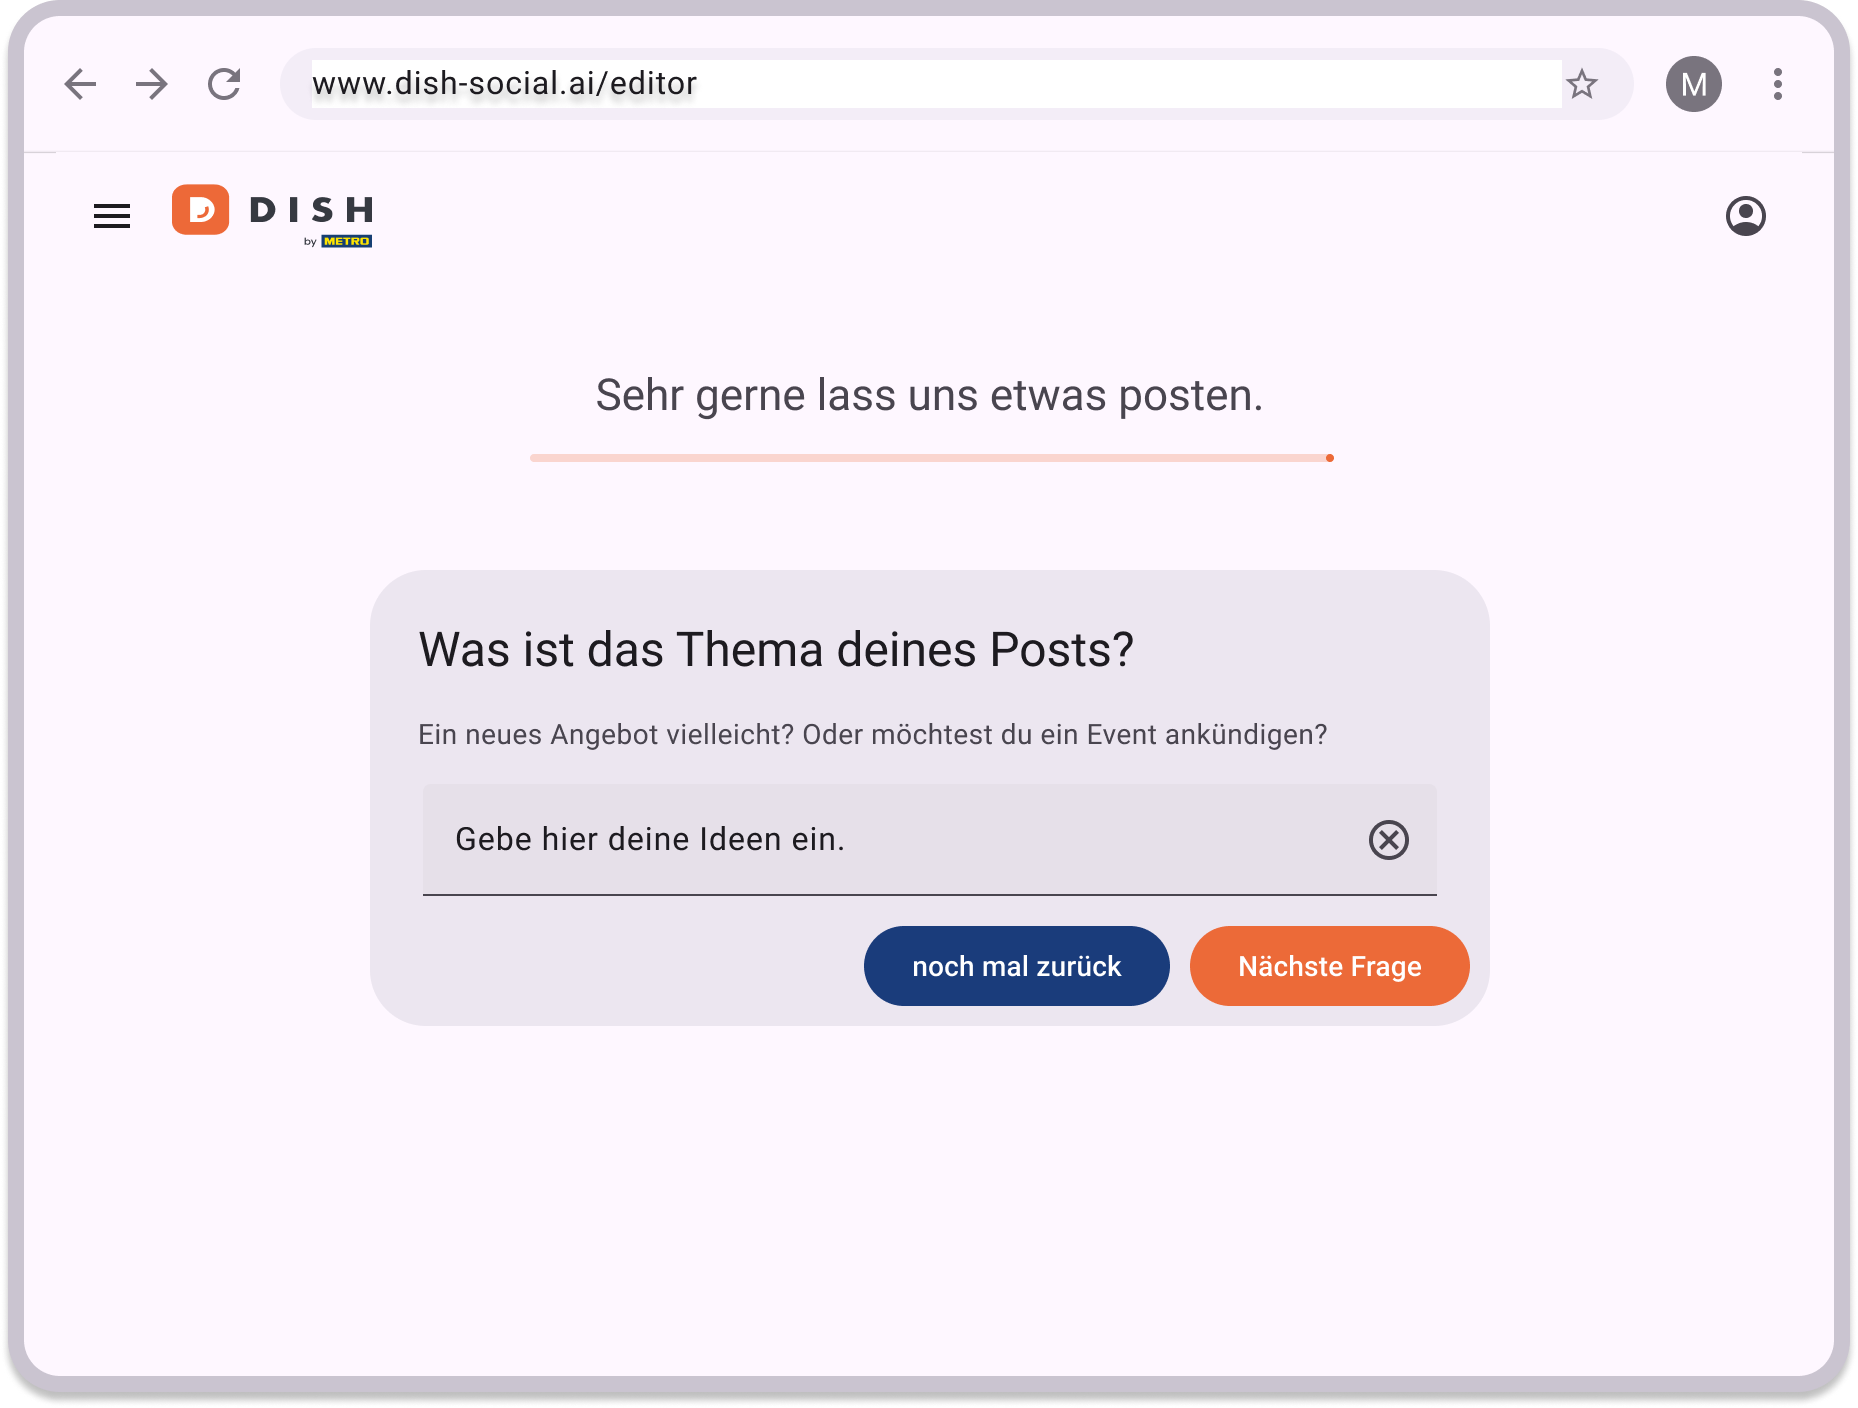
\includegraphics[width=\textwidth]{abbildungen/figma/Editor}
    \caption[]{Figma Design Editor Darstellung}
    \label{fig:editor-page}
    \raggedright Quelle: Eigene Darstellung
\end{figure}
\newpage

\begin{figure}[htbp]
    \centering
    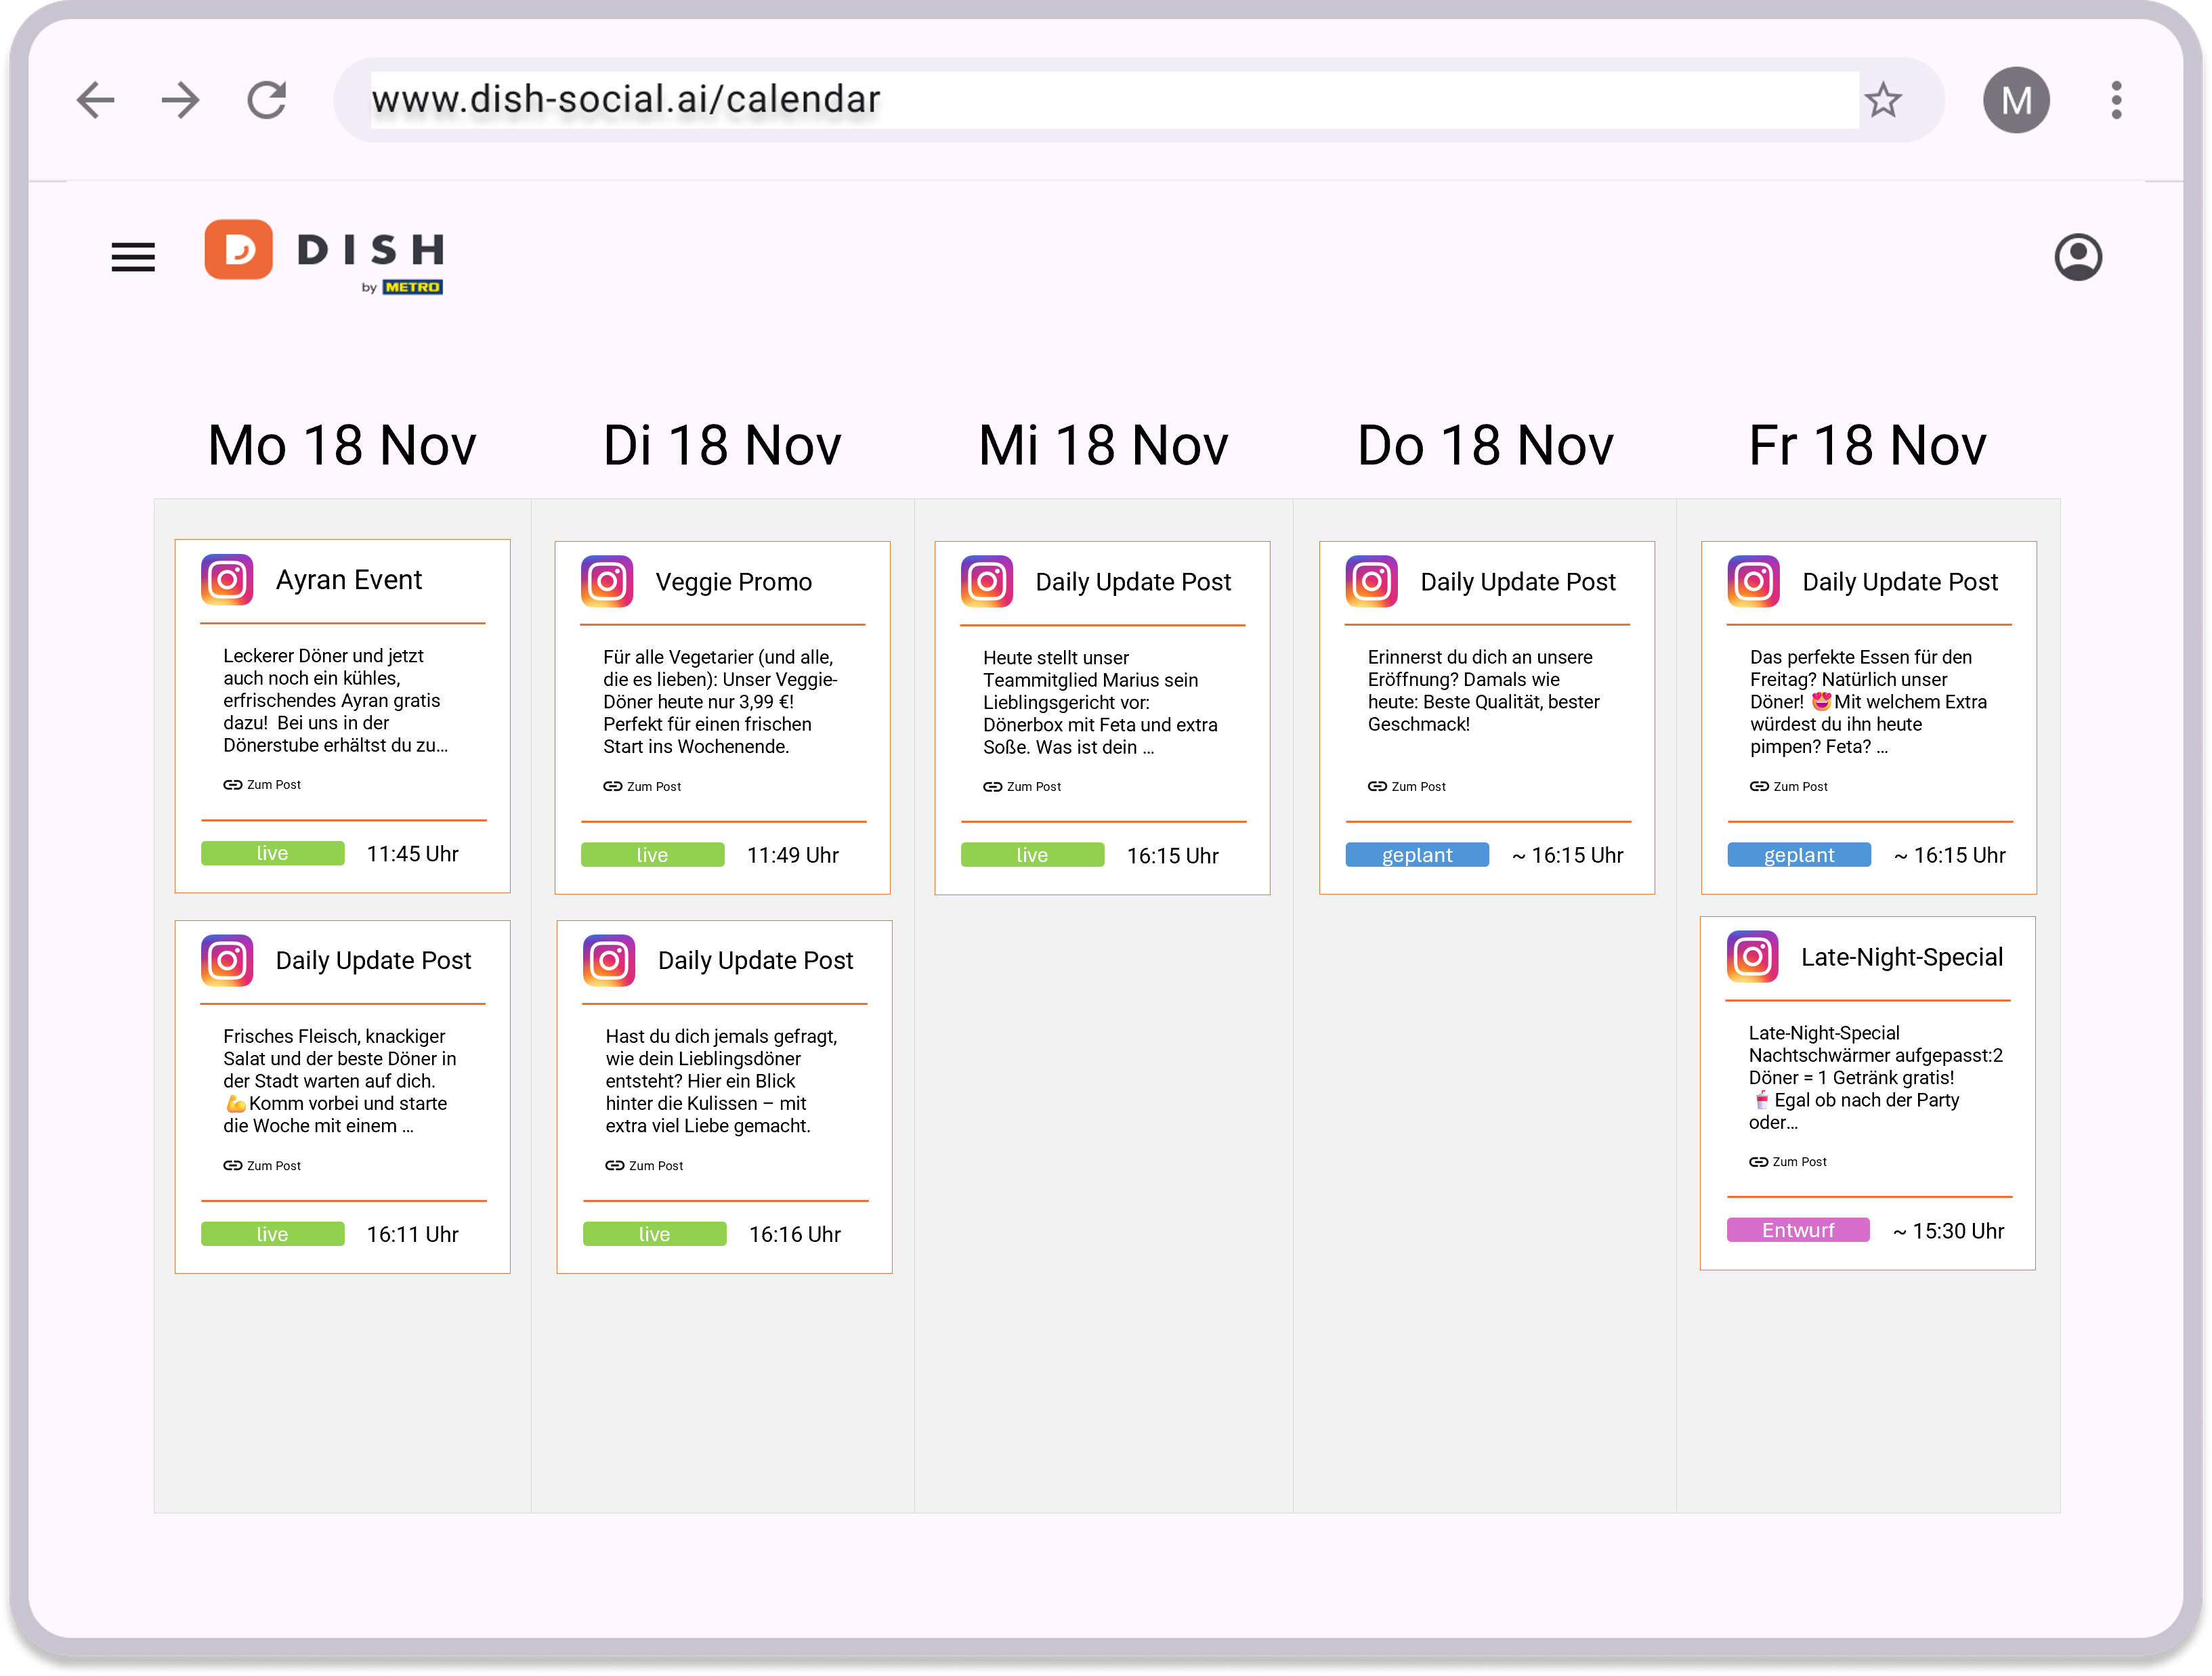
\includegraphics[width=\textwidth]{abbildungen/figma/Kalender}
    \caption[]{Figma Design Kalender Darstellung}
    \label{fig:calendar-page}
    \raggedright Quelle: Eigene Darstellung
\end{figure}

\section{Ergebnisse der Textgenerierung}\label{sec:bilder-textergebnisse}

\begin{figure}[htbp]
    \centering
    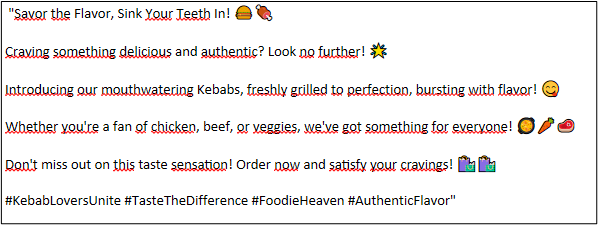
\includegraphics[width=\textwidth]{abbildungen/textresult_mistral}
    \caption[]{generierter Text durch das Text-to-Text Modell mistralai/Mistral-7B-Instruct-v0.3}
    \label{fig:textresult_mistral}
    \raggedright Quelle: Eigene Darstellung
\end{figure}

\begin{figure}[htbp]
    \centering
    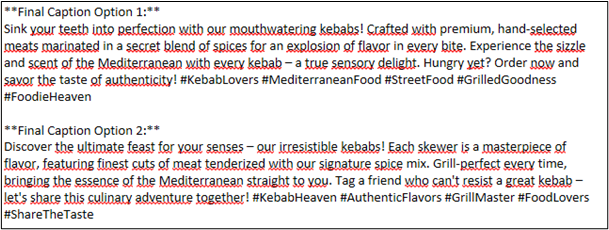
\includegraphics[width=\textwidth]{abbildungen/textresult_Qwen}
    \caption[]{generierter Text durch das Text-to-Text Modell Qwen/QwQ-32B-Preview}
    \label{fig:textresult_Qwen}
    \raggedright Quelle: Eigene Darstellung
\end{figure}

\begin{figure}[htbp]
    \centering
    
\includegraphics[width=\textwidth]{abbildungen/textresult_nvdia_nemotron}
    \caption[]{generierter Text durch das Text-to-Text Modell nvidia/Llama-3.1-Nemotron-70B-Instruct-HF}
    \label{fig:textresult_nvdia_nemotron}
    \raggedright Quelle: Eigene Darstellung
\end{figure}

\end{appendices}
\addtocontents{toc}{\protect\setcounter{tocdepth}{2}}

%-----------------------------------
% Literaturverzeichnis
%-----------------------------------
\newpage

% Die folgende Zeile trägt ALLE Werke aus literatur.bib in das
% Literaturverzeichnis ein, egal ob sie zietiert wurden oder nicht.
% Der Befehl ist also nur zum Test der Skripte sinnvoll und muss bei echten
% Arbeiten entfernt werden.
%\nocite{*}

%\addcontentsline{toc}{section}{Literatur}

% Die folgenden beiden Befehle würden ab dem Literaturverzeichnis wieder eine
% römische Seitennummerierung nutzen.
% Das ist nach dem Leitfaden nicht zu tun. Dort steht nur dass 'sämtliche
% Verzeichnisse VOR dem Textteil' römisch zu nummerieren sind. (vgl. S. 3)
%\pagenumbering{Roman} %Zähler wieder römisch ausgeben
%\setcounter{page}{4}  %Zähler manuell hochsetzen

% Ausgabe des Literaturverzeichnisses

% Keine Trennung der Werke im Literaturverzeichnis nach ihrer Art
% (Online/nicht-Online)
%\begin{RaggedRight}
%\printbibliography
%\end{RaggedRight}

% Alternative Darstellung, die laut Leitfaden genutzt werden sollte.
% Dazu die Zeilen auskommentieren und folgenden code verwenden:

% Literaturverzeichnis getrennt nach Nicht-Online-Werken und Online-Werken
% (Internetquellen).
% Die Option nottype=online nimmt alles, was kein Online-Werk ist.
% Die Option heading=bibintoc sorgt dafür, dass das Literaturverzeichnis im
% Inhaltsverzeichnis steht.
% Es ist übrigens auch möglich mehrere type- bzw. nottype-Optionen anzugeben, um
% noch weitere Arten von Zusammenfassungen eines Literaturverzeichnisse zu
% erzeugen.
% Beispiel: [type=book,type=article]
\printbibliography[nottype=online,heading=bibintoc,title={\langde{Literaturverzeichnis}\langen{Bibliography}}]

% neue Seite für Internetquellen-Verzeichnis
\newpage

% Laut Leitfaden 2018, S. 14, Fussnote 44 stehen die Internetquellen NICHT im
% Inhaltsverzeichnis, sondern gehören zum Literaturverzeichnis.
% Die Option heading=bibintoc würde die Internetquelle als eigenen Eintrag im
% Inhaltsverzeicnis anzeigen.
%\printbibliography[type=online,heading=bibintoc,title={\headingNameInternetSources}]
\printbibliography[type=online,heading=subbibliography,title={\headingNameInternetSources}]

\newpage
\pagenumbering{gobble} % Keine Seitenzahlen mehr

%-----------------------------------
% Ehrenwörtliche Erklärung
%-----------------------------------
\section*{%
	\langde{Ehrenwörtliche Erklärung}
	\langen{Declaration in lieu of oath}}
\langde{Hiermit versicheren wir, dass die vorliegende Arbeit von uns selbstständig und ohne unerlaubte Hilfe angefertigt worden ist,
	insbesondere dass alle Stellen, die wörtlich oder annähernd wörtlich aus Veröffentlichungen entnommen sind, durch Zitate als solche gekennzeichnet wurden.
	Wir versicheren auch, dass die von uns eingereichte schriftliche Version mit der digitalen Version übereinstimmt.
	Weiterhin erklären wir, dass die Arbeit in gleicher oder ähnlicher Form noch keiner Prüfungsbehörde/Prüfungsstelle vorgelegen hat.
	Wir erklären uns damit \textcolor{red}{einverstanden}, dass die Arbeit der Öffentlichkeit zugänglich gemacht wird.
	Wir erklären uns damit einverstanden, dass die Digitalversion dieser Arbeit zwecks Plagiatsprüfung auf die Server externer Anbieter hochgeladen werden darf.
	Die Plagiatsprüfung stellt keine Zurverfügungstellung für die Öffentlichkeit dar.}

\langen{I/We hereby declare that I/we produced the submitted paper with no assistance from any other party and without the use of any unauthorized aids and, in particular, that I/we have marked as quotations all passages which are reproduced verbatim or near-verbatim from publications. Also, I/We declare that the submitted print version of this thesis is identical with its digital version. Further, I/We declare that this thesis has never been submitted before to any examination board in either its present form or in any other similar version. I/We herewith \textcolor{red}{agree/disagree} that this thesis may be published. I/We herewith consent that this thesis may be uploaded to the server of external contractors for the purpose of submitting it to the contractors’ plagiarism detection systems. Uploading this thesis for the purpose of submitting it to plagiarism detection systems is not a form of publication.}


\par\medskip
\par\medskip

\vspace{4cm}

\begin{table}[H]
	\centering
	\begin{tabular*}{\textwidth}{@{\extracolsep{\fill}} c l c}
		\langde{Alexander Langel} & \langde{Duisburg, \the\day.\the\month.\the\year} & \rule[0.5ex]{15em}{0.55pt} \\
		\vspace{2cm} \\

		\langde{Mike Miemczok} & \langde{Mülheim, \the\day.\the\month.\the\year} & \rule[0.5ex]{15em}{0.55pt} \\
		\vspace{2cm} \\

		\langde{Marius Jahnke} & \langde{Bochum, \the\day.\the\month.\the\year} & \rule[0.5ex]{15em}{0.55pt} \\
	\end{tabular*}
\end{table}


\end{document}
